\section{Results}
\label{sec:results}

We have implemented and tested our methods on 26 different real-world datasets.
The vast majority of datasets studied were sourced from Outlier Detection Datasets (ODDS), which provided clear labels for normal and anomalous behavior.
We examine the effectiveness of our methods by their ability to identify these outliers.

Figure~\ref{results:datasets} shows % TODO
We chose to use so many different real world datasets to ensure that our methods could generalize to many target audiences.

\begin{figure*}[!t]
\centering
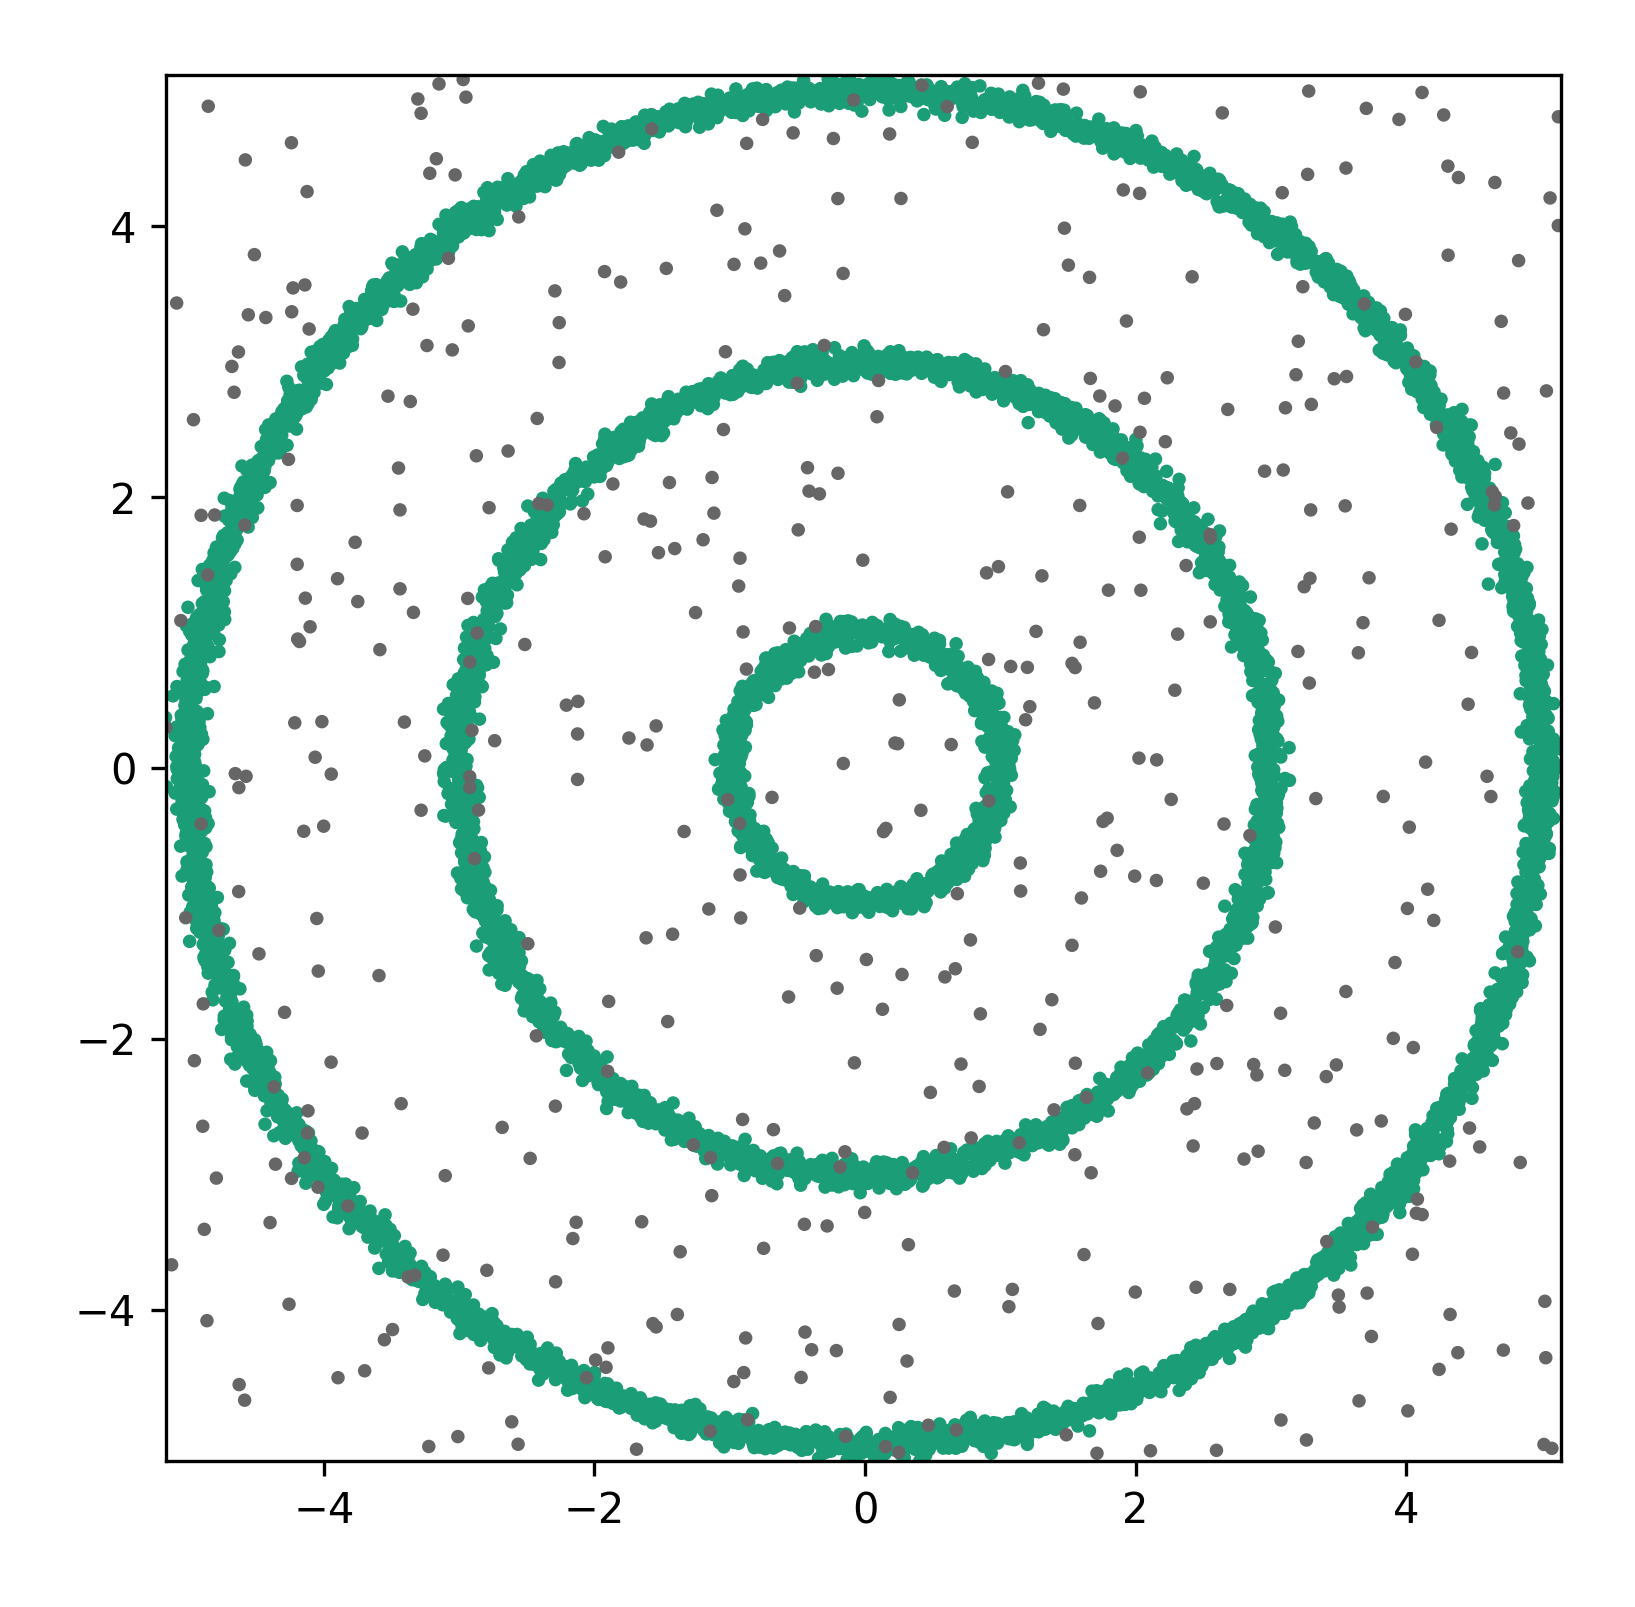
\includegraphics[width=2.5in]{static/bullseye.png}
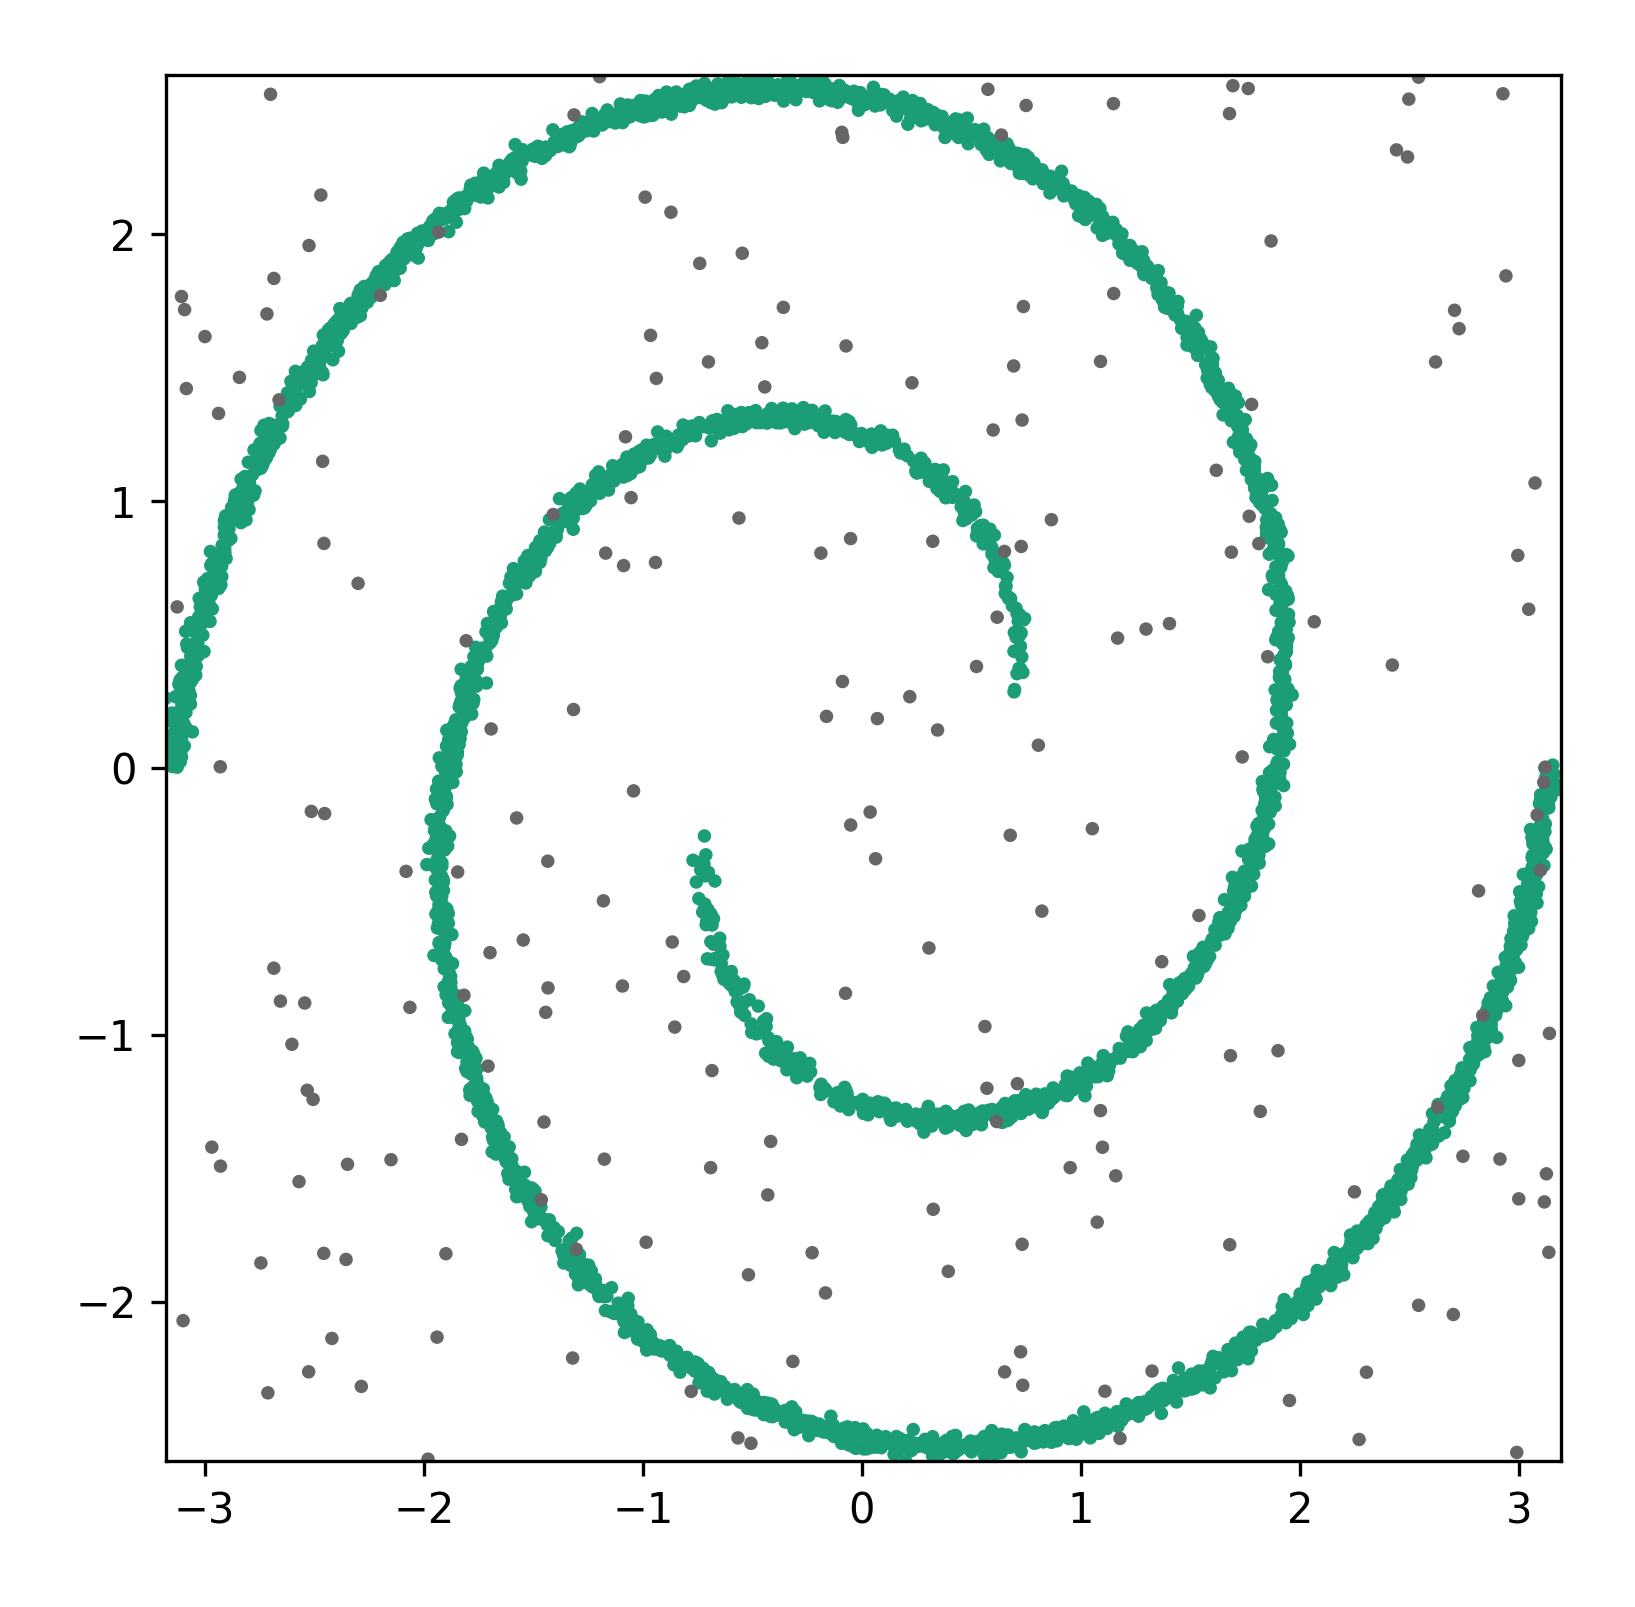
\includegraphics[width=2.5in]{static/spiral.png}
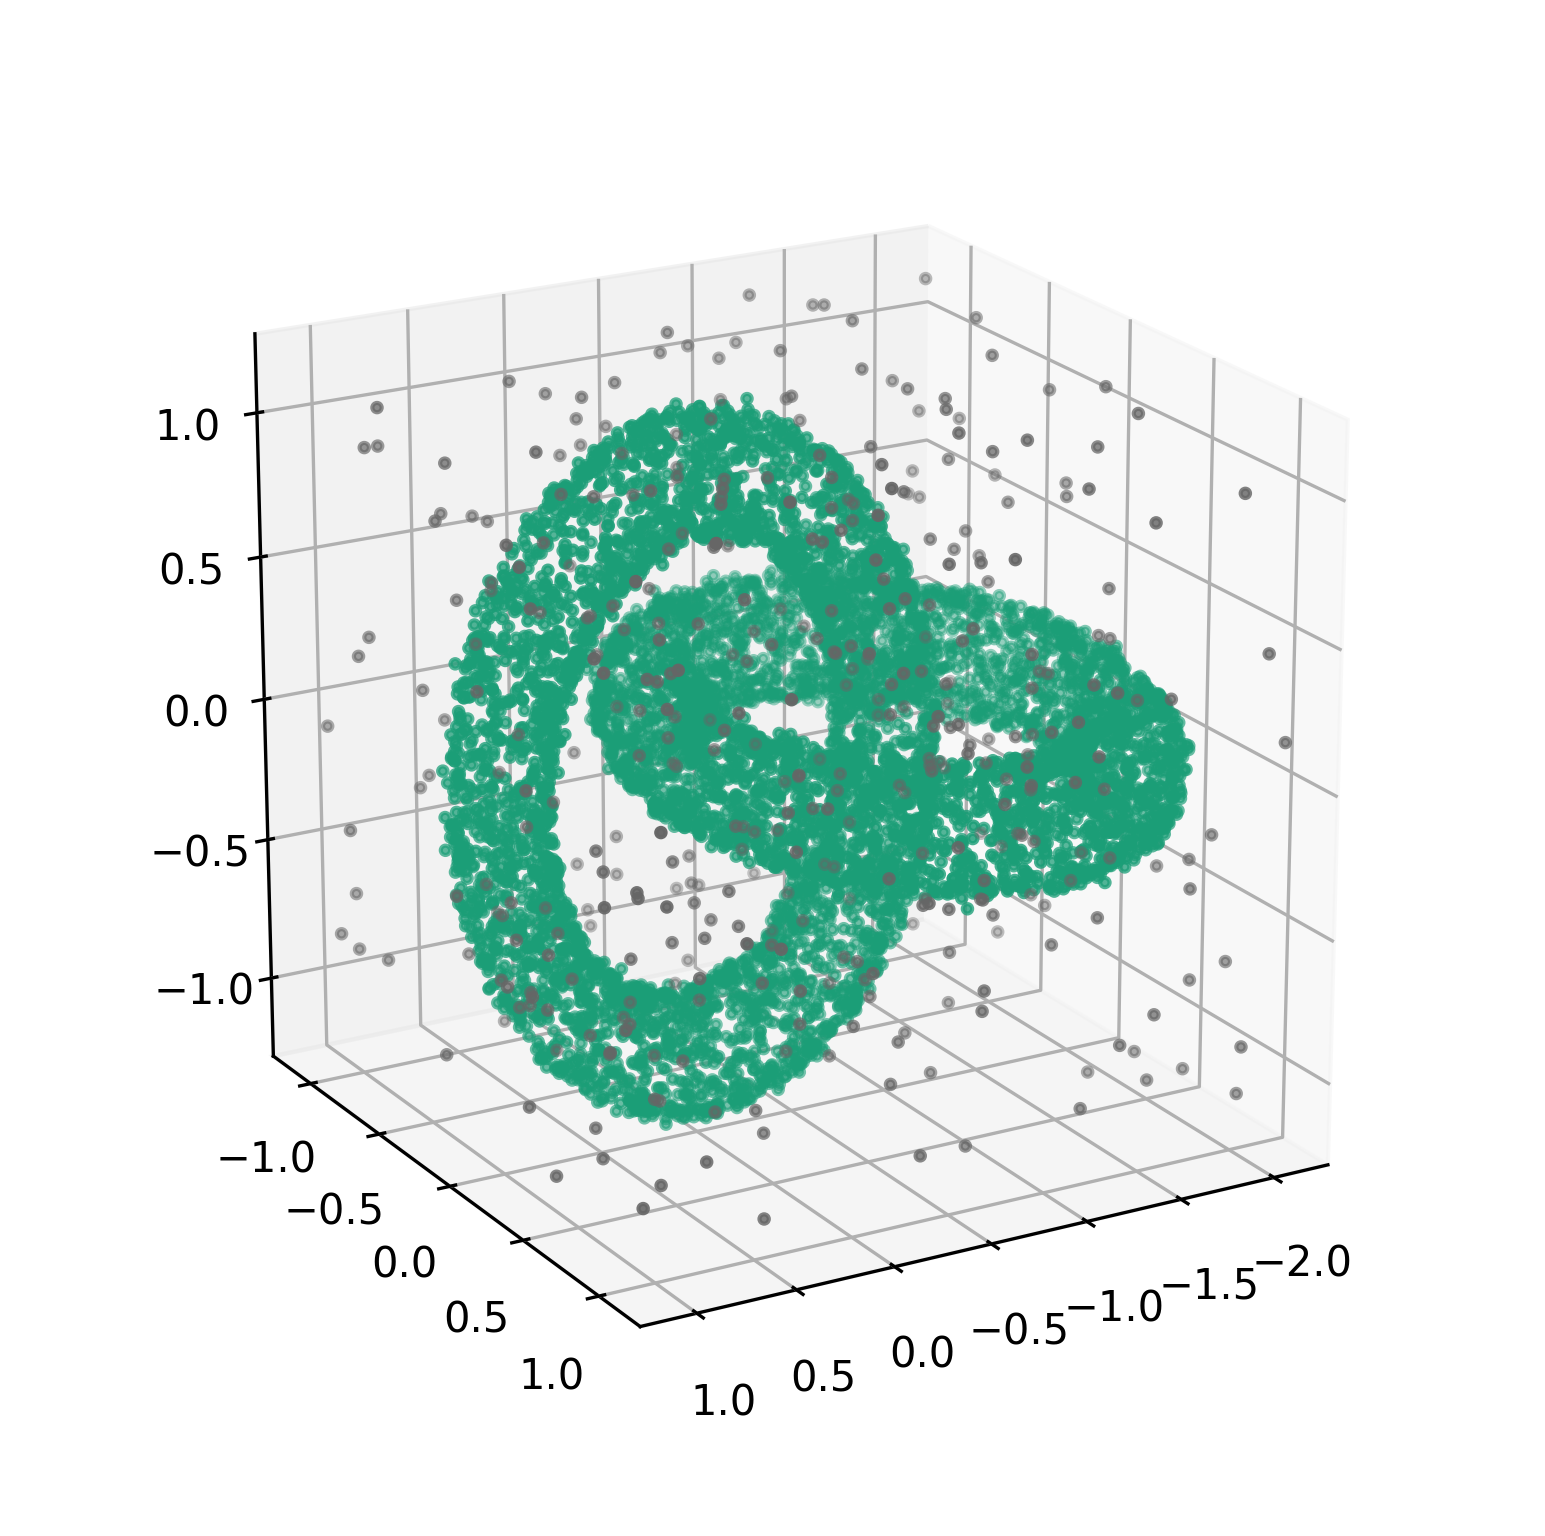
\includegraphics[width=3in]{static/interlocking_tori.png}
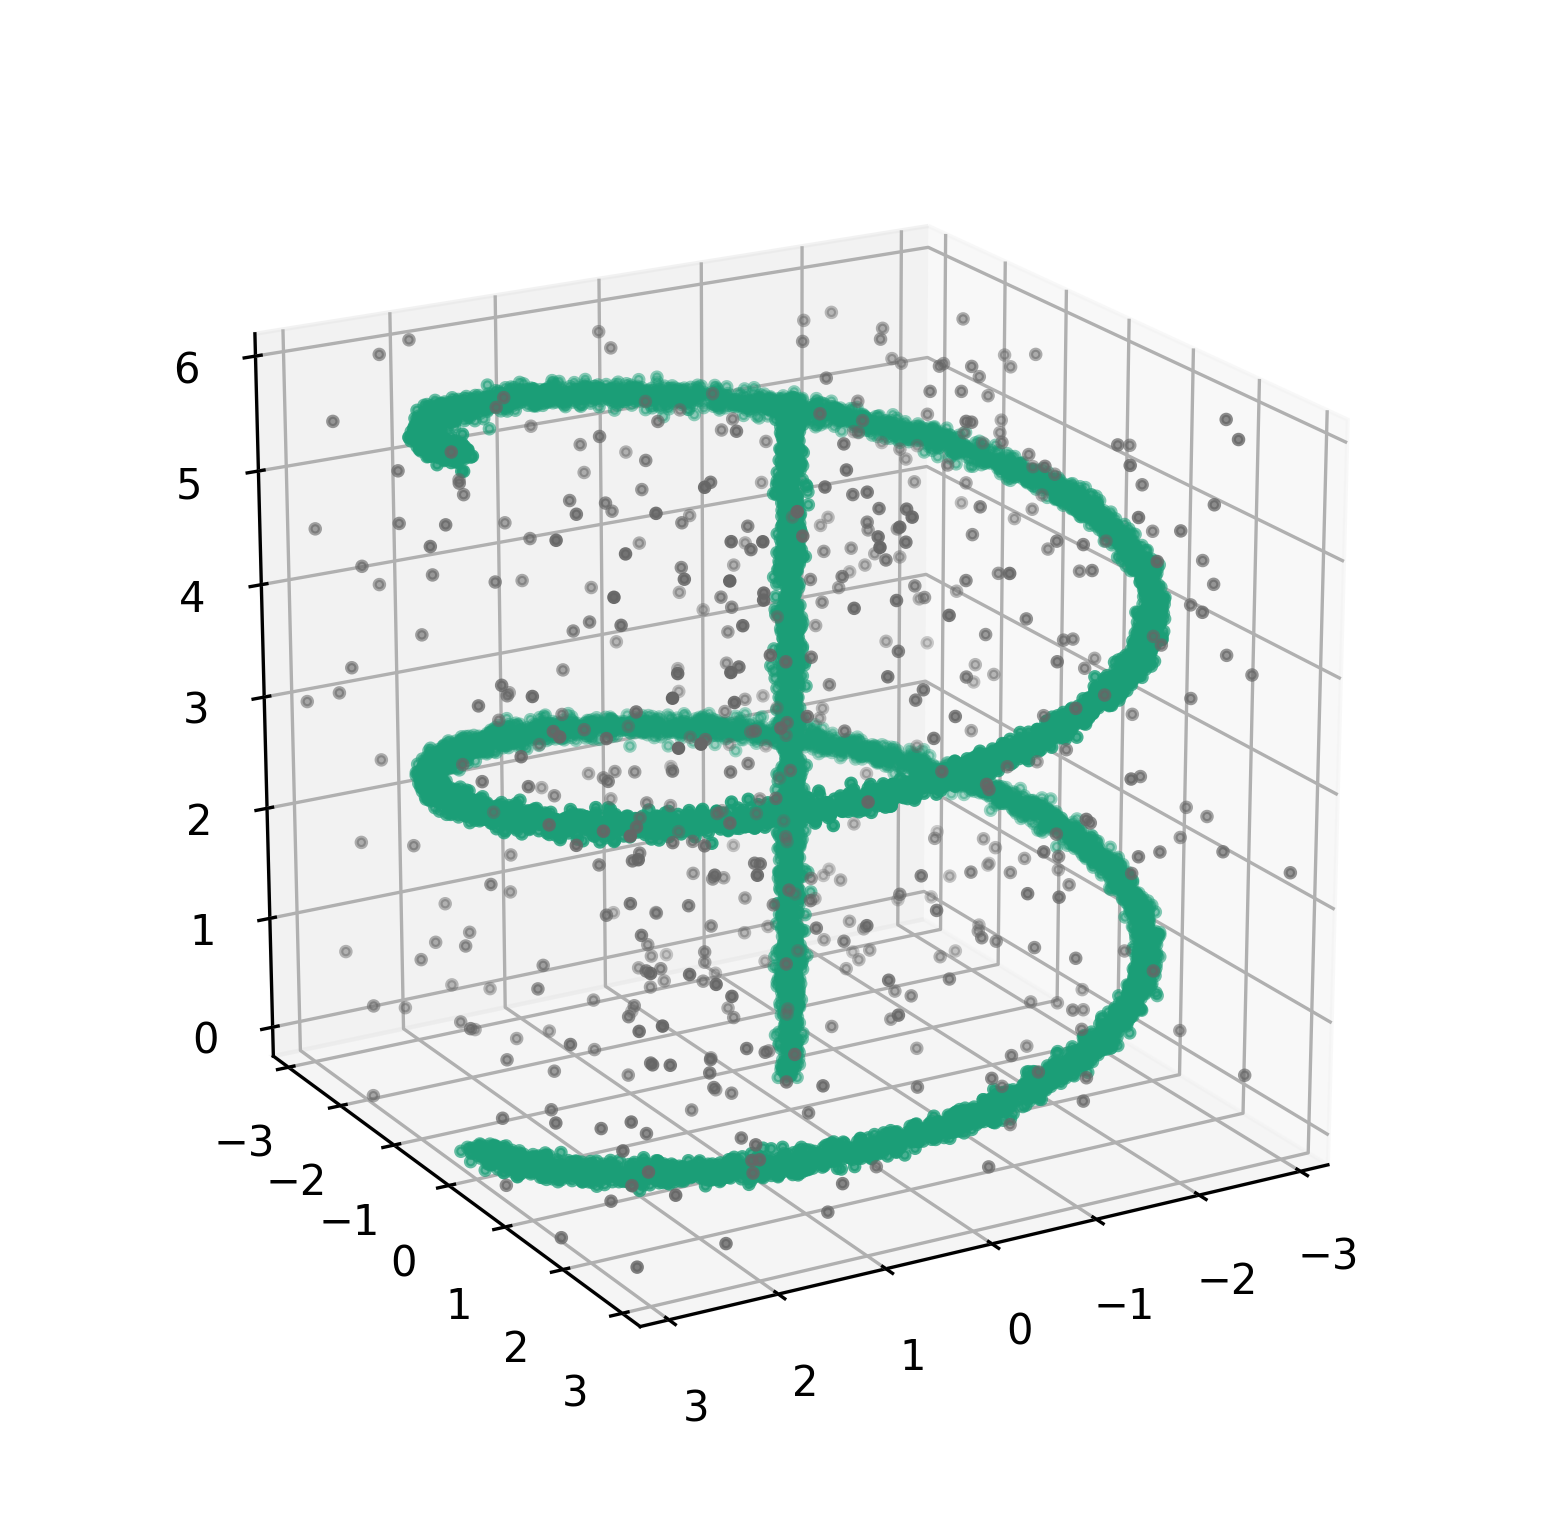
\includegraphics[width=3in]{static/skewer.png}
\caption{The Bullseye (top-left), Spiral (top-right), Interlocking Tori (bottom-left) and Skewer (bottom-left) datasets.}
\label{results:datasets}
\end{figure*}

For each dataset, we clustered using Manhattan, Euclidean, and Cosine distance functions.
Additionally, for this work, we allowed CLAM to cluster down until the manifold had thoroughly shattered.
We then iterated over all depths to compute the area under the ROC-Curve.

After computing anomalousness scores, we normalized each metric to a $[0, 1]$ range.
For each dataset, we present a confusion matrix, a ROC curve, and the area under the ROC curve for a sample of optimal depths. 
To demonstrate our methods are not overly-sensitive to depth we present all metrics in a 5-depth wide window.

Table~\ref{results:table} lists % TODO

\begin{table*}[!t]
\renewcommand{\arraystretch}{1.3}
\caption{Comparison of CHAODA with state-of-the-art algorithms}
\label{results:table}
\centering
\begin{tabular}{|c|c|c|c|c|c|c|c|c|c|c|c|c|c|c|c|}
\hline
{\textbf{Dataset}} & {\textbf{Metric}} & {\textbf{Method}} & \multicolumn{3}{c|}{\textbf{AUC ROC}} & \multicolumn{10}{c|}{\textbf{ }} \\
\hline
 &  &  & d - 2 & d & d + 2 &  &  &  &  &  &  &  &  &  & \\
\hline
\bfseries lympho & \bfseries cosine & \bfseries cluster\_cardinality & 0.926 & 0.949 & 0.838 &  &  &  &  &  &  &  &  &  & \\ 
\hline
\bfseries lympho & \bfseries cosine & \bfseries hierarchical & 0.927 & 0.940 & 0.938 &  &  &  &  &  &  &  &  &  & \\ 
\hline
\bfseries lympho & \bfseries cosine & \bfseries k\_neighborhood & 0.500 & 0.888 & 0.725 &  &  &  &  &  &  &  &  &  & \\ 
\hline
\bfseries lympho & \bfseries cosine & \bfseries random\_walk & 0.803 & 0.964 & 0.952 &  &  &  &  &  &  &  &  &  & \\ 
\hline
\bfseries lympho & \bfseries cosine & \bfseries subgraph\_cardinality & 0.583 & 0.739 & 0.729 &  &  &  &  &  &  &  &  &  & \\ 
\hline
\bfseries lympho & \bfseries euclidean & \bfseries cluster\_cardinality & 0.672 & 0.904 & 0.887 &  &  &  &  &  &  &  &  &  & \\ 
\hline
\bfseries lympho & \bfseries euclidean & \bfseries hierarchical & 0.672 & 0.869 & 0.863 &  &  &  &  &  &  &  &  &  & \\ 
\hline
\bfseries lympho & \bfseries euclidean & \bfseries k\_neighborhood & 0.500 & 0.573 & 0.500 &  &  &  &  &  &  &  &  &  & \\ 
\hline
\bfseries lympho & \bfseries euclidean & \bfseries random\_walk & 0.704 & 0.783 & 0.692 &  &  &  &  &  &  &  &  &  & \\ 
\hline
\bfseries lympho & \bfseries euclidean & \bfseries subgraph\_cardinality & 0.500 & 0.500 & 0.500 &  &  &  &  &  &  &  &  &  & \\ 
\hline
\bfseries lympho & \bfseries manhattan & \bfseries cluster\_cardinality & 0.793 & 0.965 & 0.962 &  &  &  &  &  &  &  &  &  & \\ 
\hline
\bfseries lympho & \bfseries manhattan & \bfseries hierarchical & 0.935 & 0.965 & 0.955 &  &  &  &  &  &  &  &  &  & \\ 
\hline
\bfseries lympho & \bfseries manhattan & \bfseries k\_neighborhood & 0.648 & 0.818 & 0.818 &  &  &  &  &  &  &  &  &  & \\ 
\hline
\bfseries lympho & \bfseries manhattan & \bfseries random\_walk & 0.763 & 0.960 & 0.955 &  &  &  &  &  &  &  &  &  & \\ 
\hline
\bfseries lympho & \bfseries manhattan & \bfseries subgraph\_cardinality & 0.583 & 0.663 & 0.660 &  &  &  &  &  &  &  &  &  & \\ 
\hline

\end{tabular}
\end{table*}

\begin{figure*}[!t]
\centering
% Annthyroid
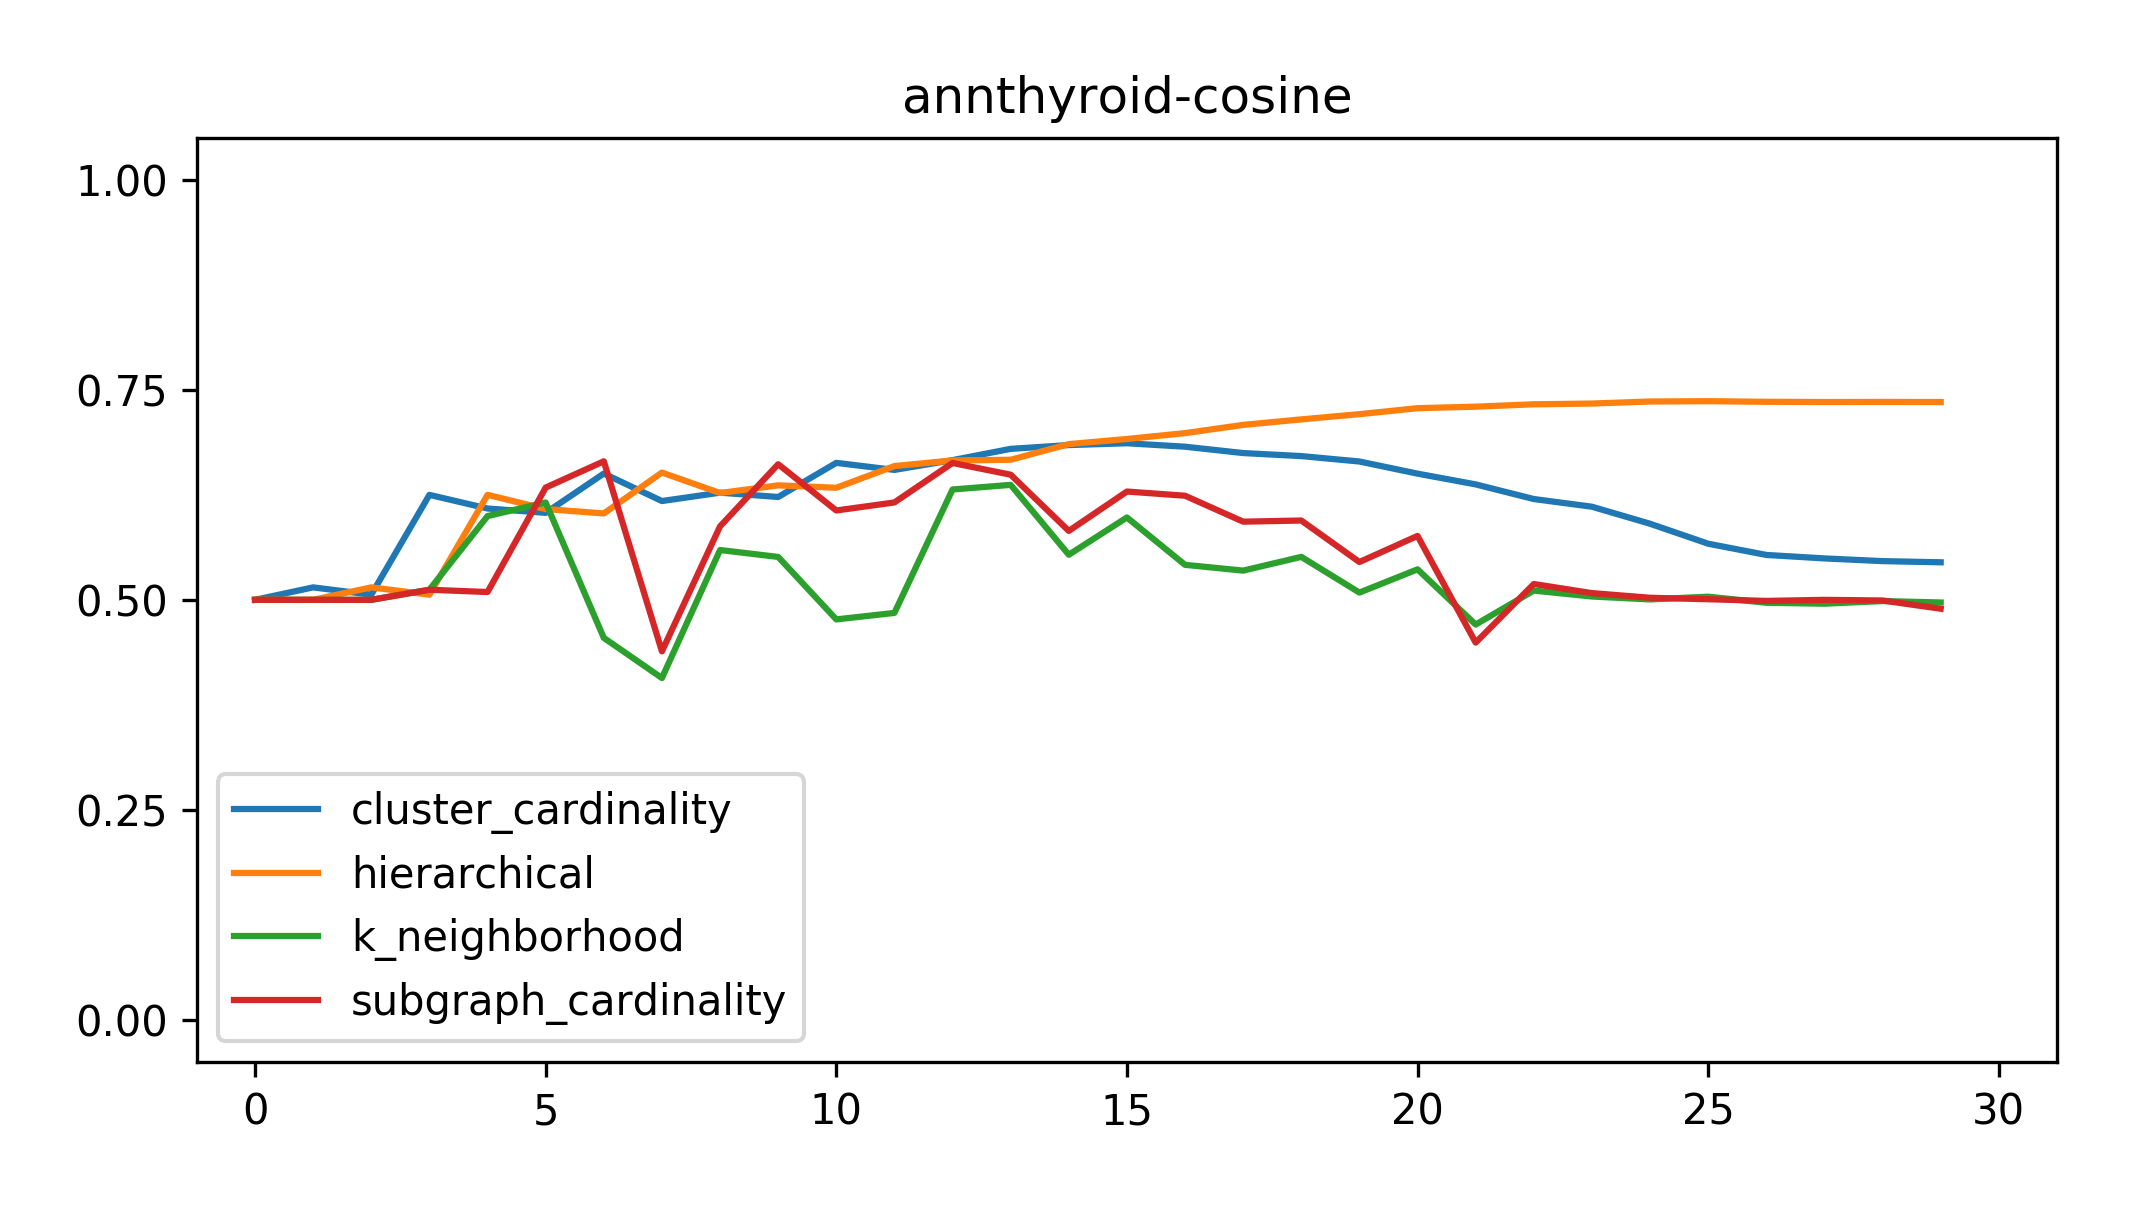
\includegraphics[width=2.2in]{kdd/static/auc_vs_depth/annthyroid-cosine.png}
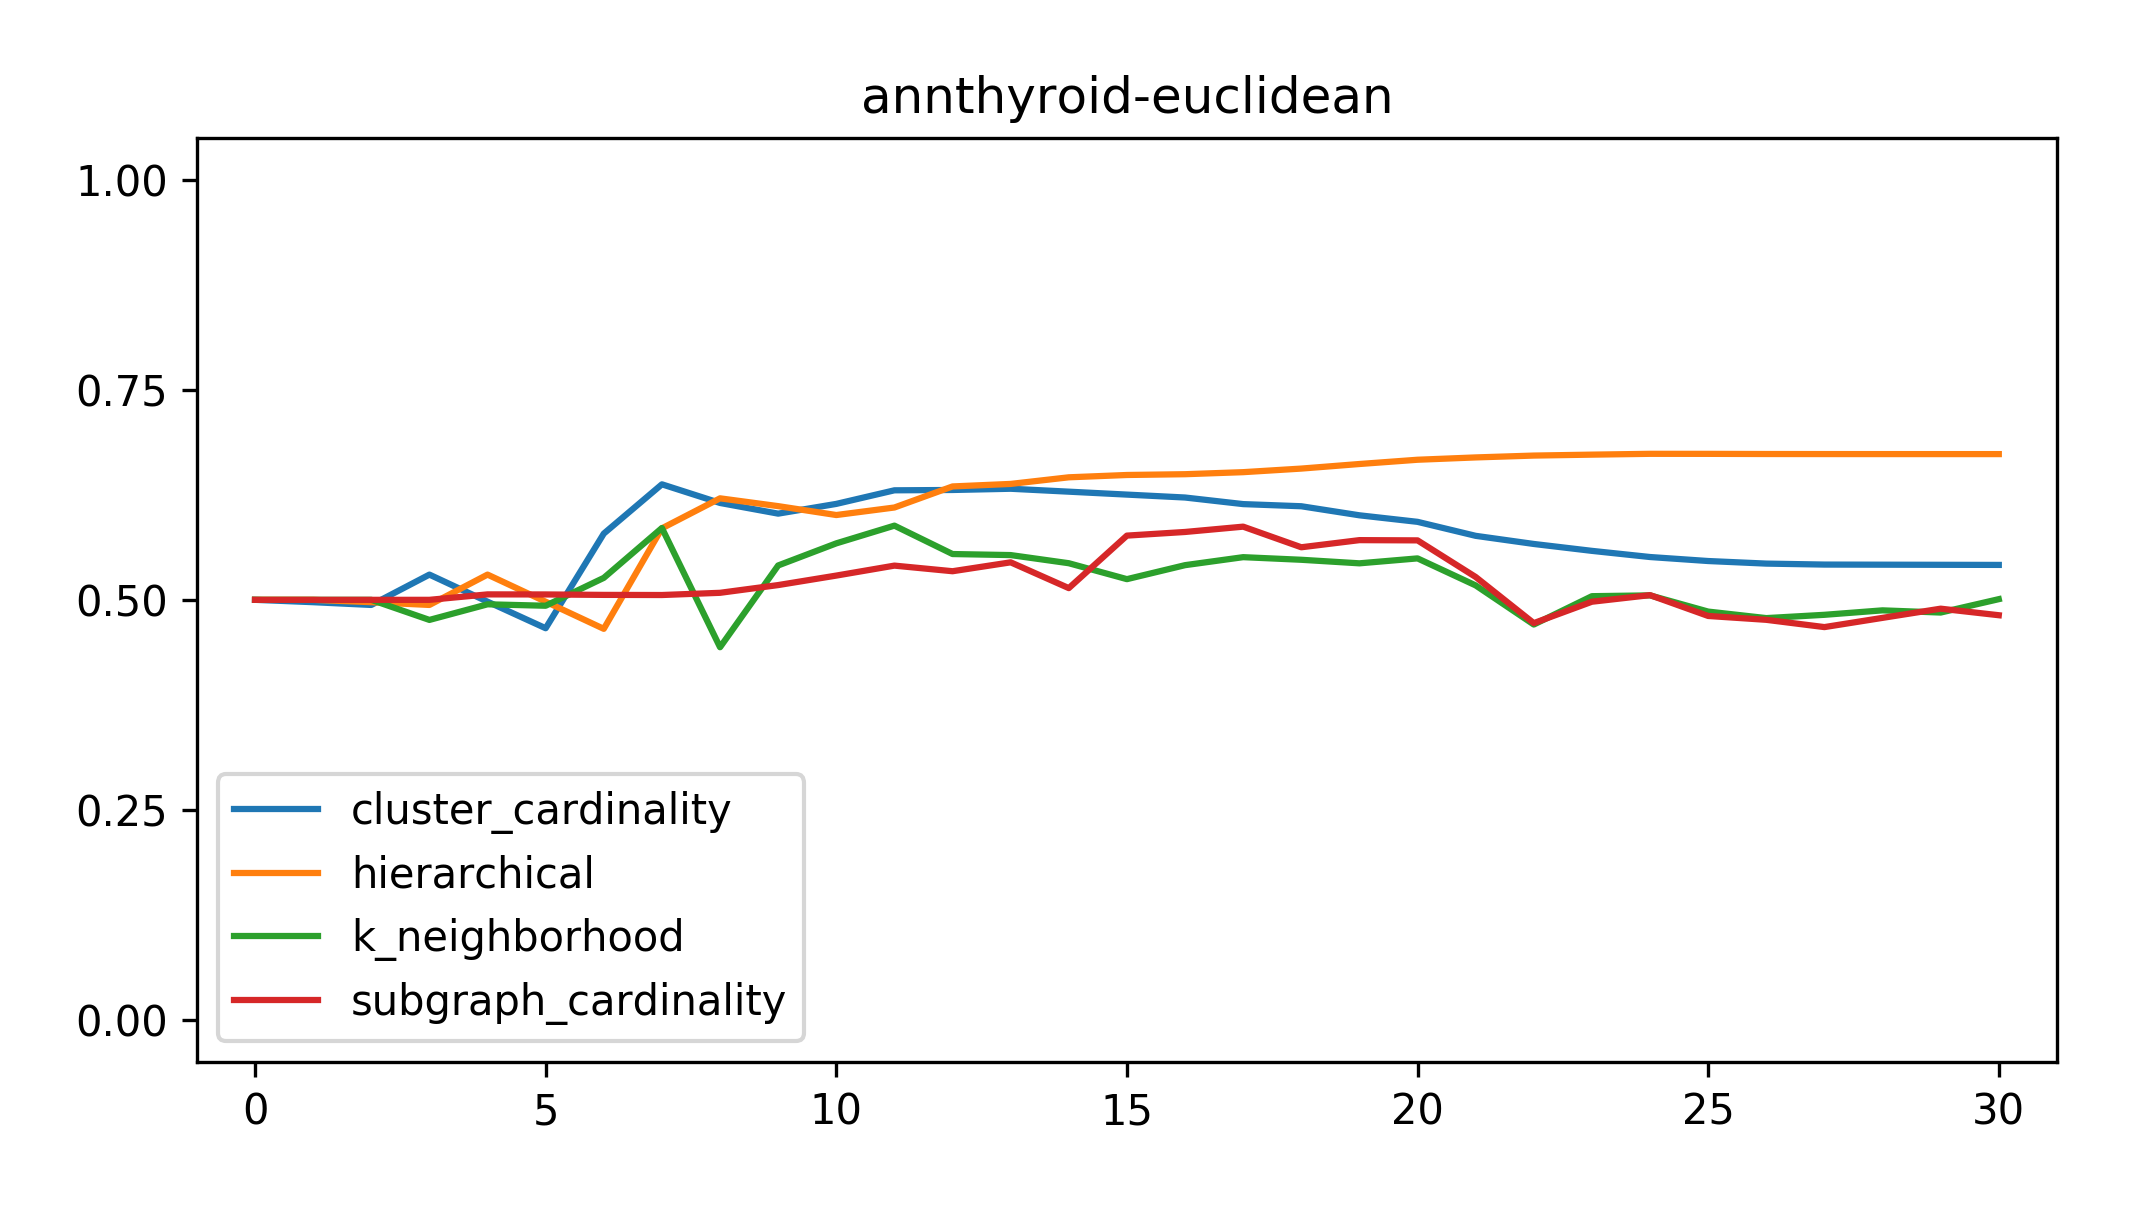
\includegraphics[width=2.2in]{kdd/static/auc_vs_depth/annthyroid-euclidean.png}
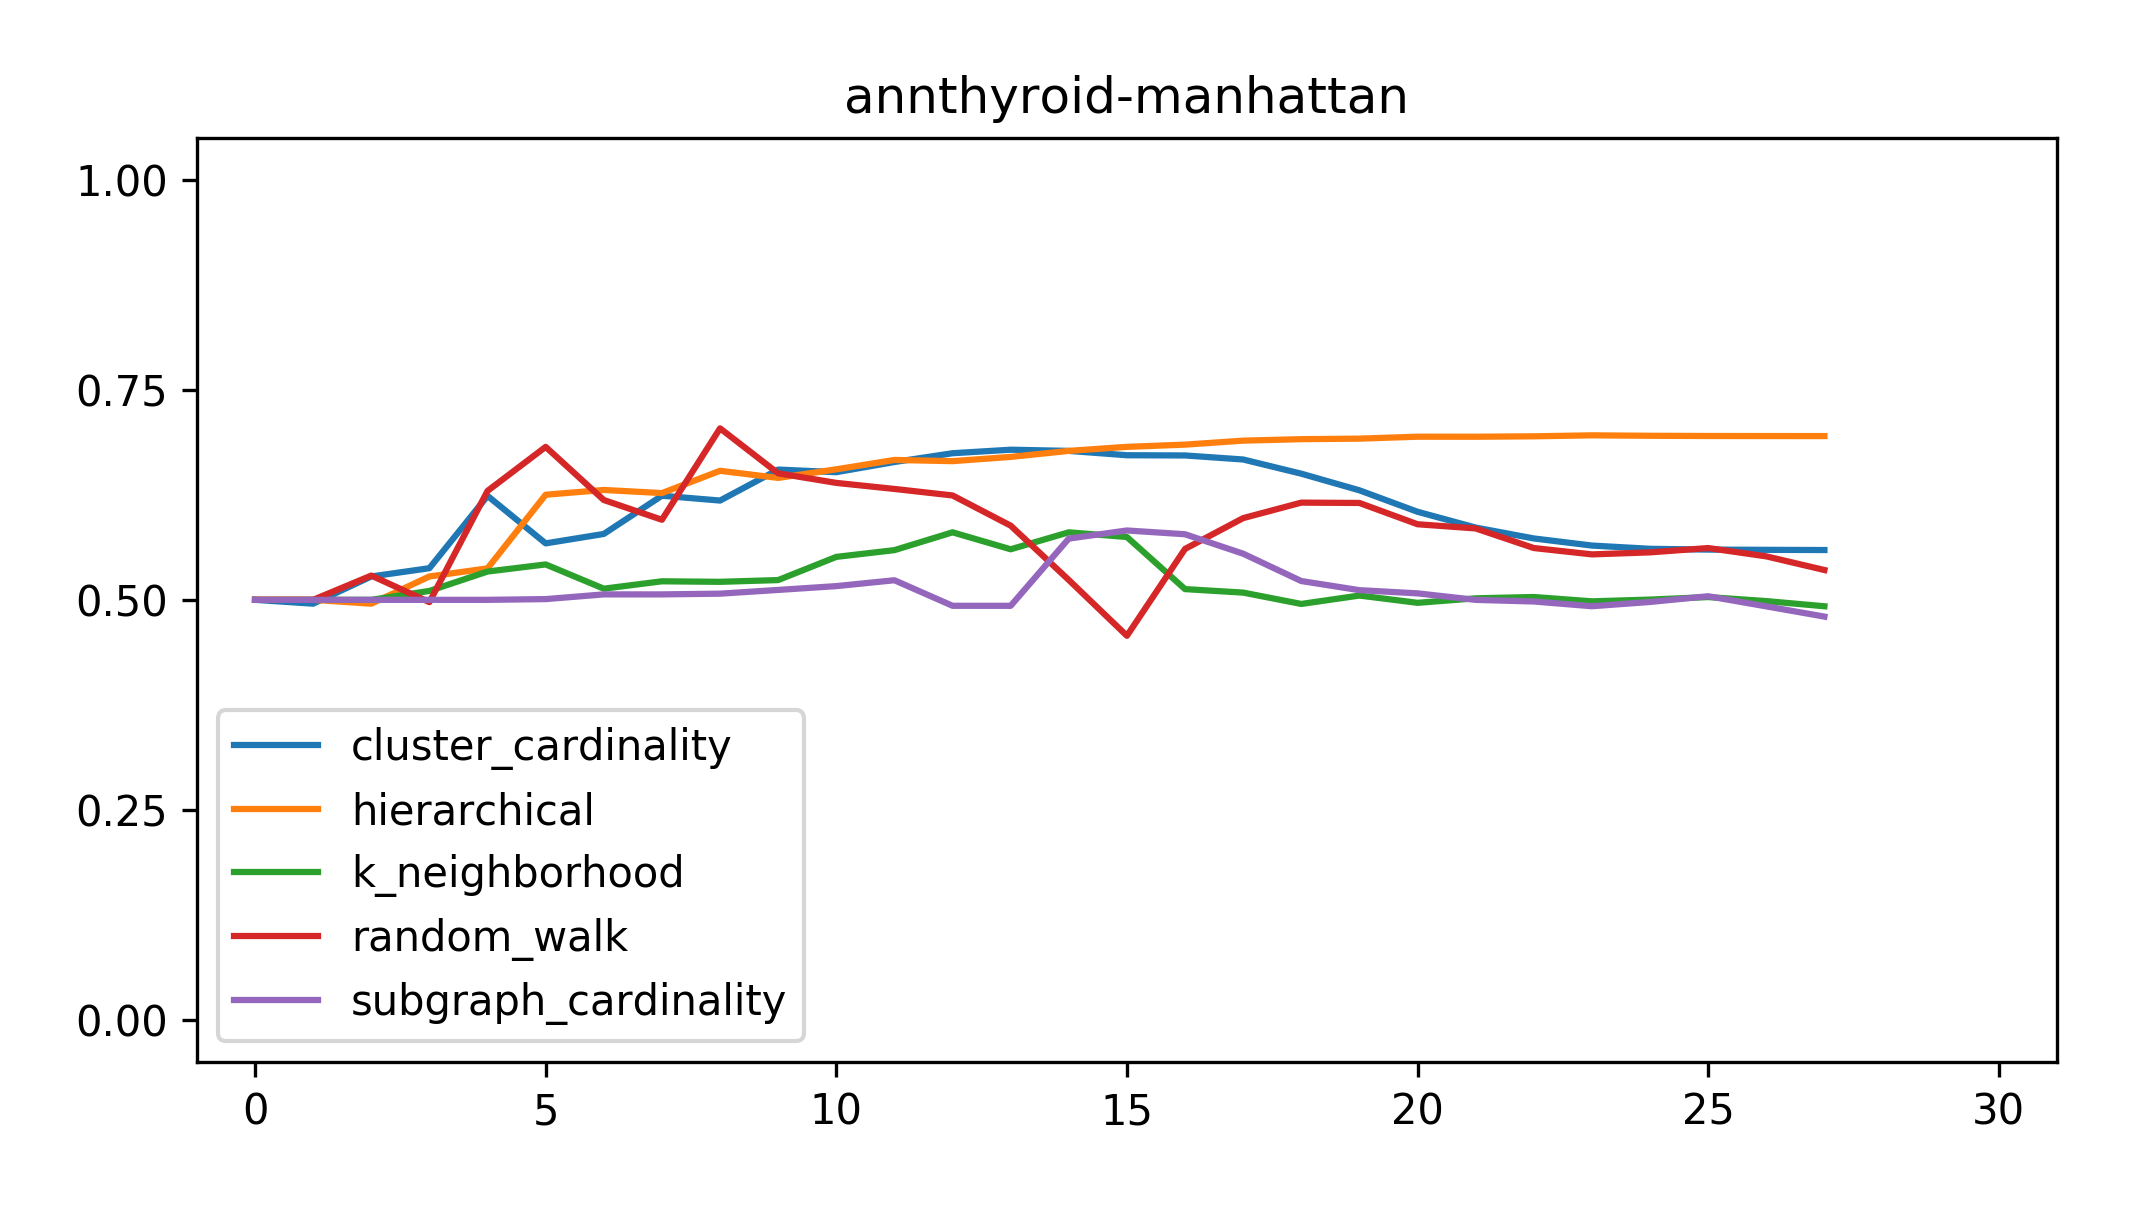
\includegraphics[width=2.2in]{kdd/static/auc_vs_depth/annthyroid-manhattan.png}

% Arrhythmia
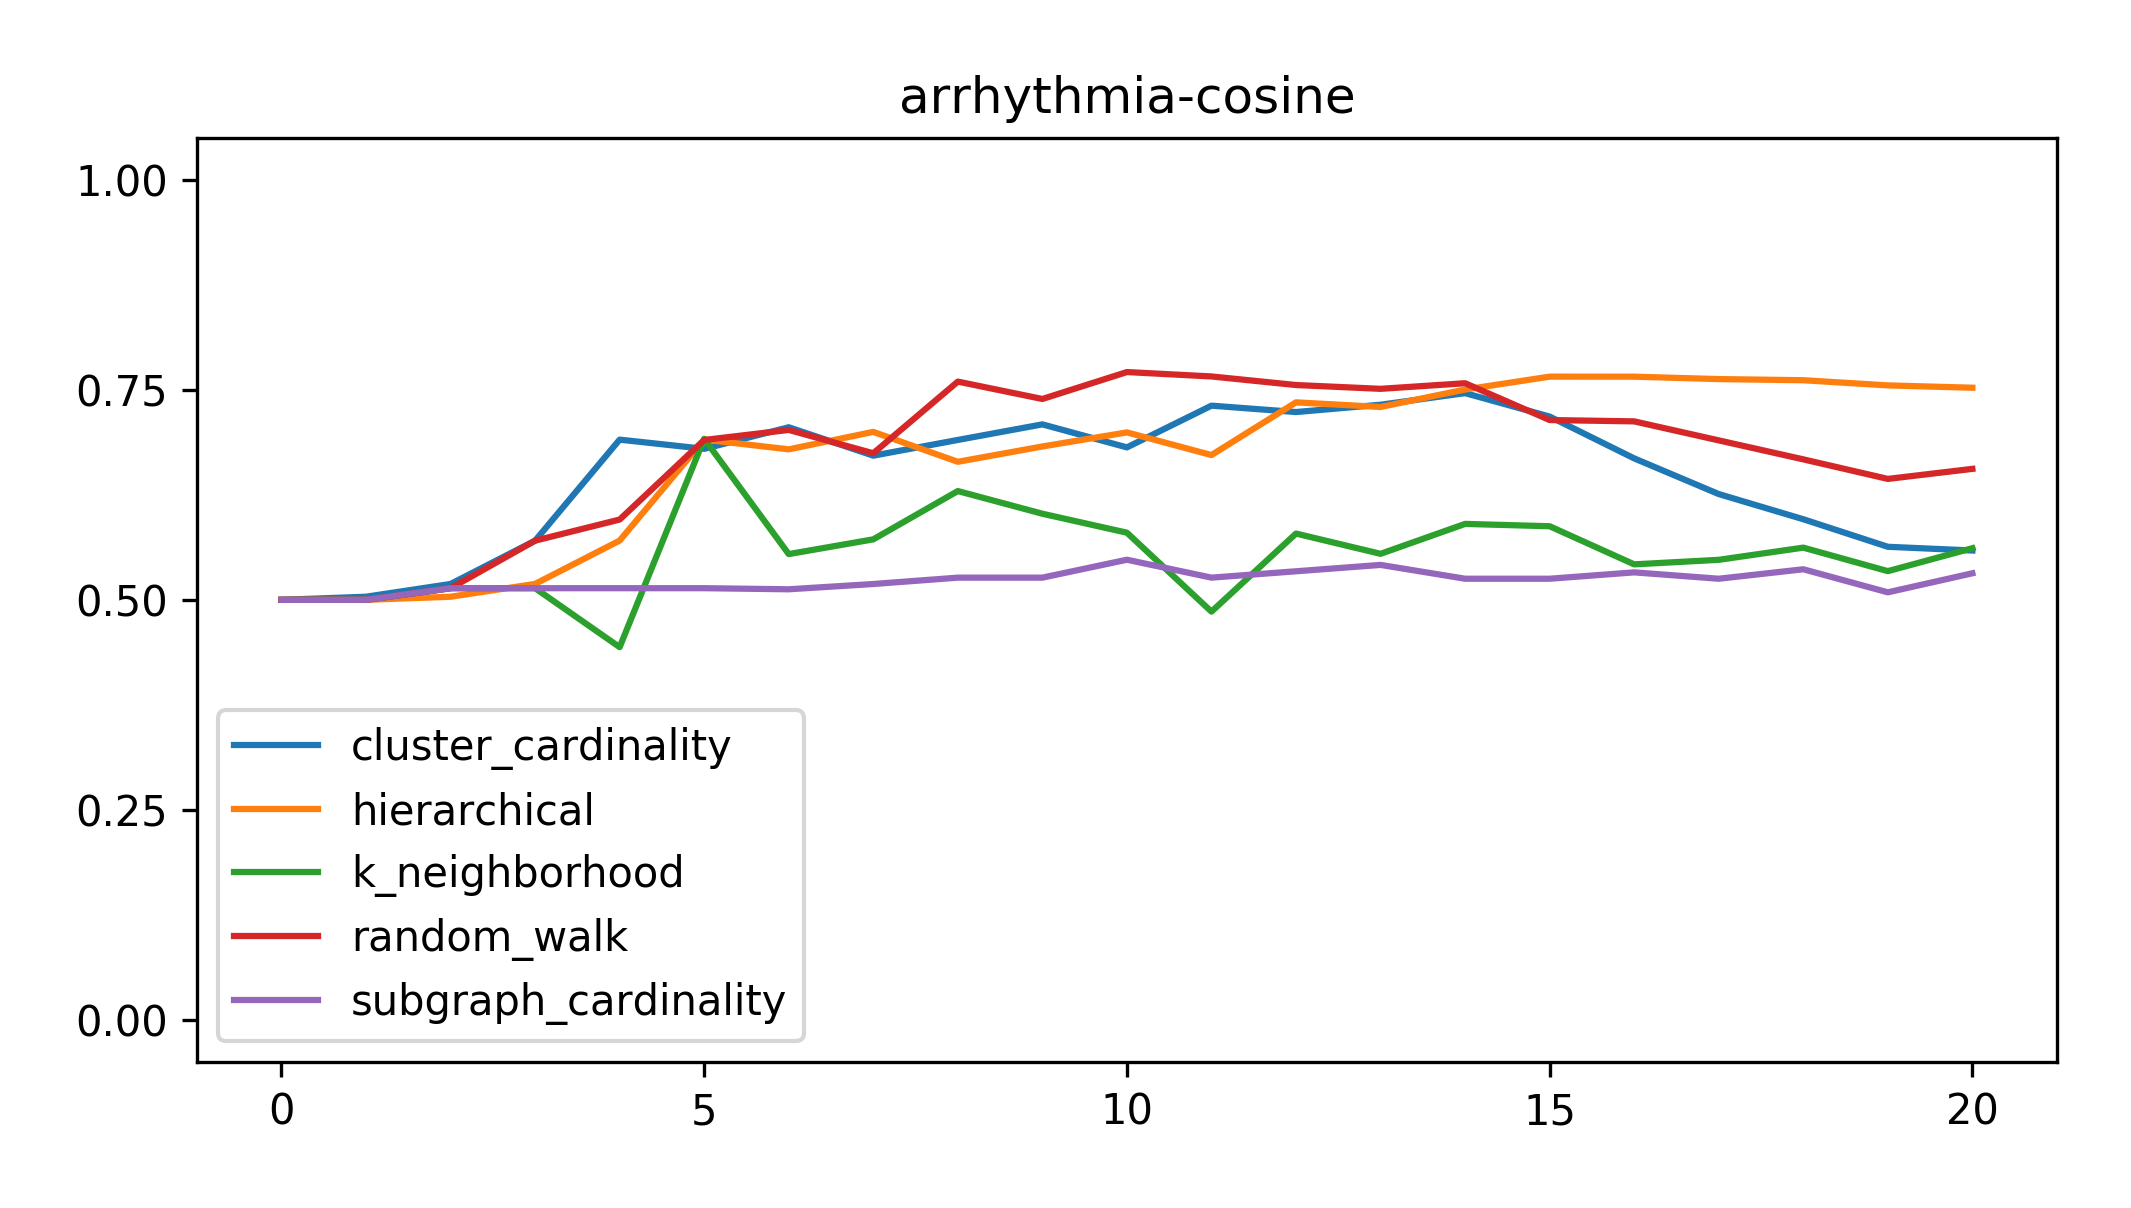
\includegraphics[width=2.2in]{kdd/static/auc_vs_depth/arrhythmia-cosine.png}
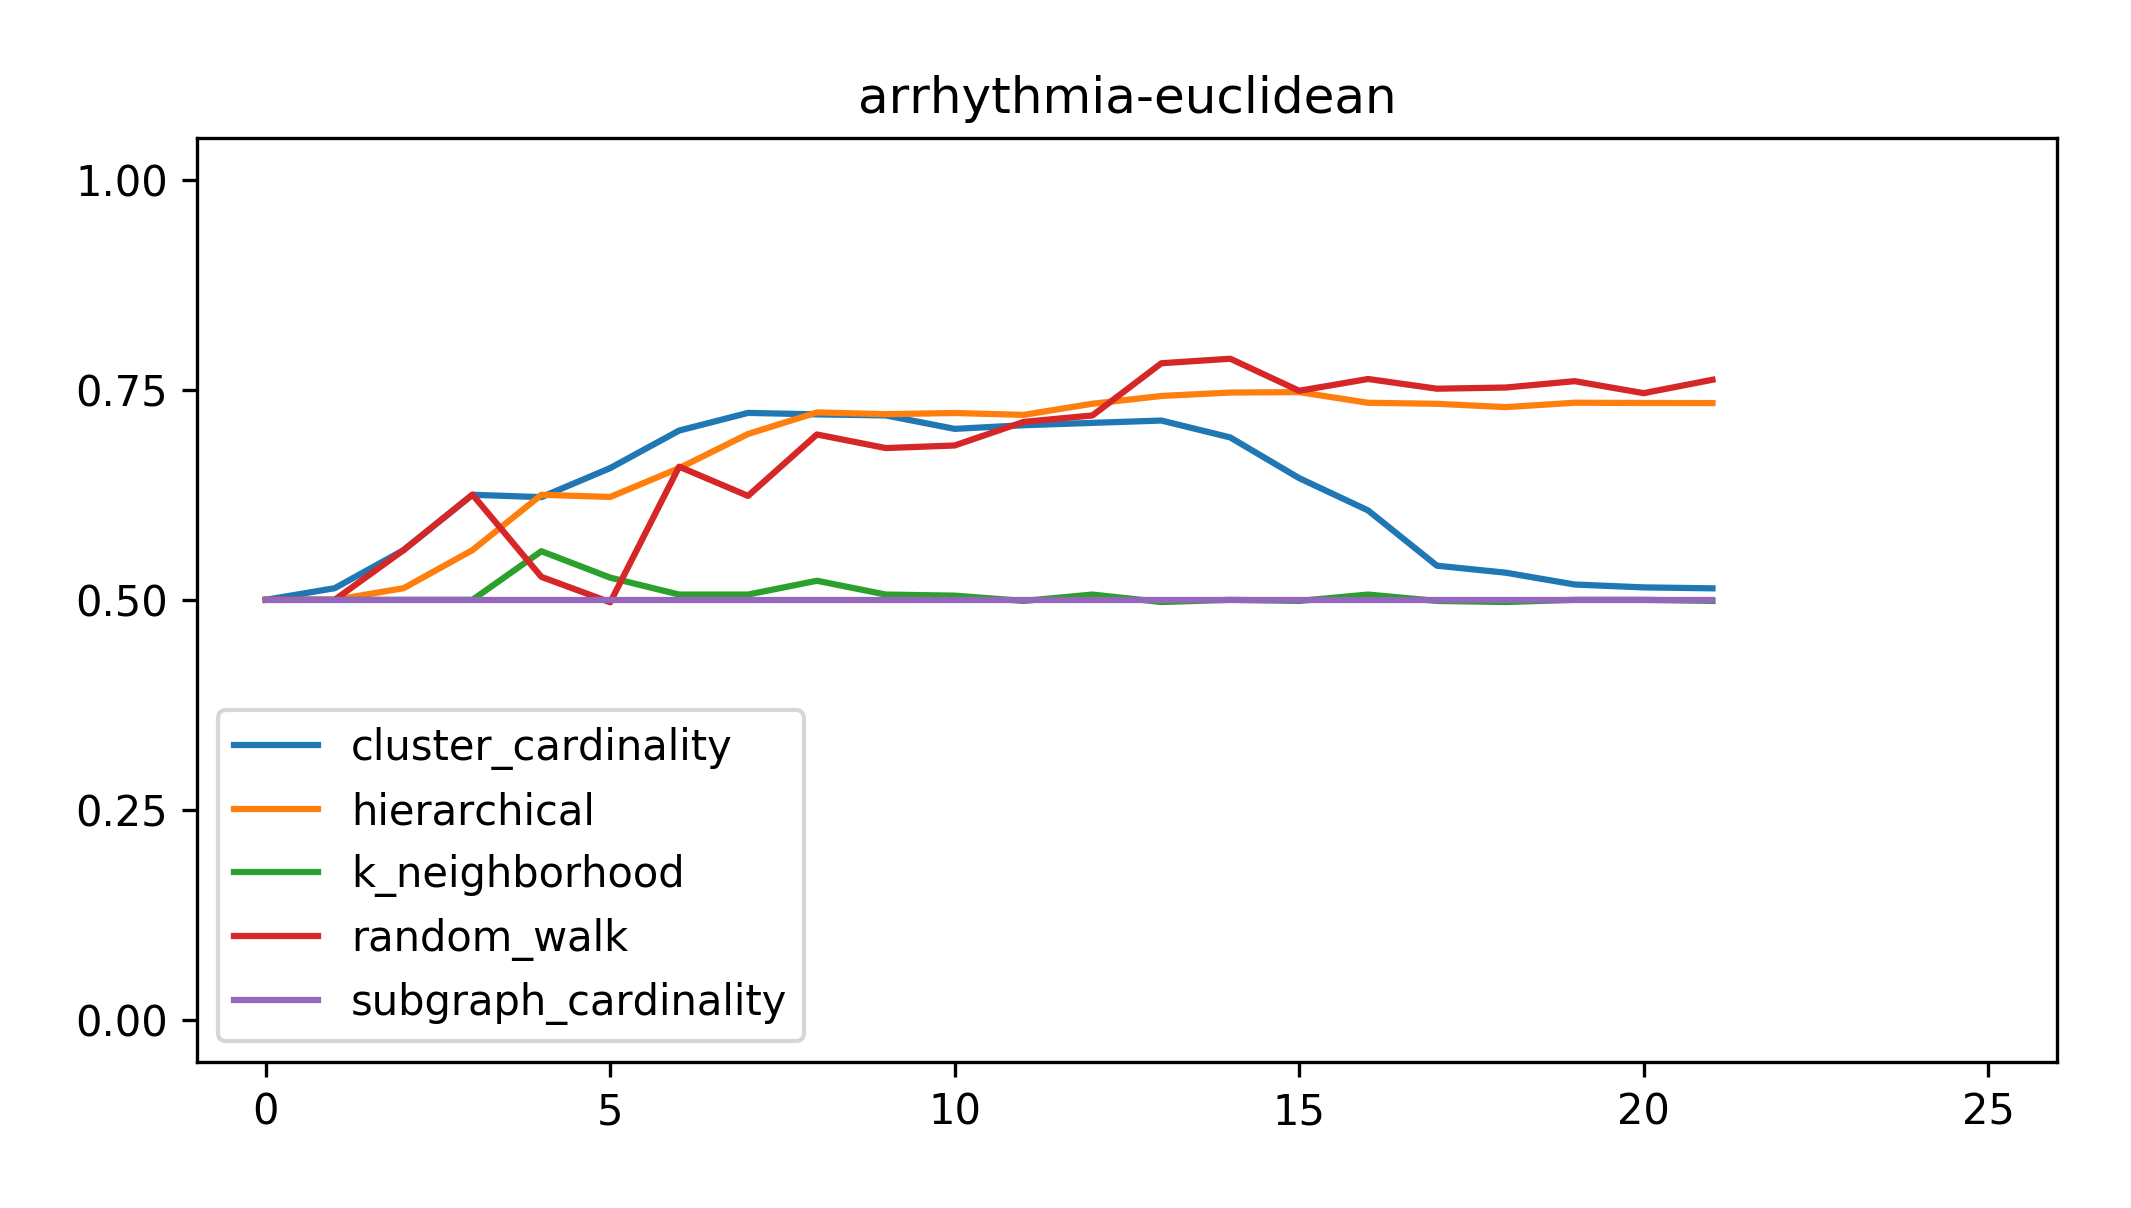
\includegraphics[width=2.2in]{kdd/static/auc_vs_depth/arrhythmia-euclidean.png}
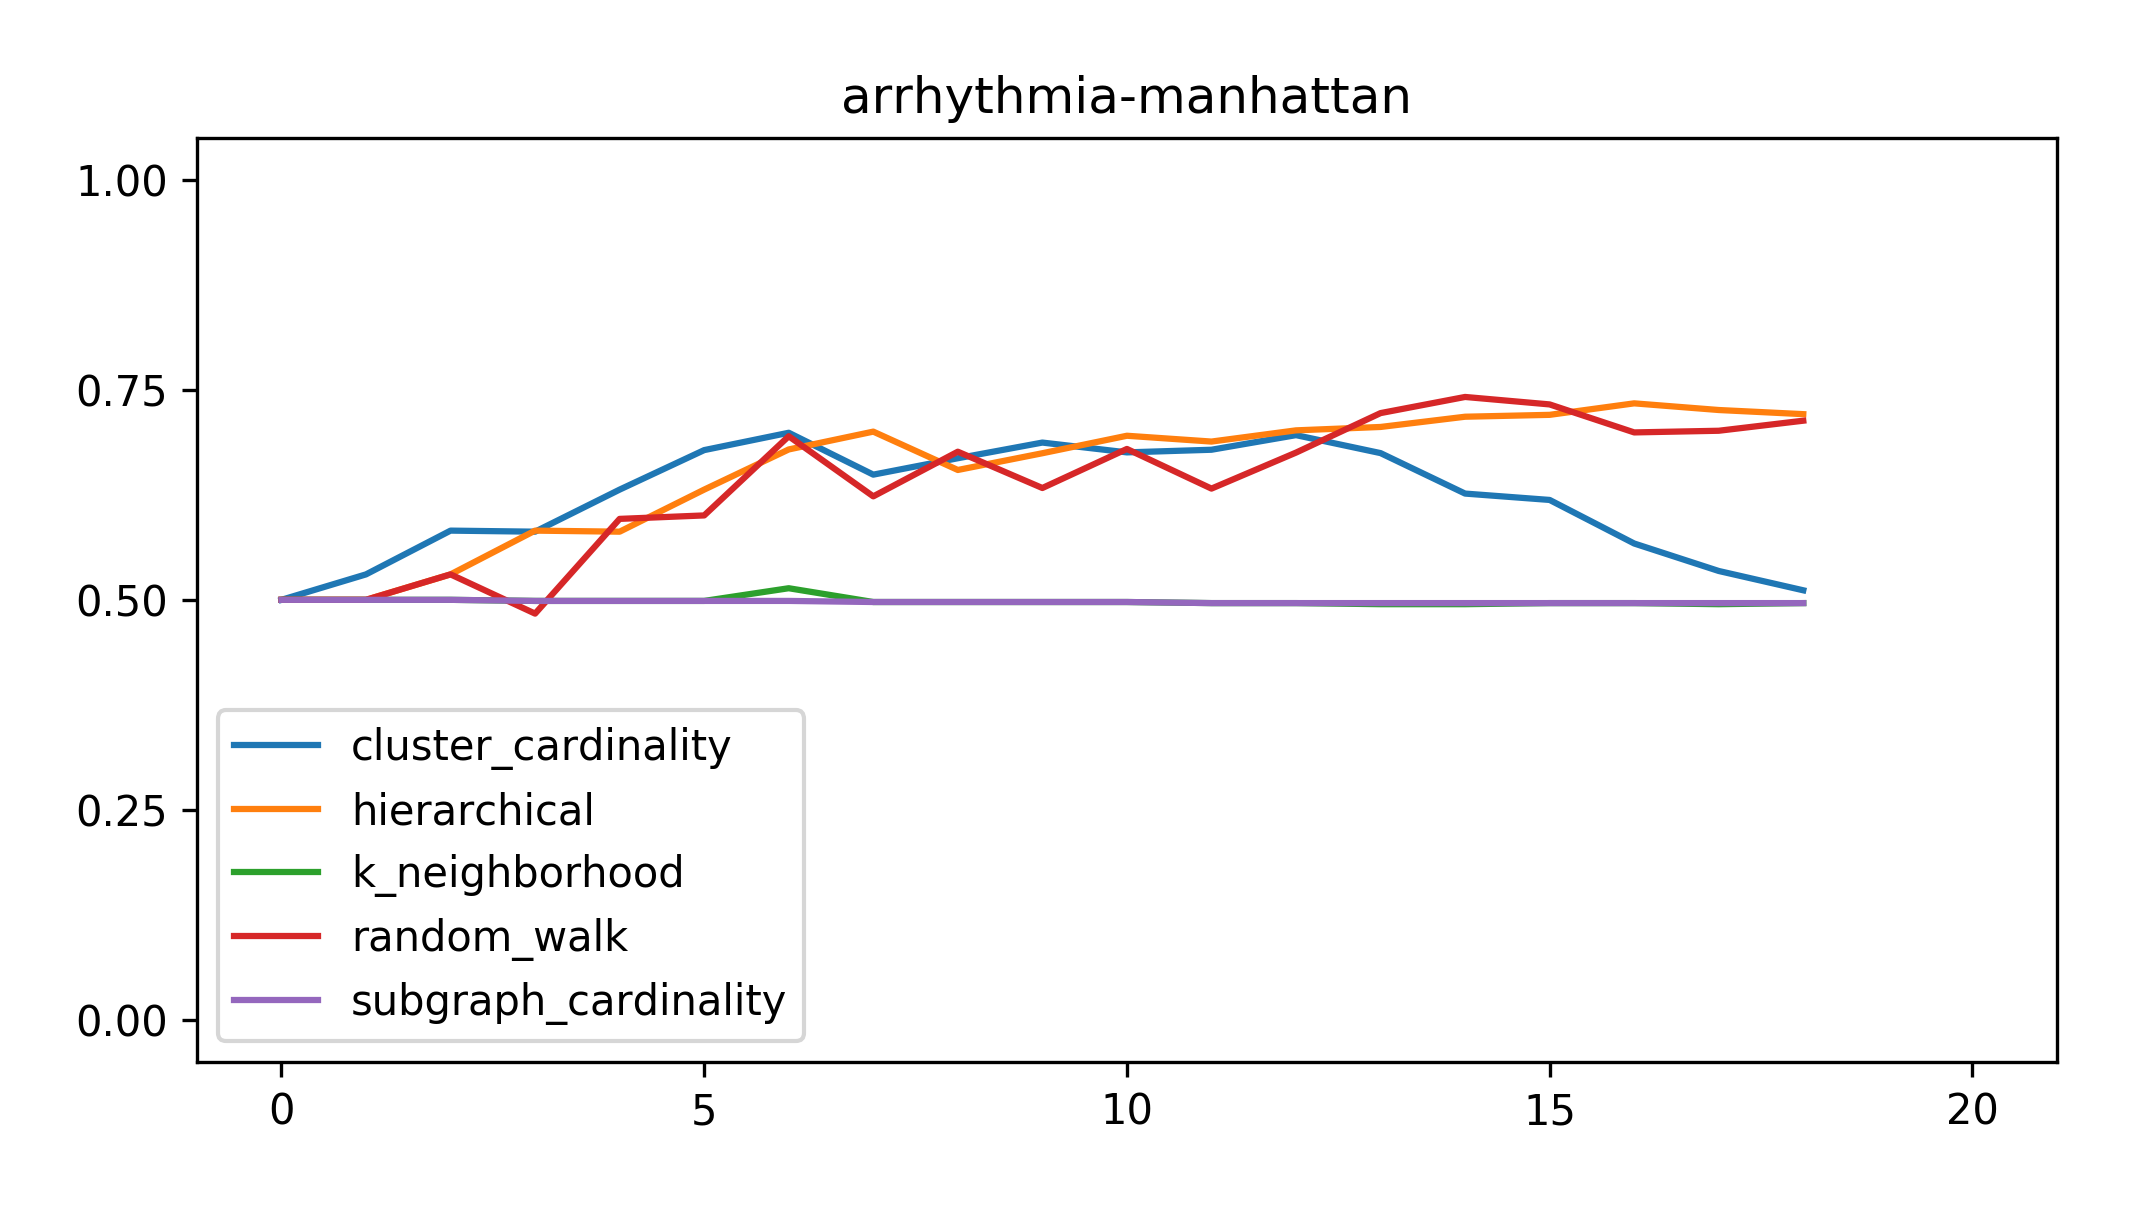
\includegraphics[width=2.2in]{kdd/static/auc_vs_depth/arrhythmia-manhattan.png}

% BreastW
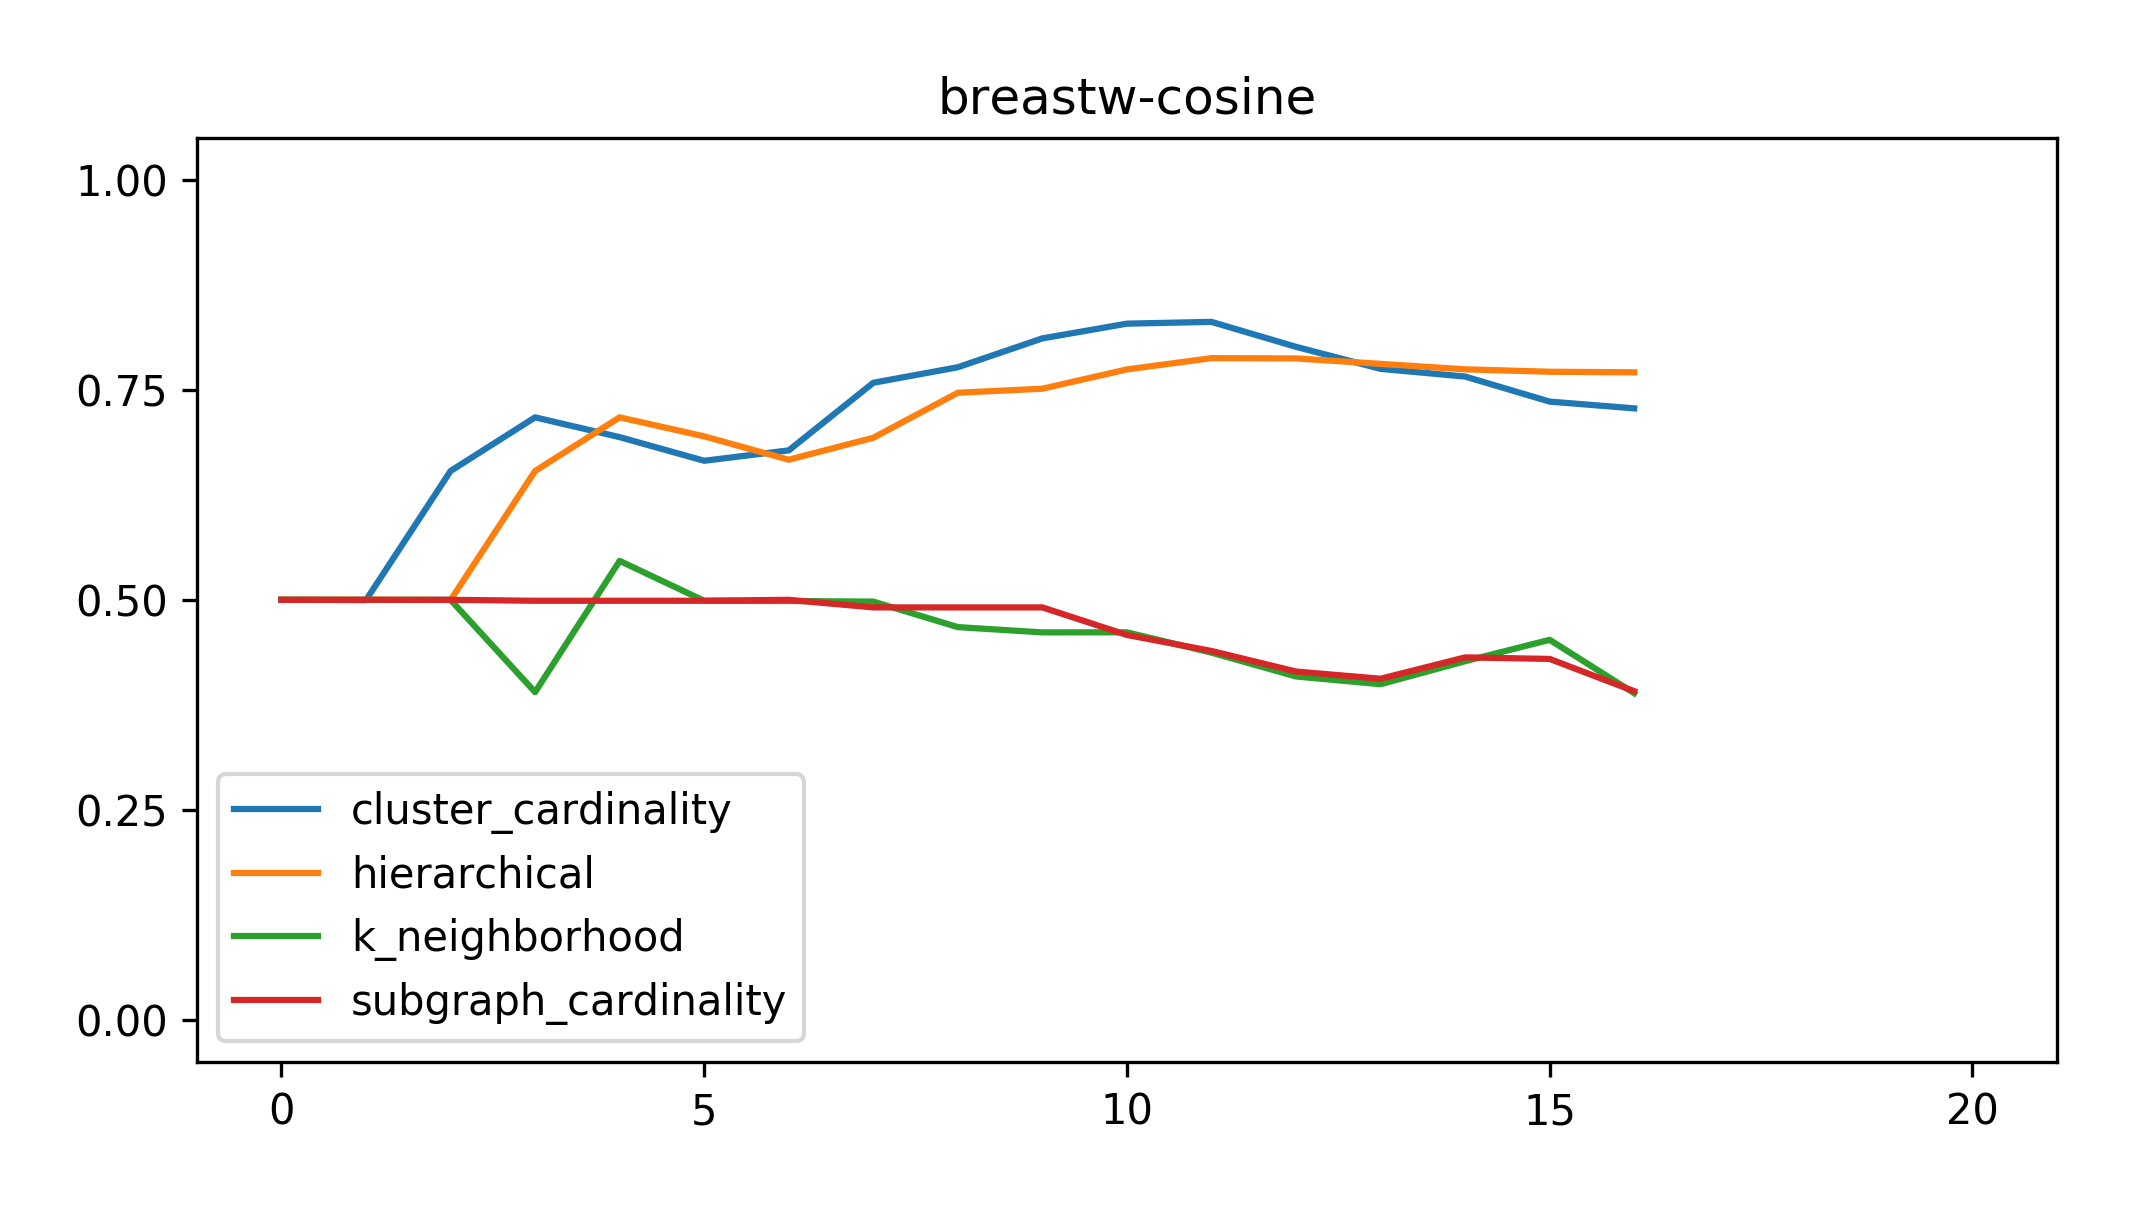
\includegraphics[width=2.2in]{kdd/static/auc_vs_depth/breastw-cosine.png}
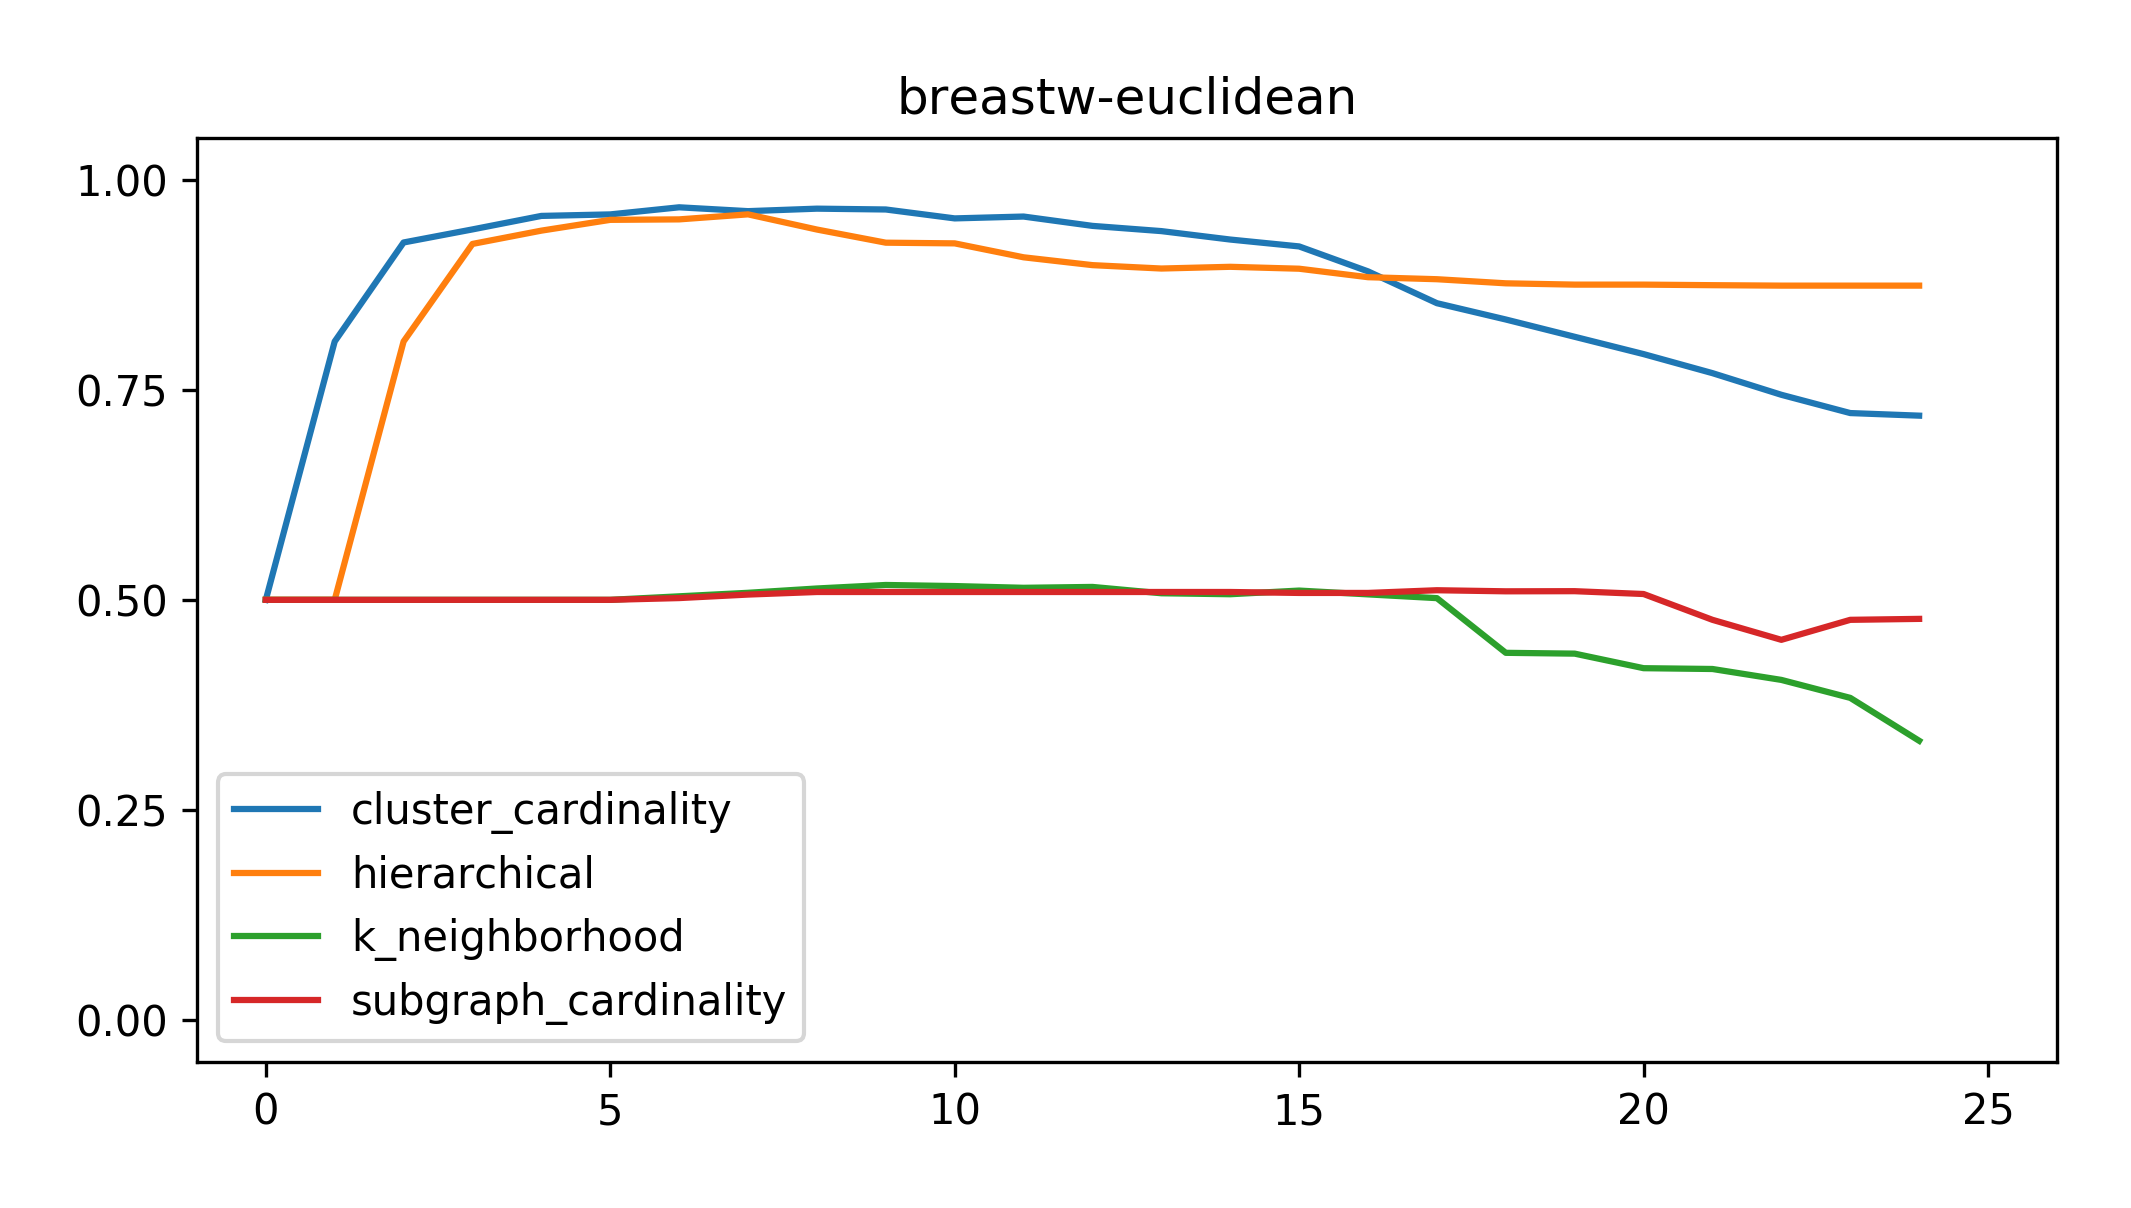
\includegraphics[width=2.2in]{kdd/static/auc_vs_depth/breastw-euclidean.png}
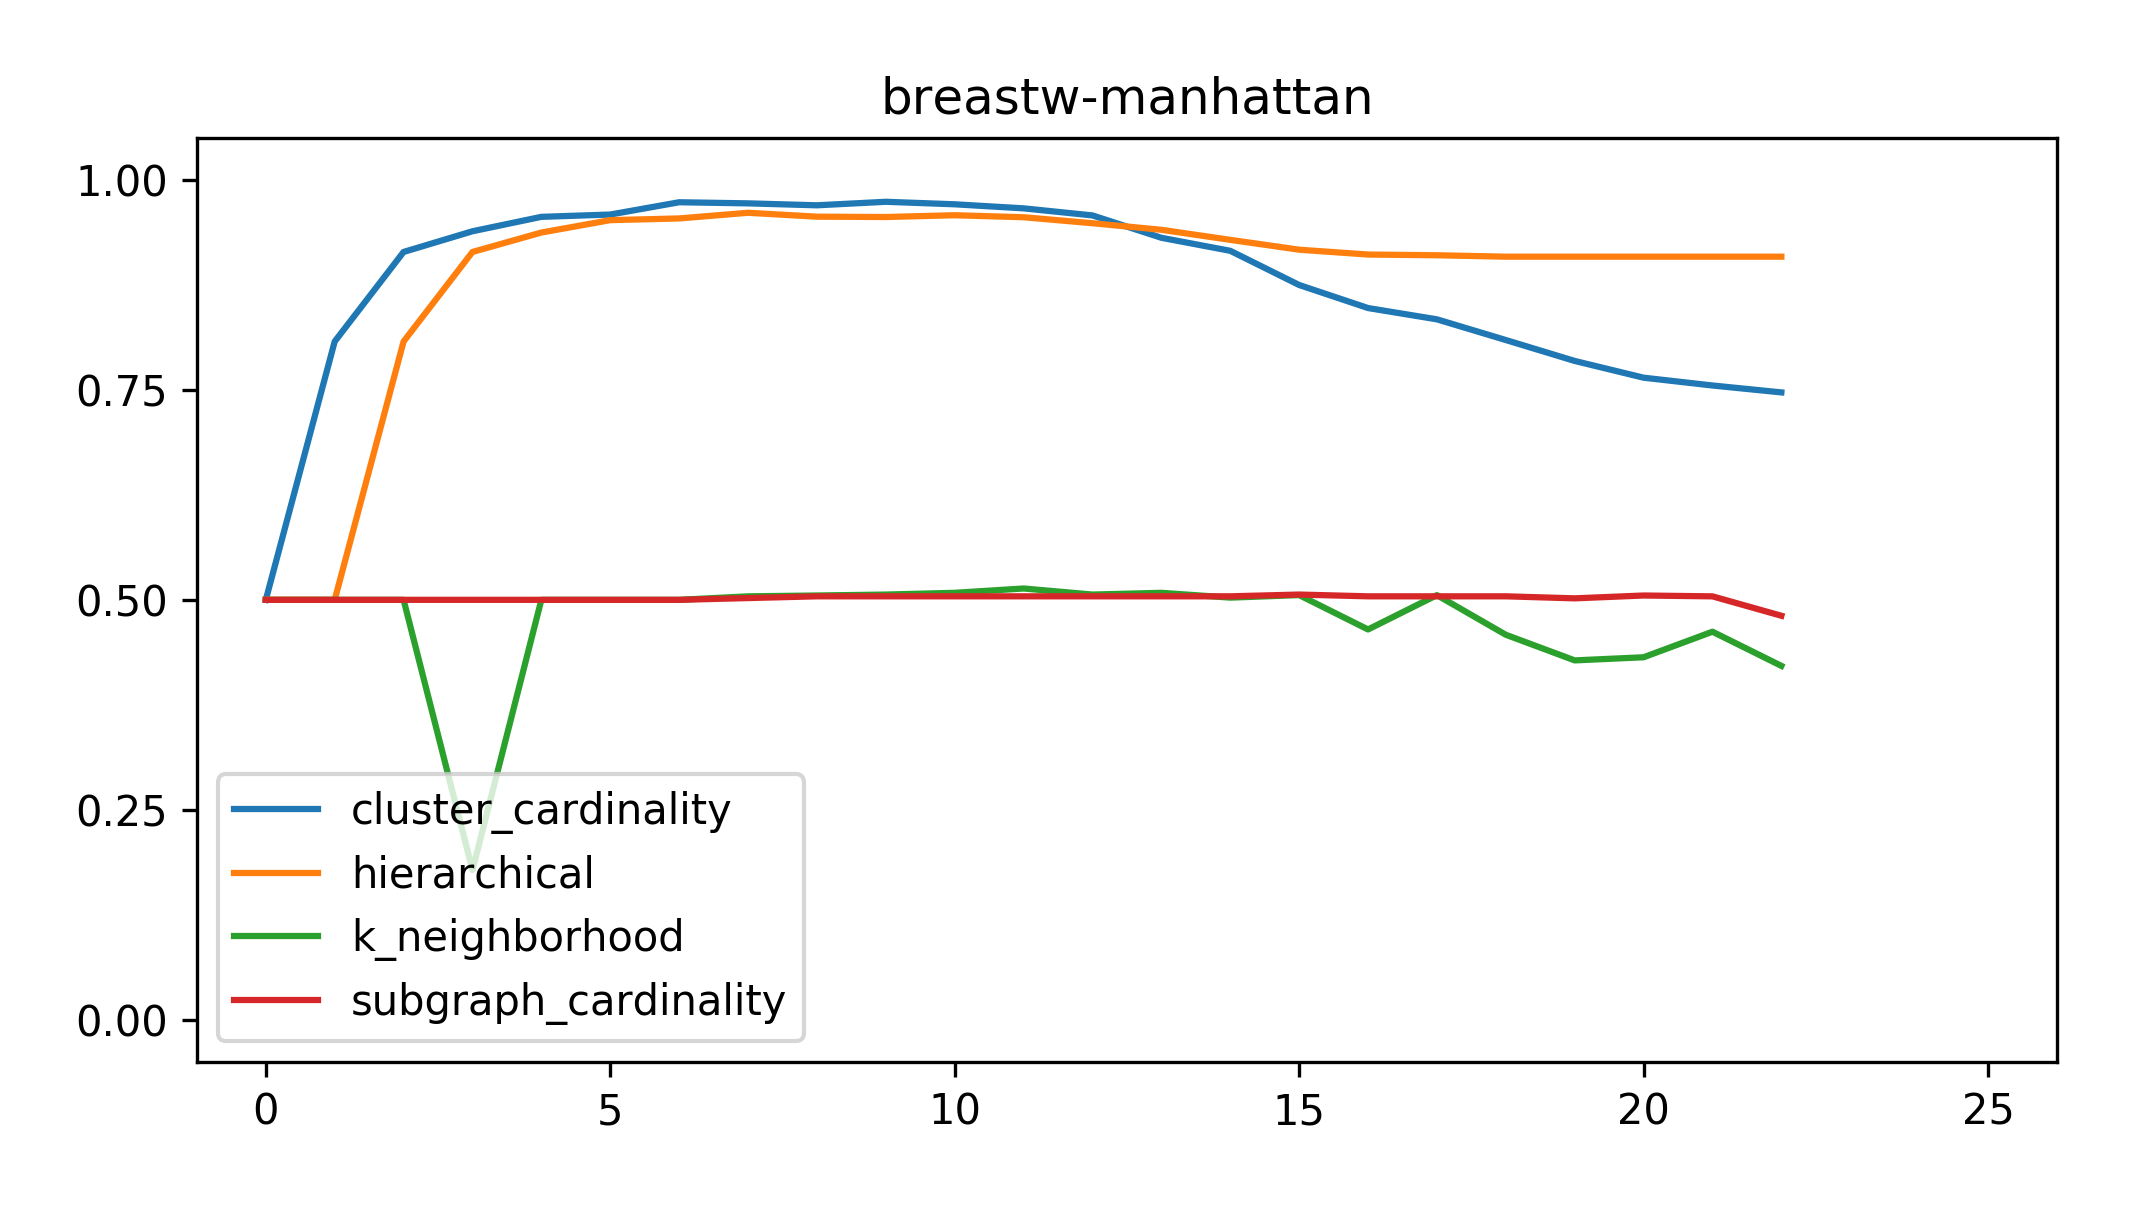
\includegraphics[width=2.2in]{kdd/static/auc_vs_depth/breastw-manhattan.png}

% Cardio
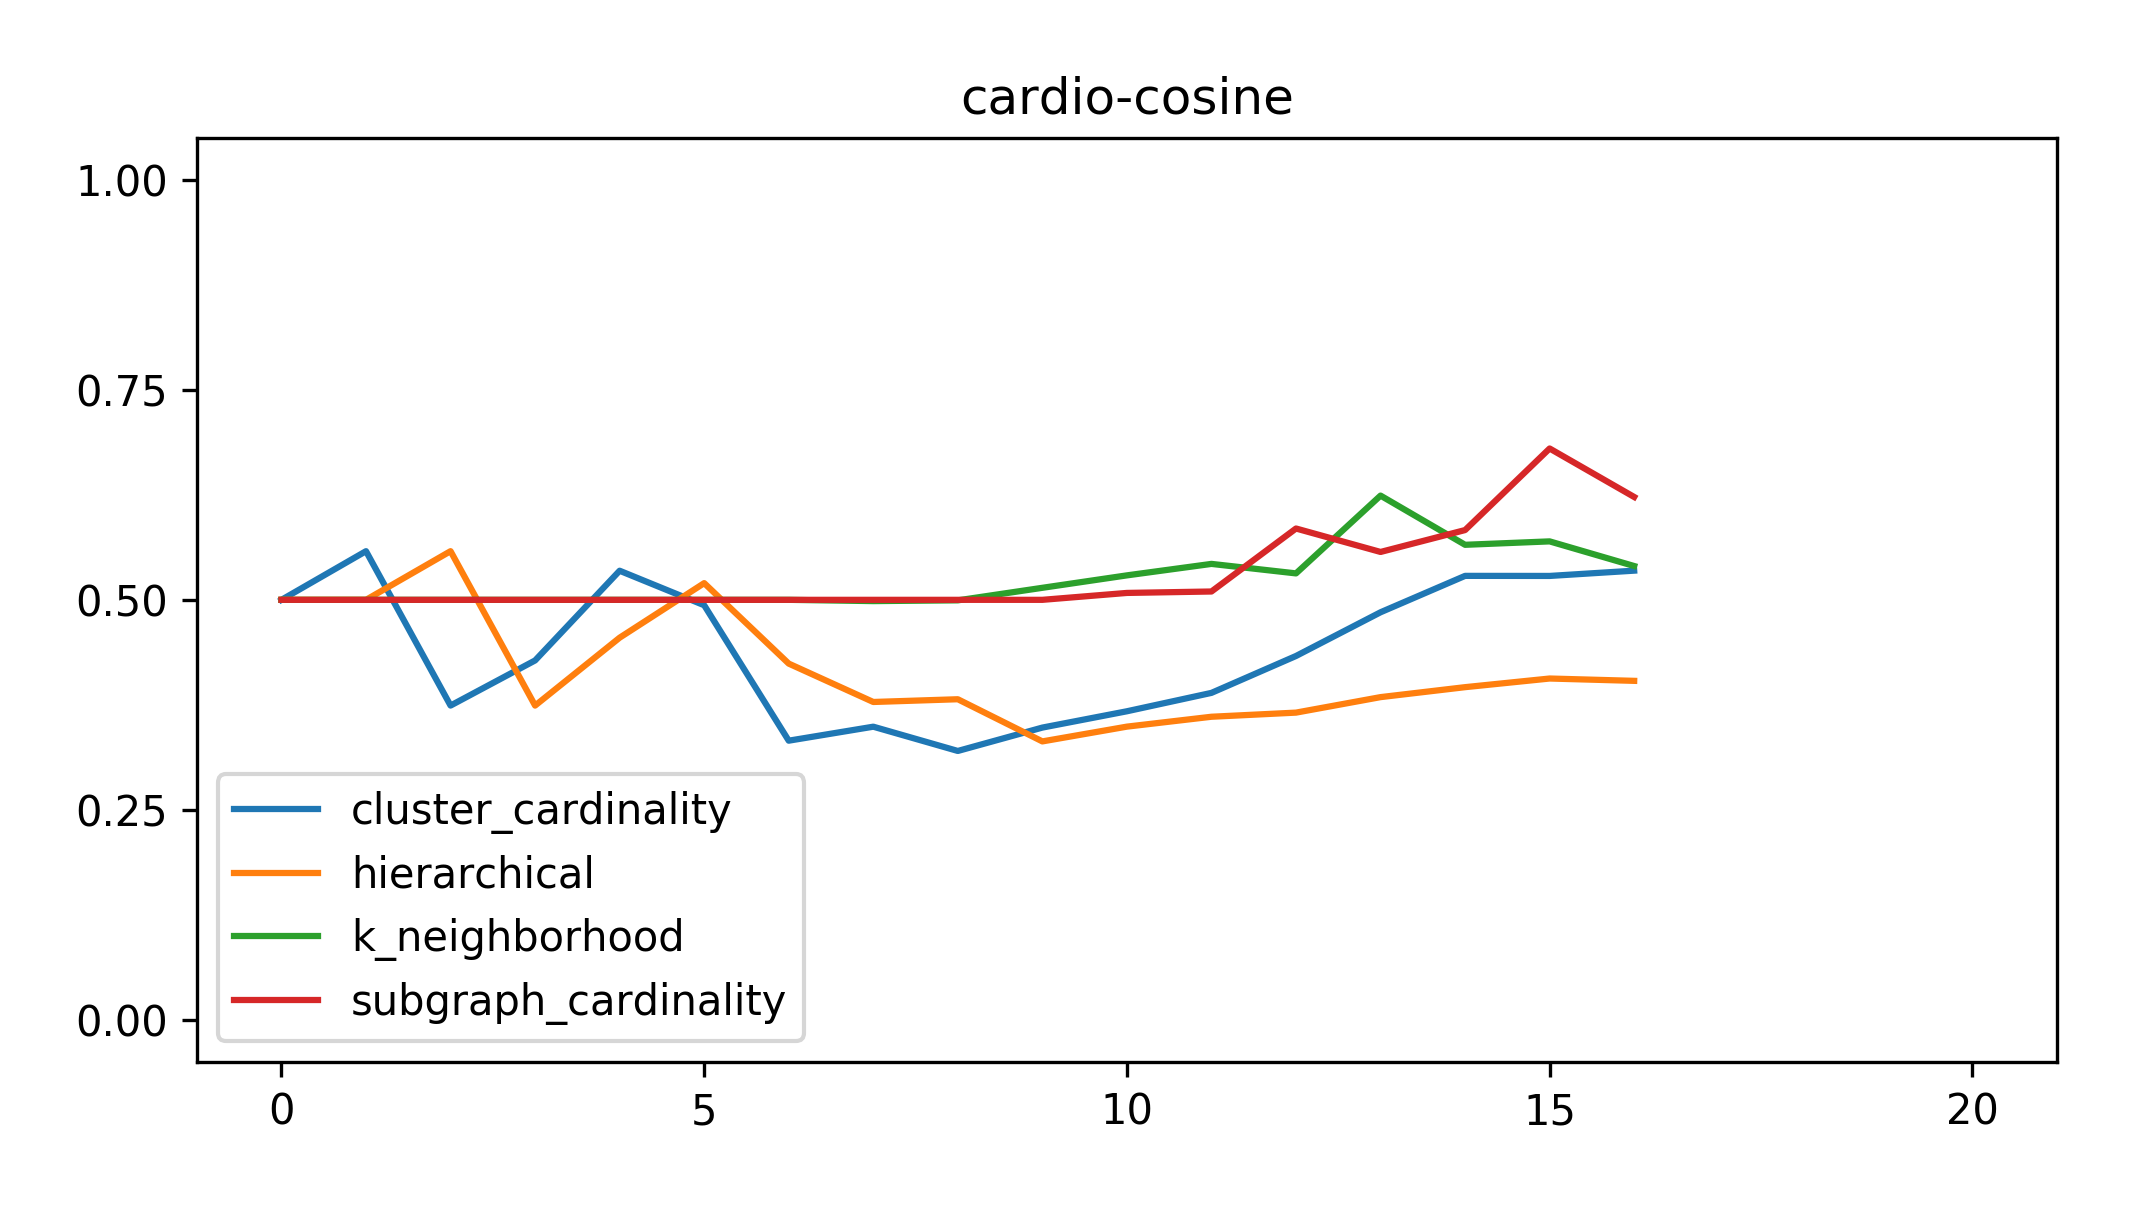
\includegraphics[width=2.2in]{kdd/static/auc_vs_depth/cardio-cosine.png}
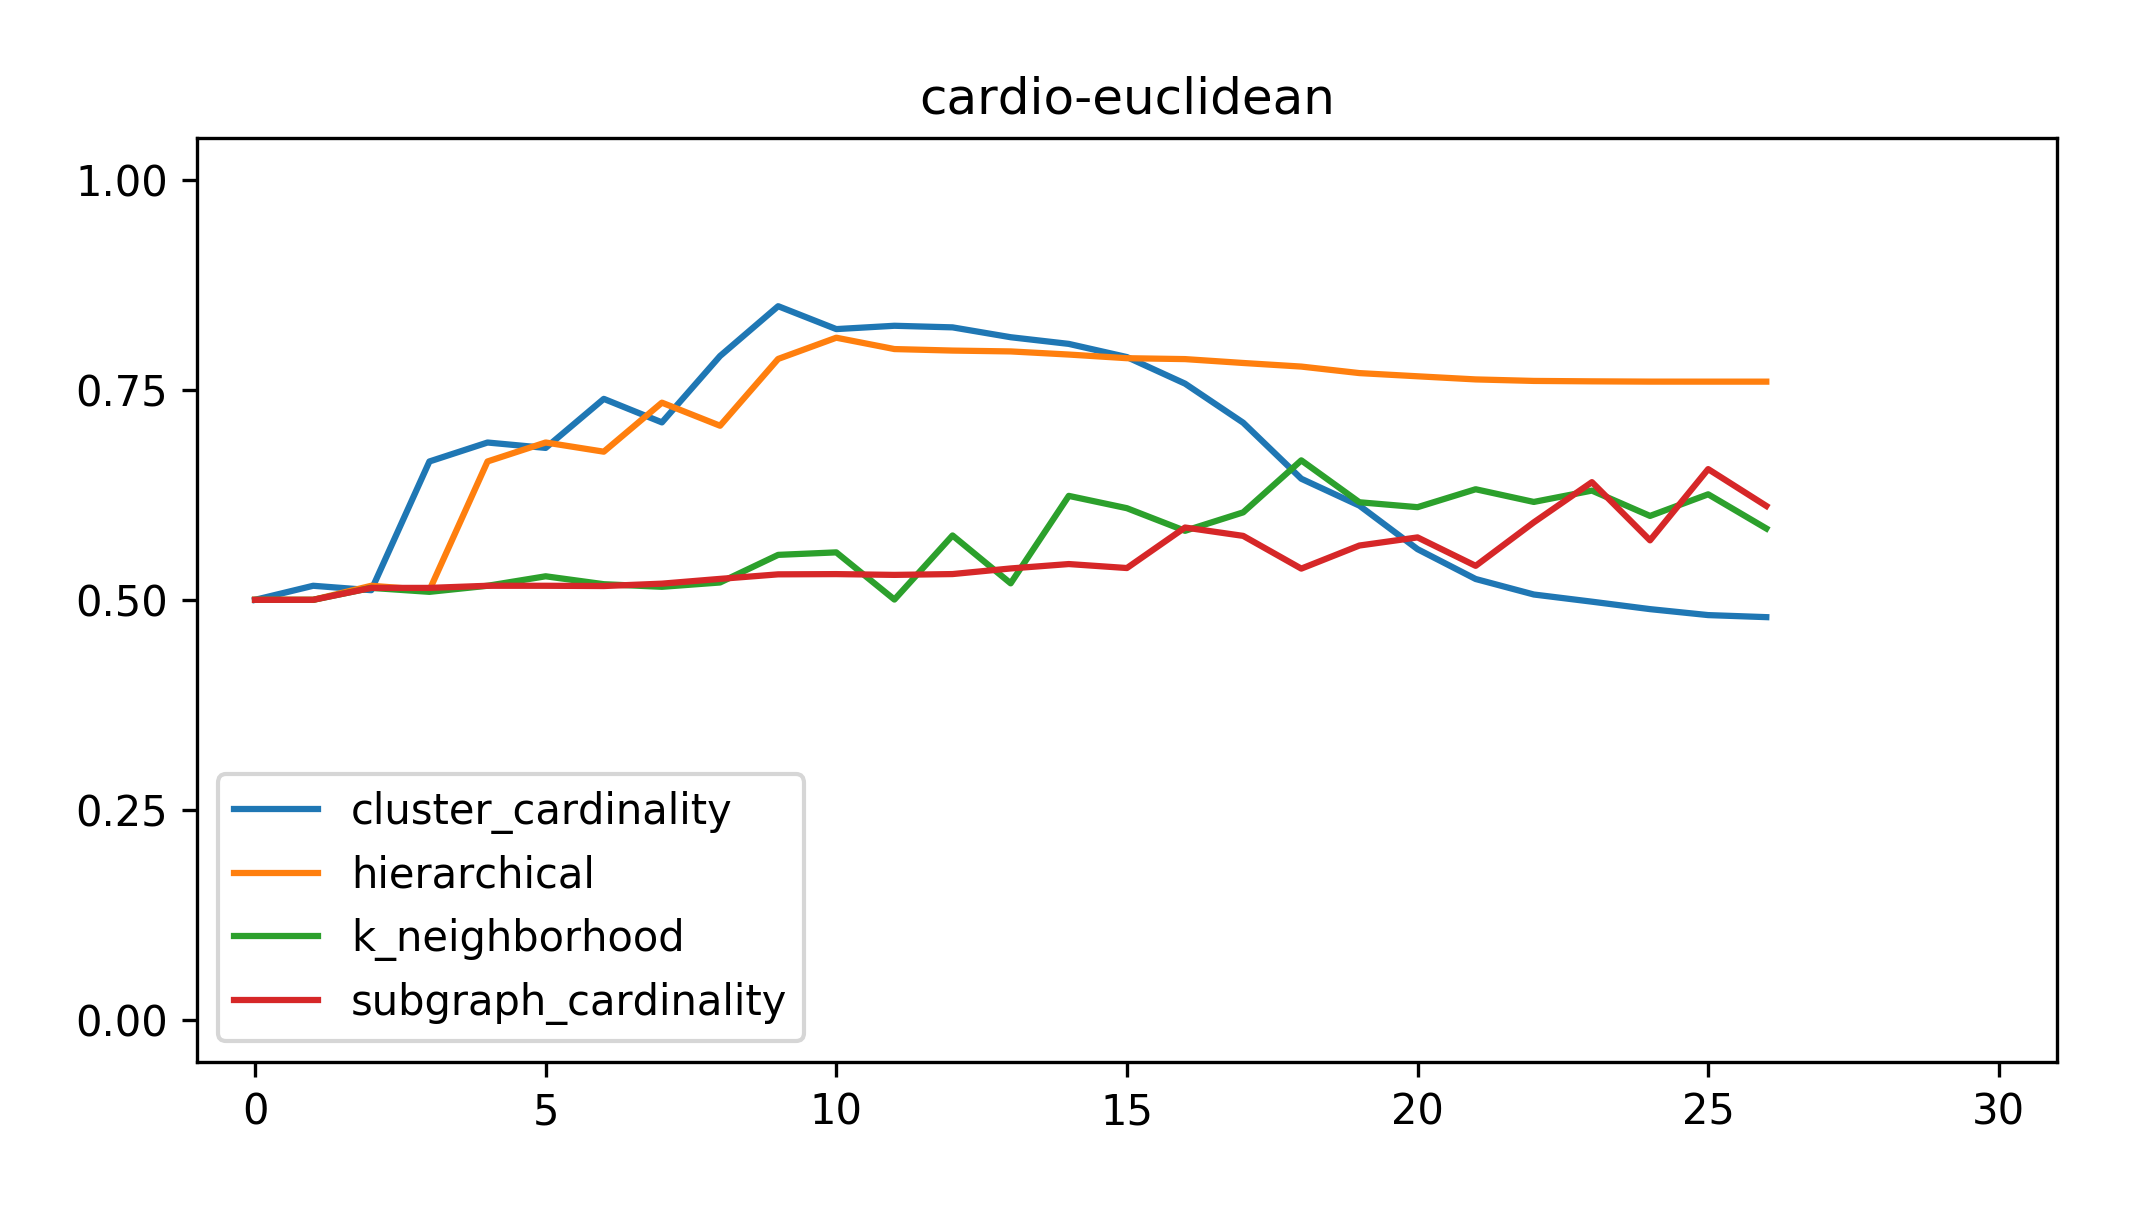
\includegraphics[width=2.2in]{kdd/static/auc_vs_depth/cardio-euclidean.png}
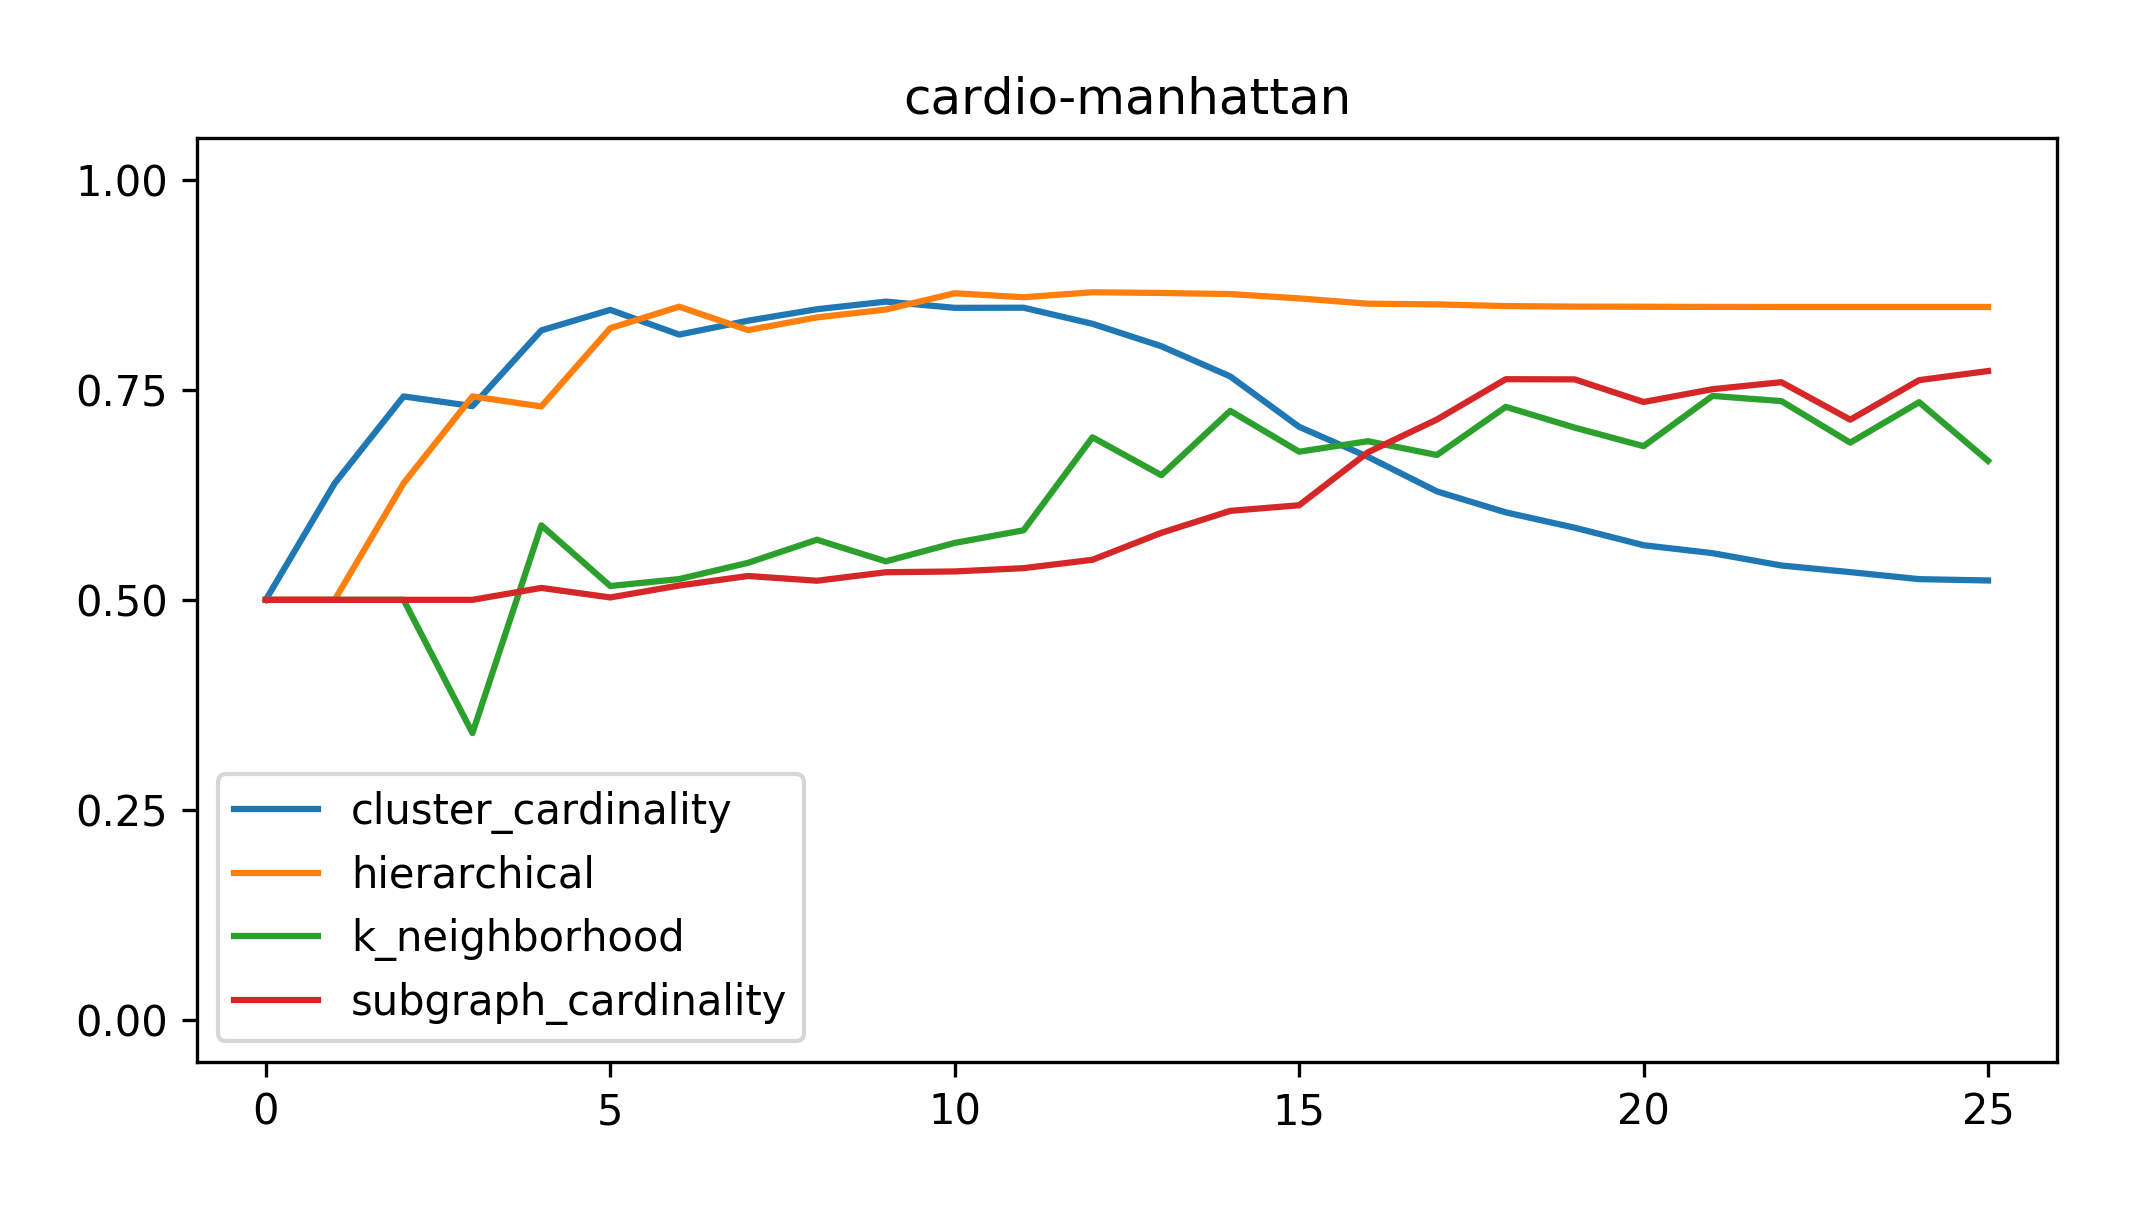
\includegraphics[width=2.2in]{kdd/static/auc_vs_depth/cardio-manhattan.png}

% Glass
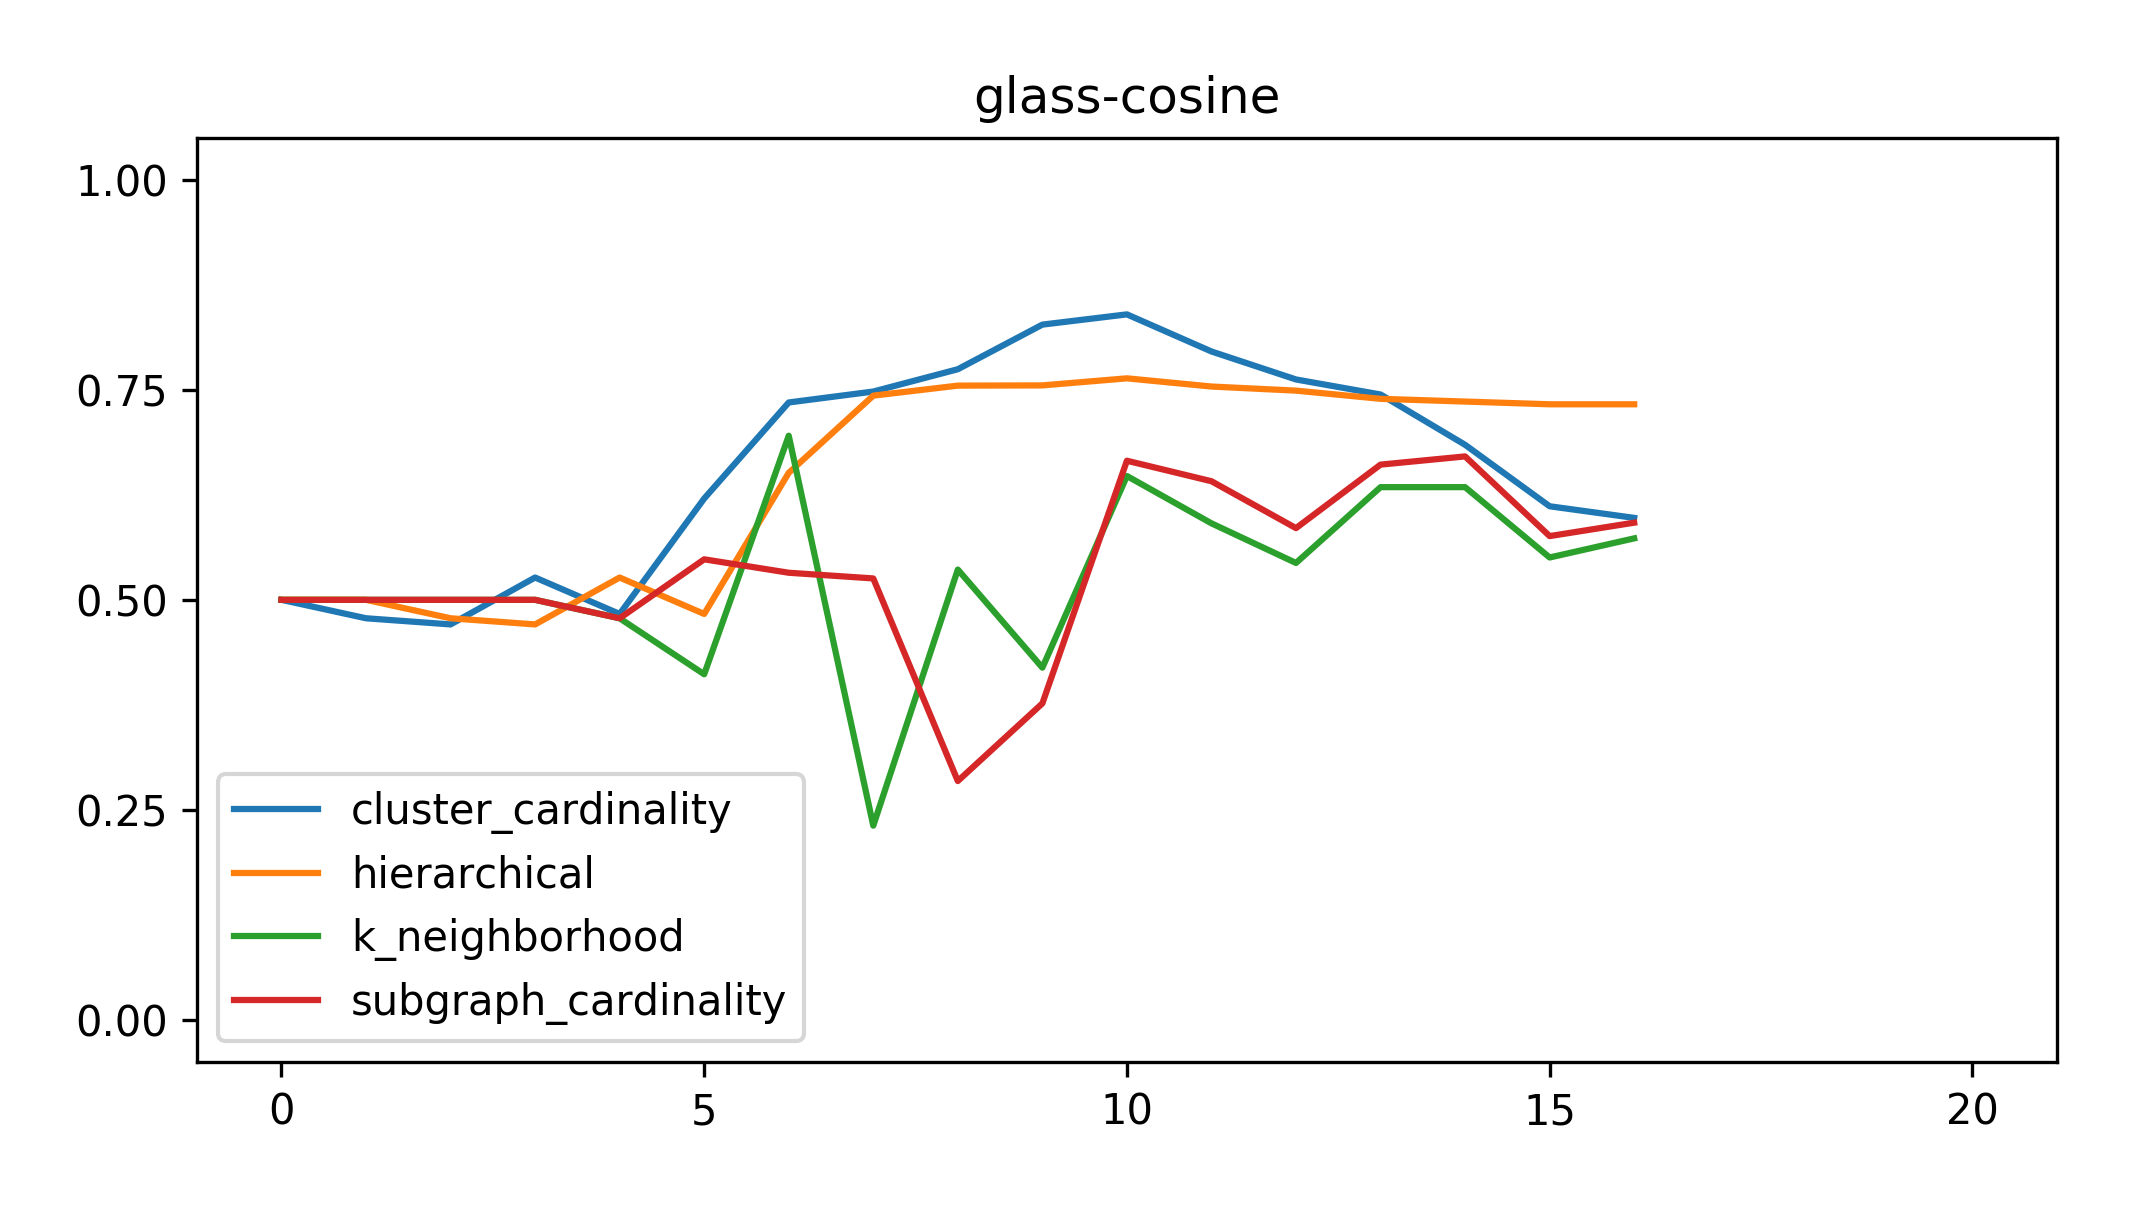
\includegraphics[width=2.2in]{kdd/static/auc_vs_depth/glass-cosine.png}
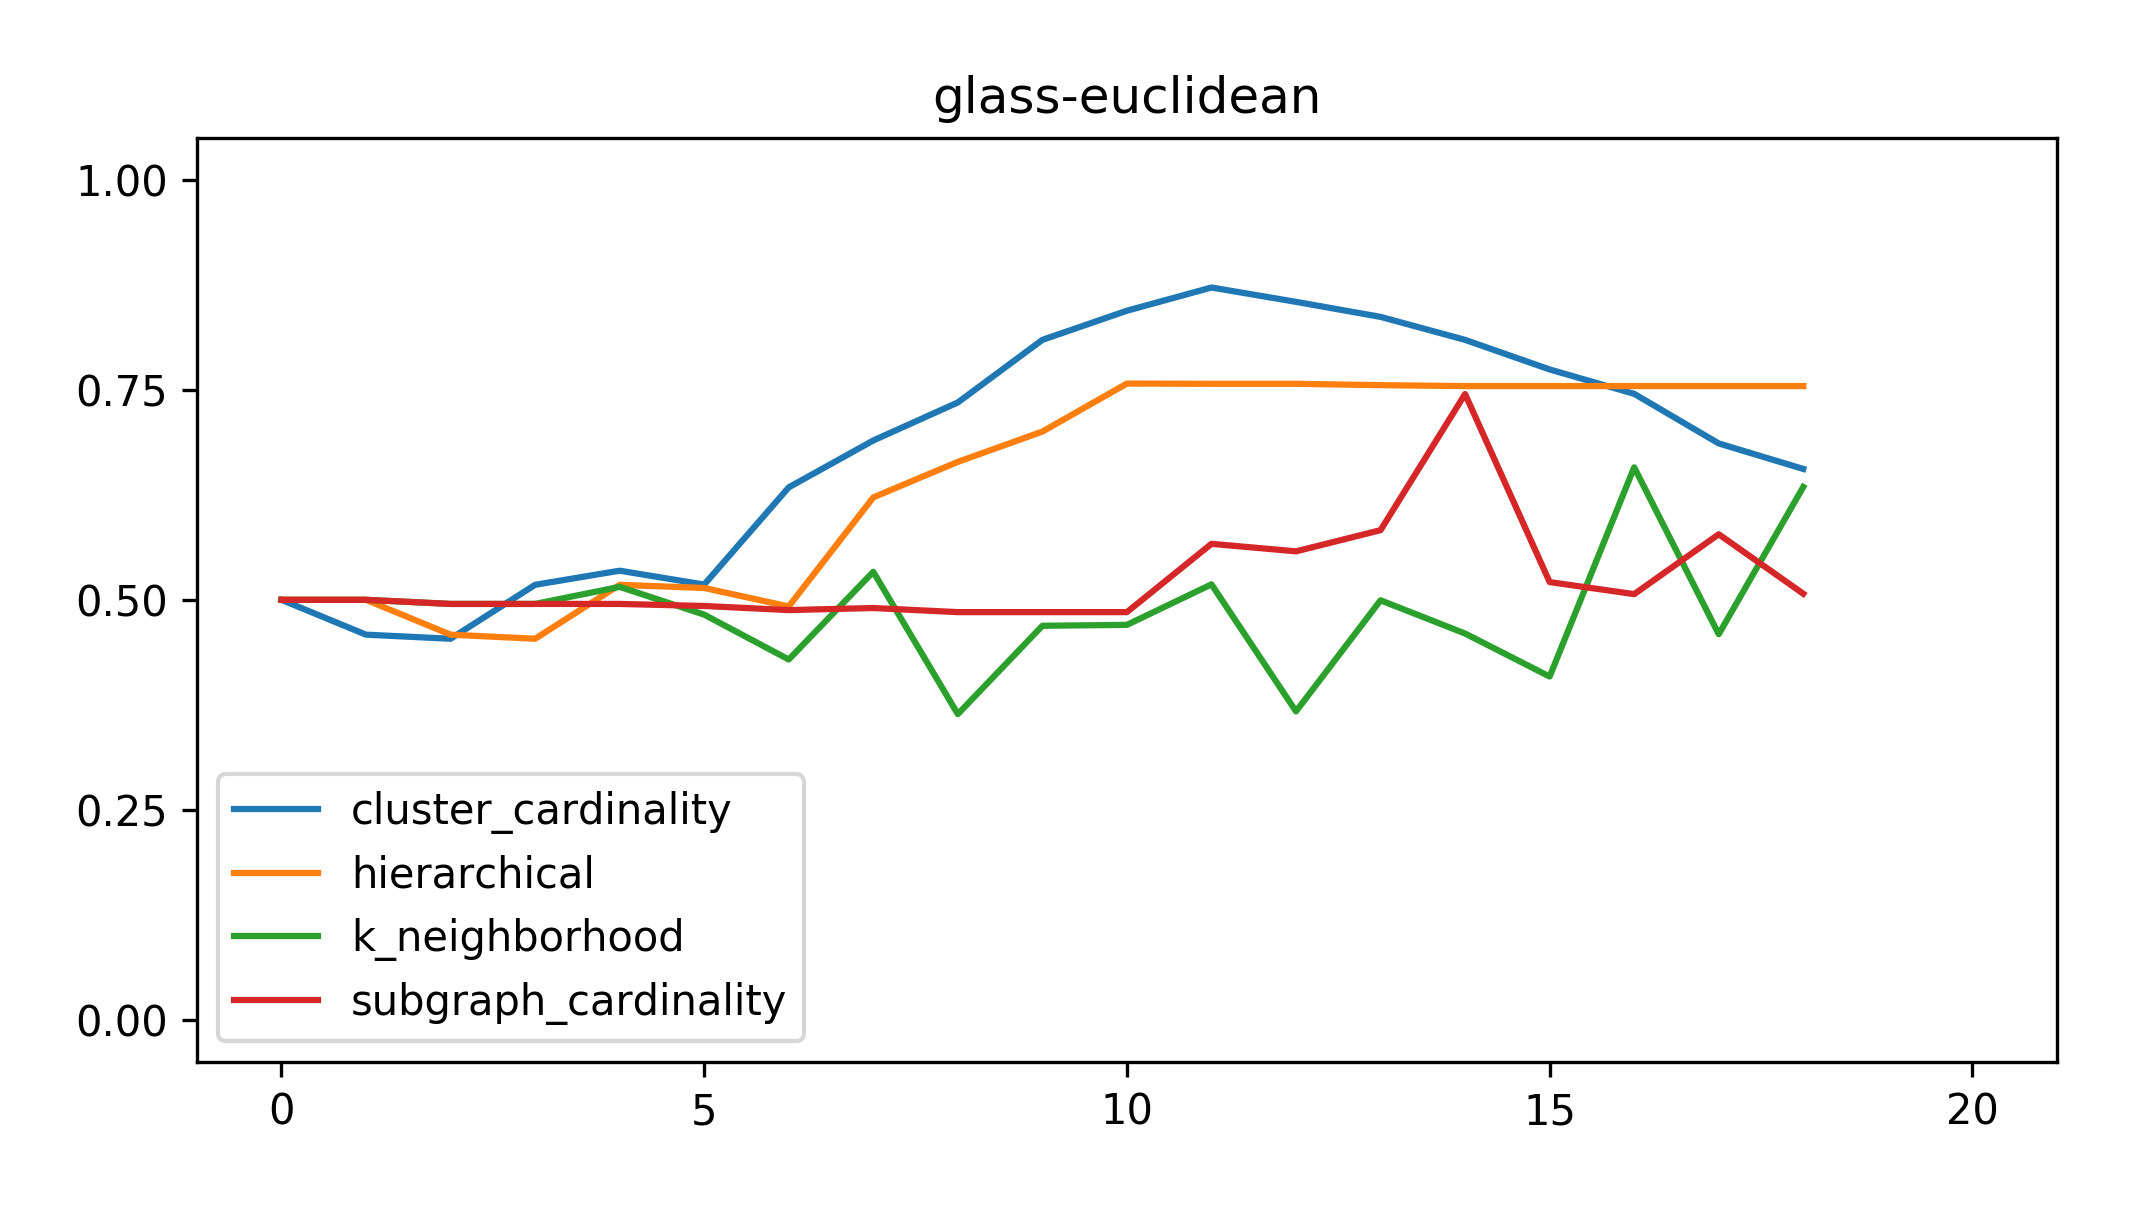
\includegraphics[width=2.2in]{kdd/static/auc_vs_depth/glass-euclidean.png}
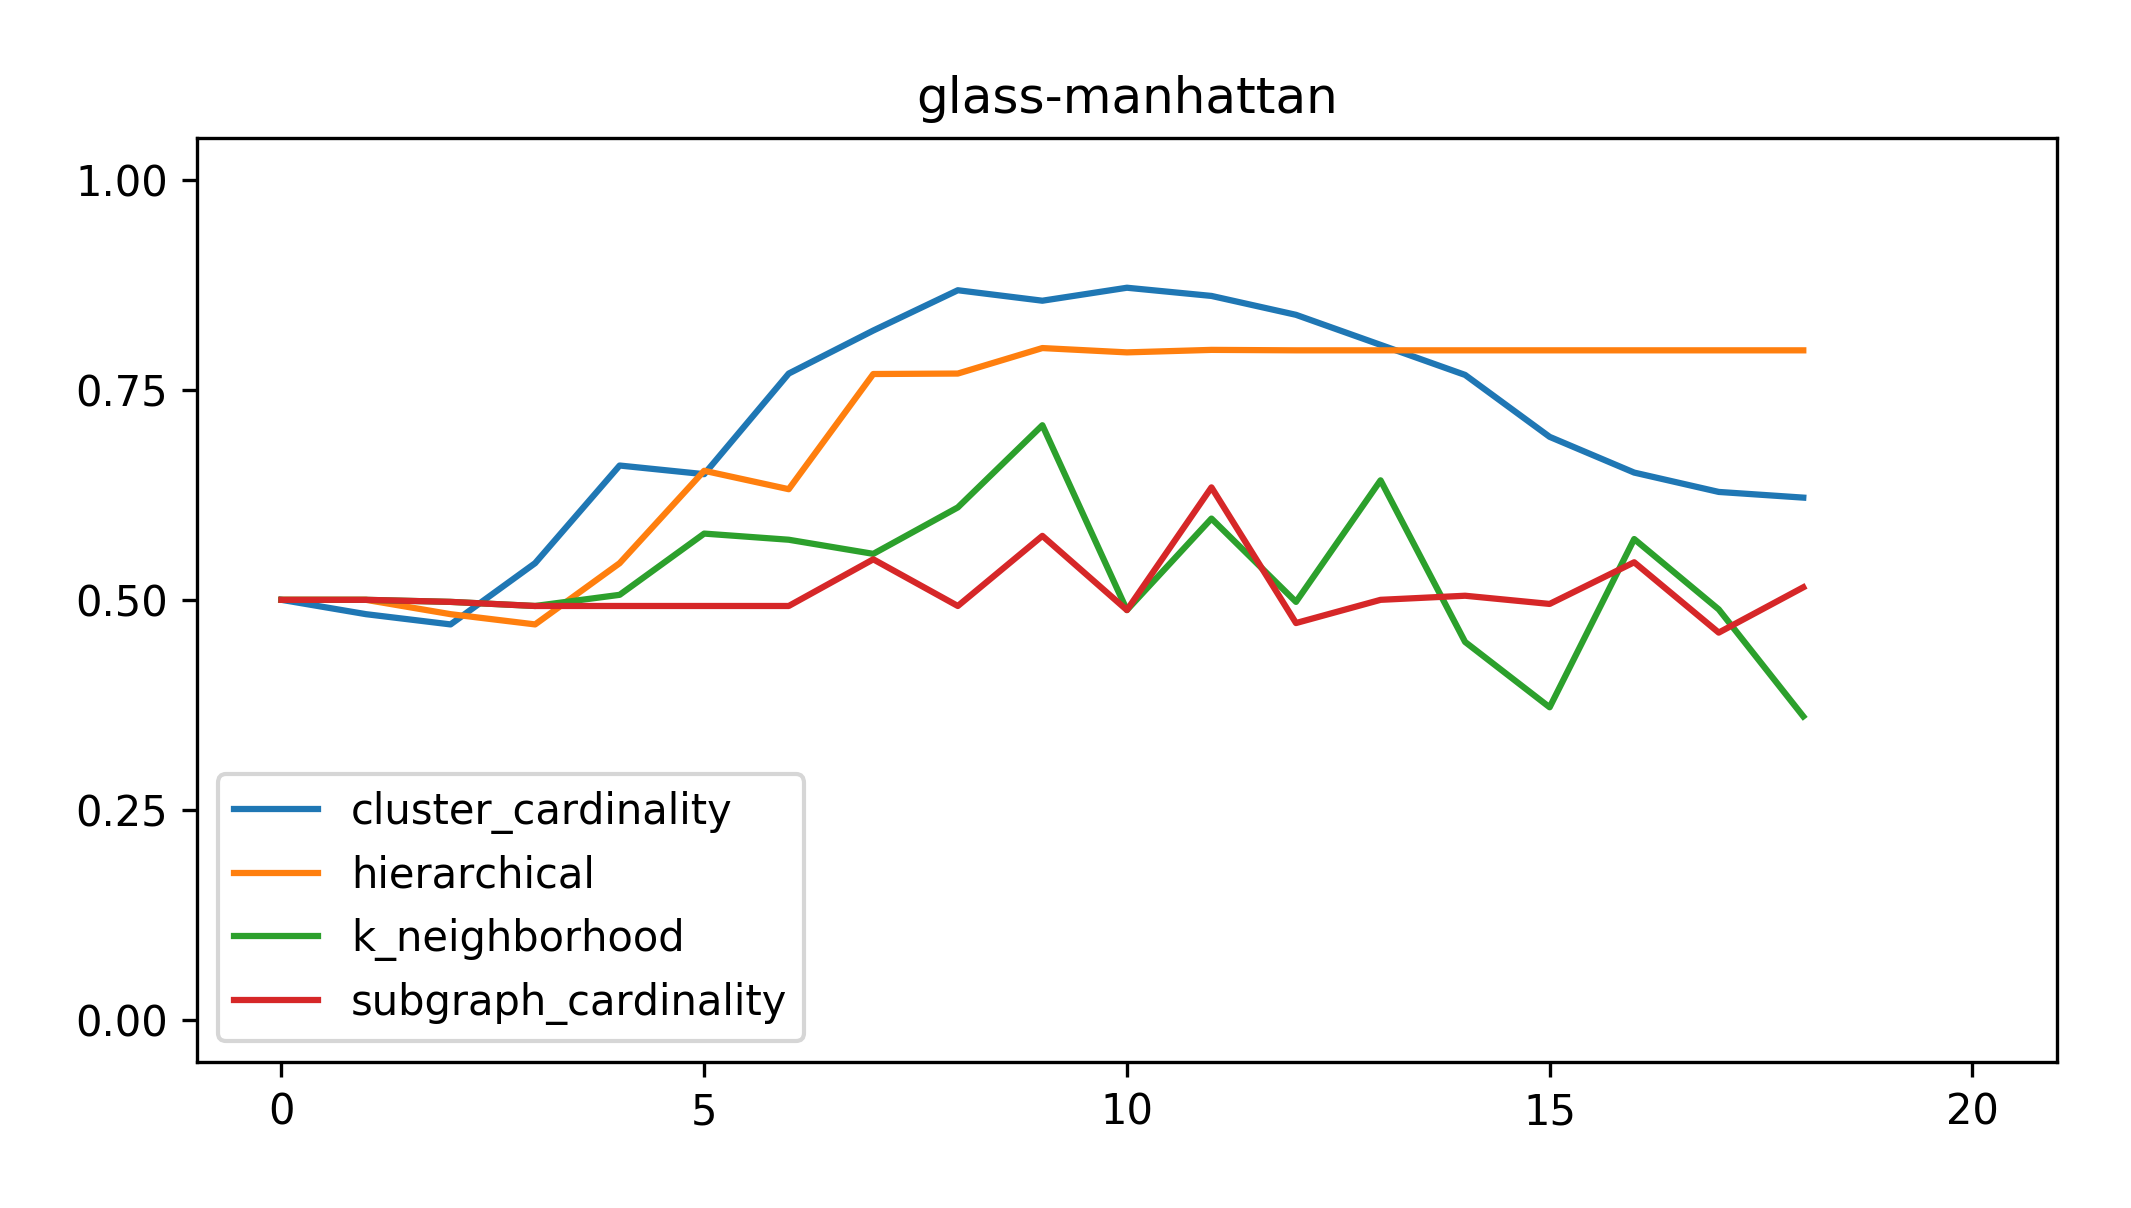
\includegraphics[width=2.2in]{kdd/static/auc_vs_depth/glass-manhattan.png}

% Ionosphere
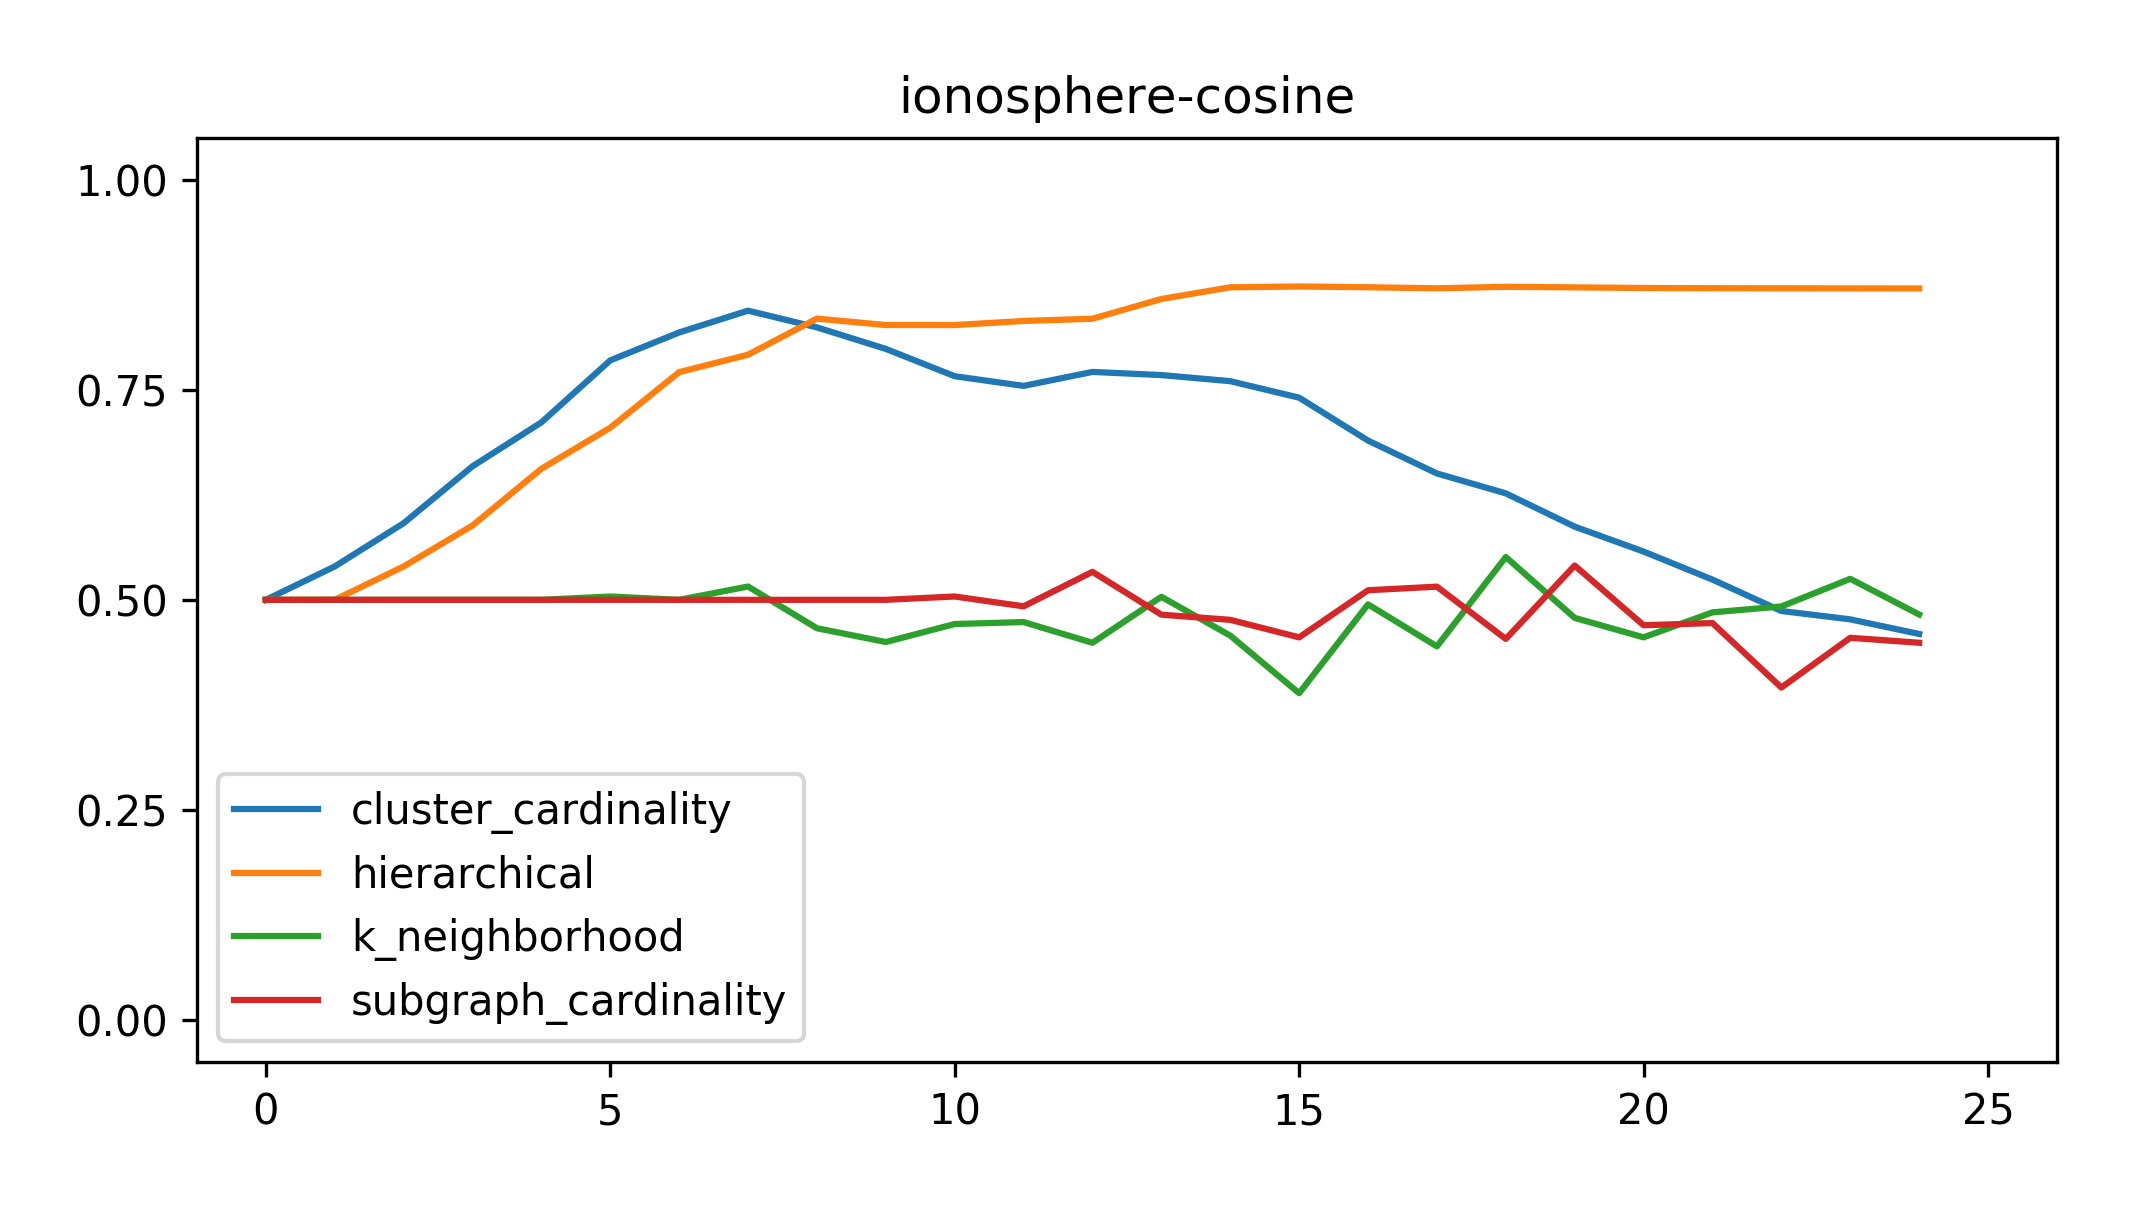
\includegraphics[width=2.2in]{kdd/static/auc_vs_depth/ionosphere-cosine.png}
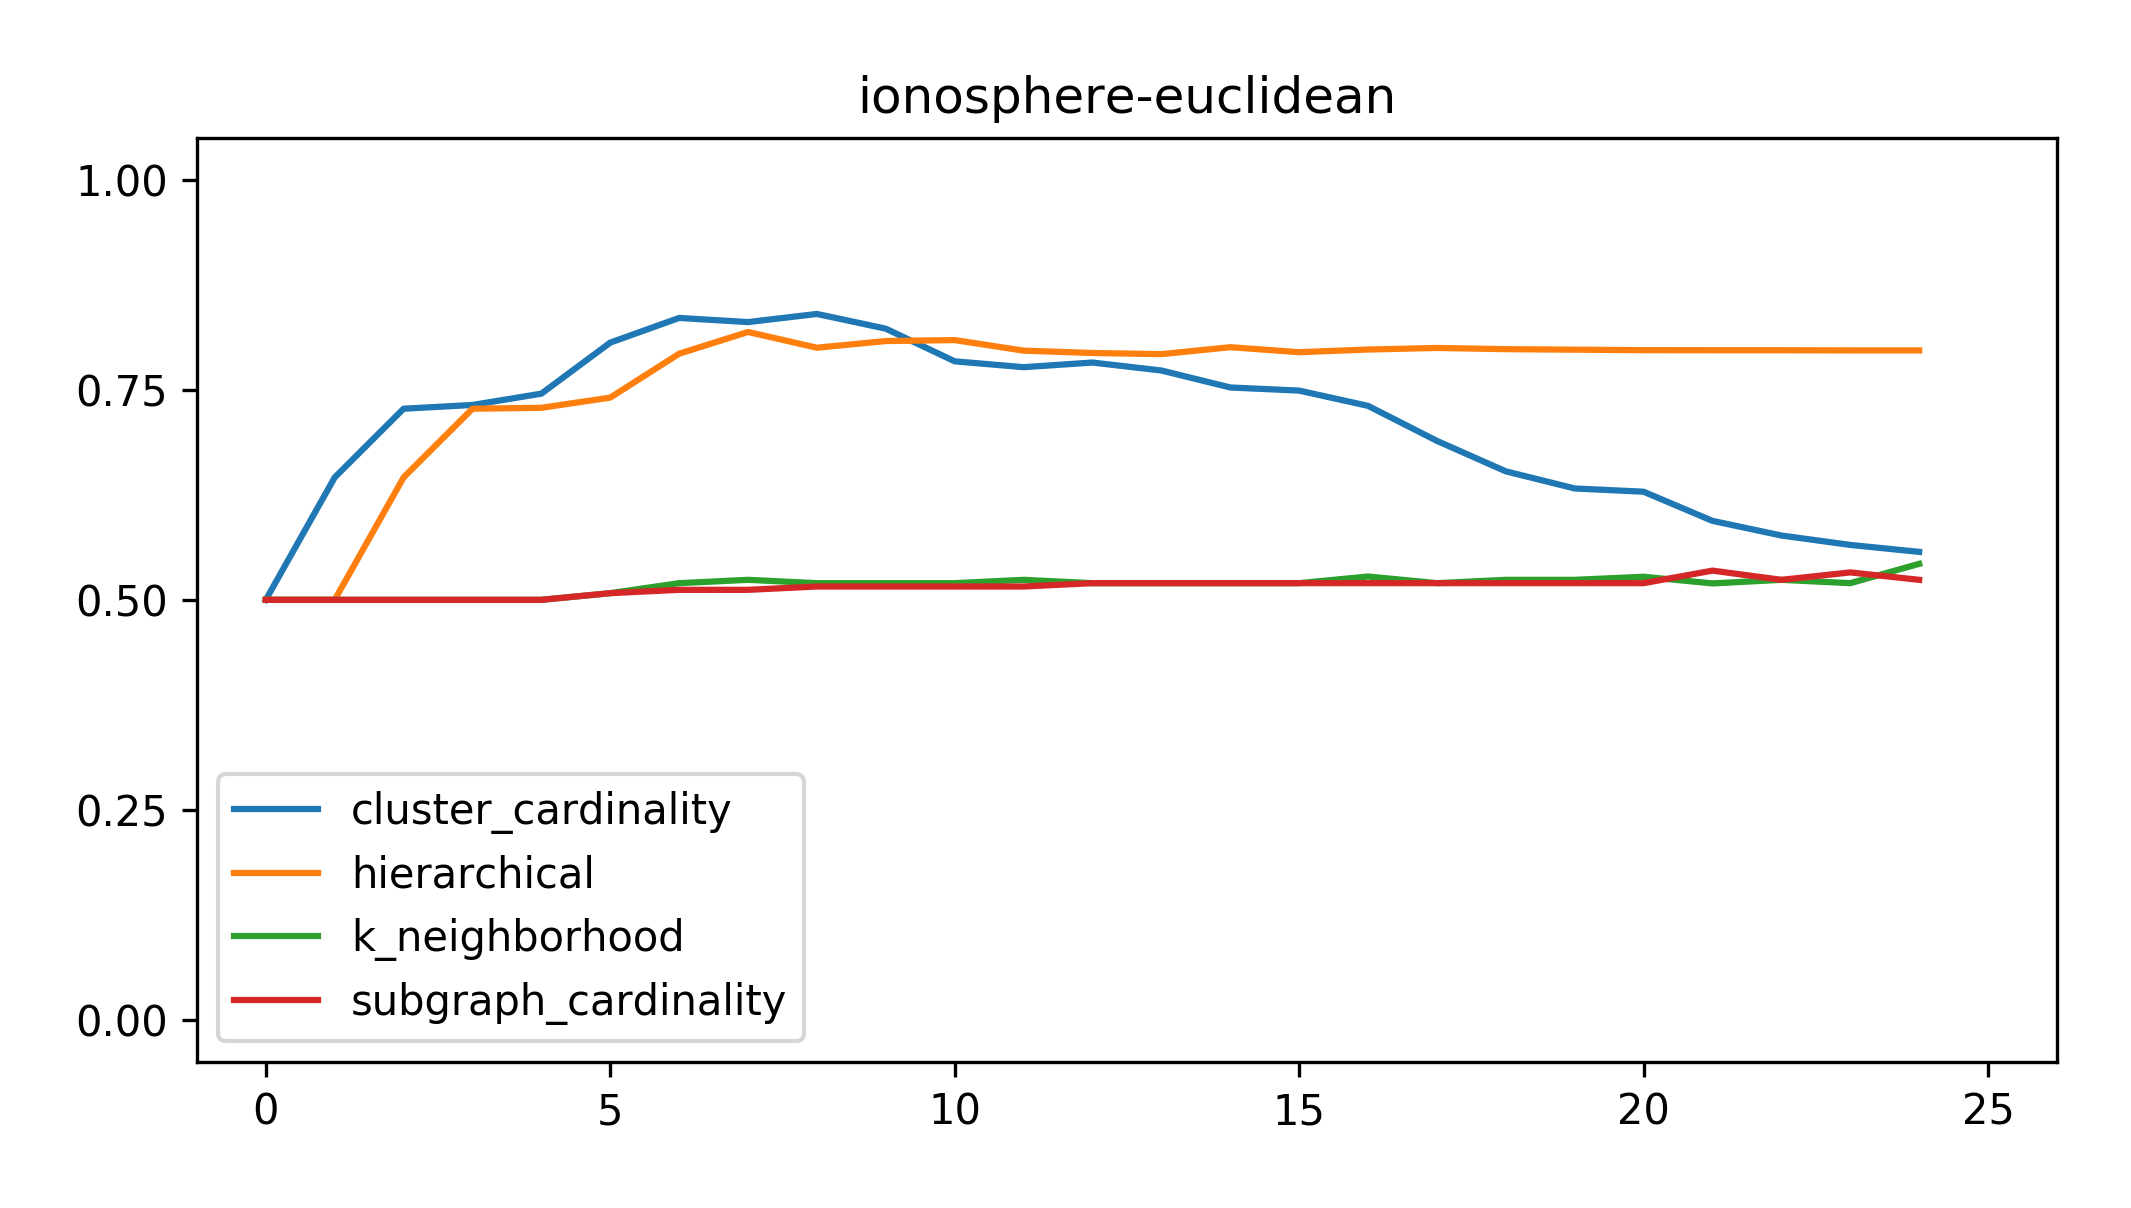
\includegraphics[width=2.2in]{kdd/static/auc_vs_depth/ionosphere-euclidean.png}
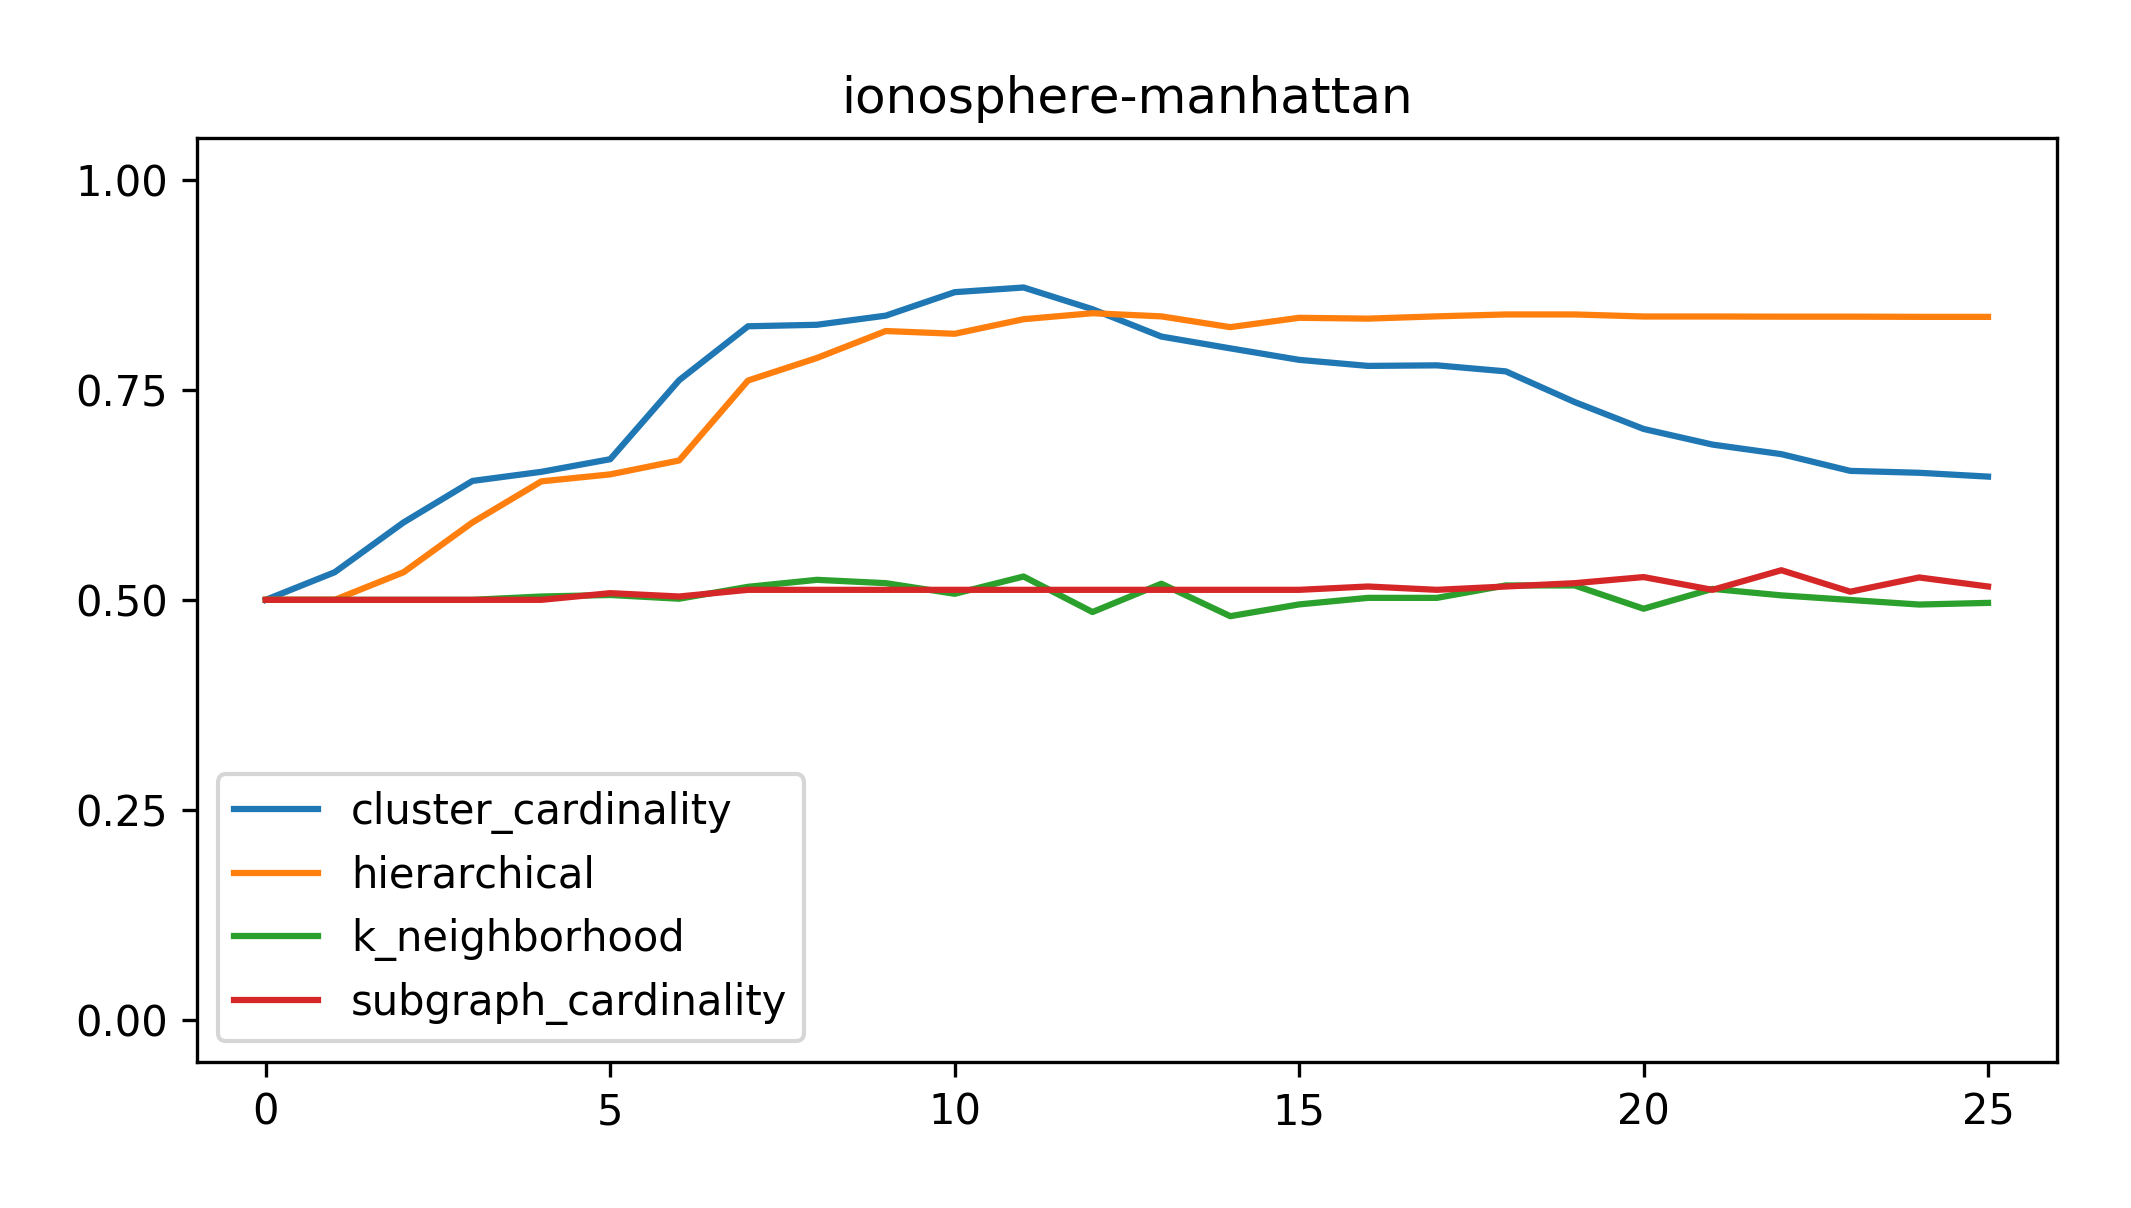
\includegraphics[width=2.2in]{kdd/static/auc_vs_depth/ionosphere-manhattan.png}

\caption{
Plots of ROC-AUC vs Depth for our mearures of Anomolousness.
}

\label{results:datasets_1}
\end{figure*}

\begin{figure*}[!t]
\centering
% Lympho
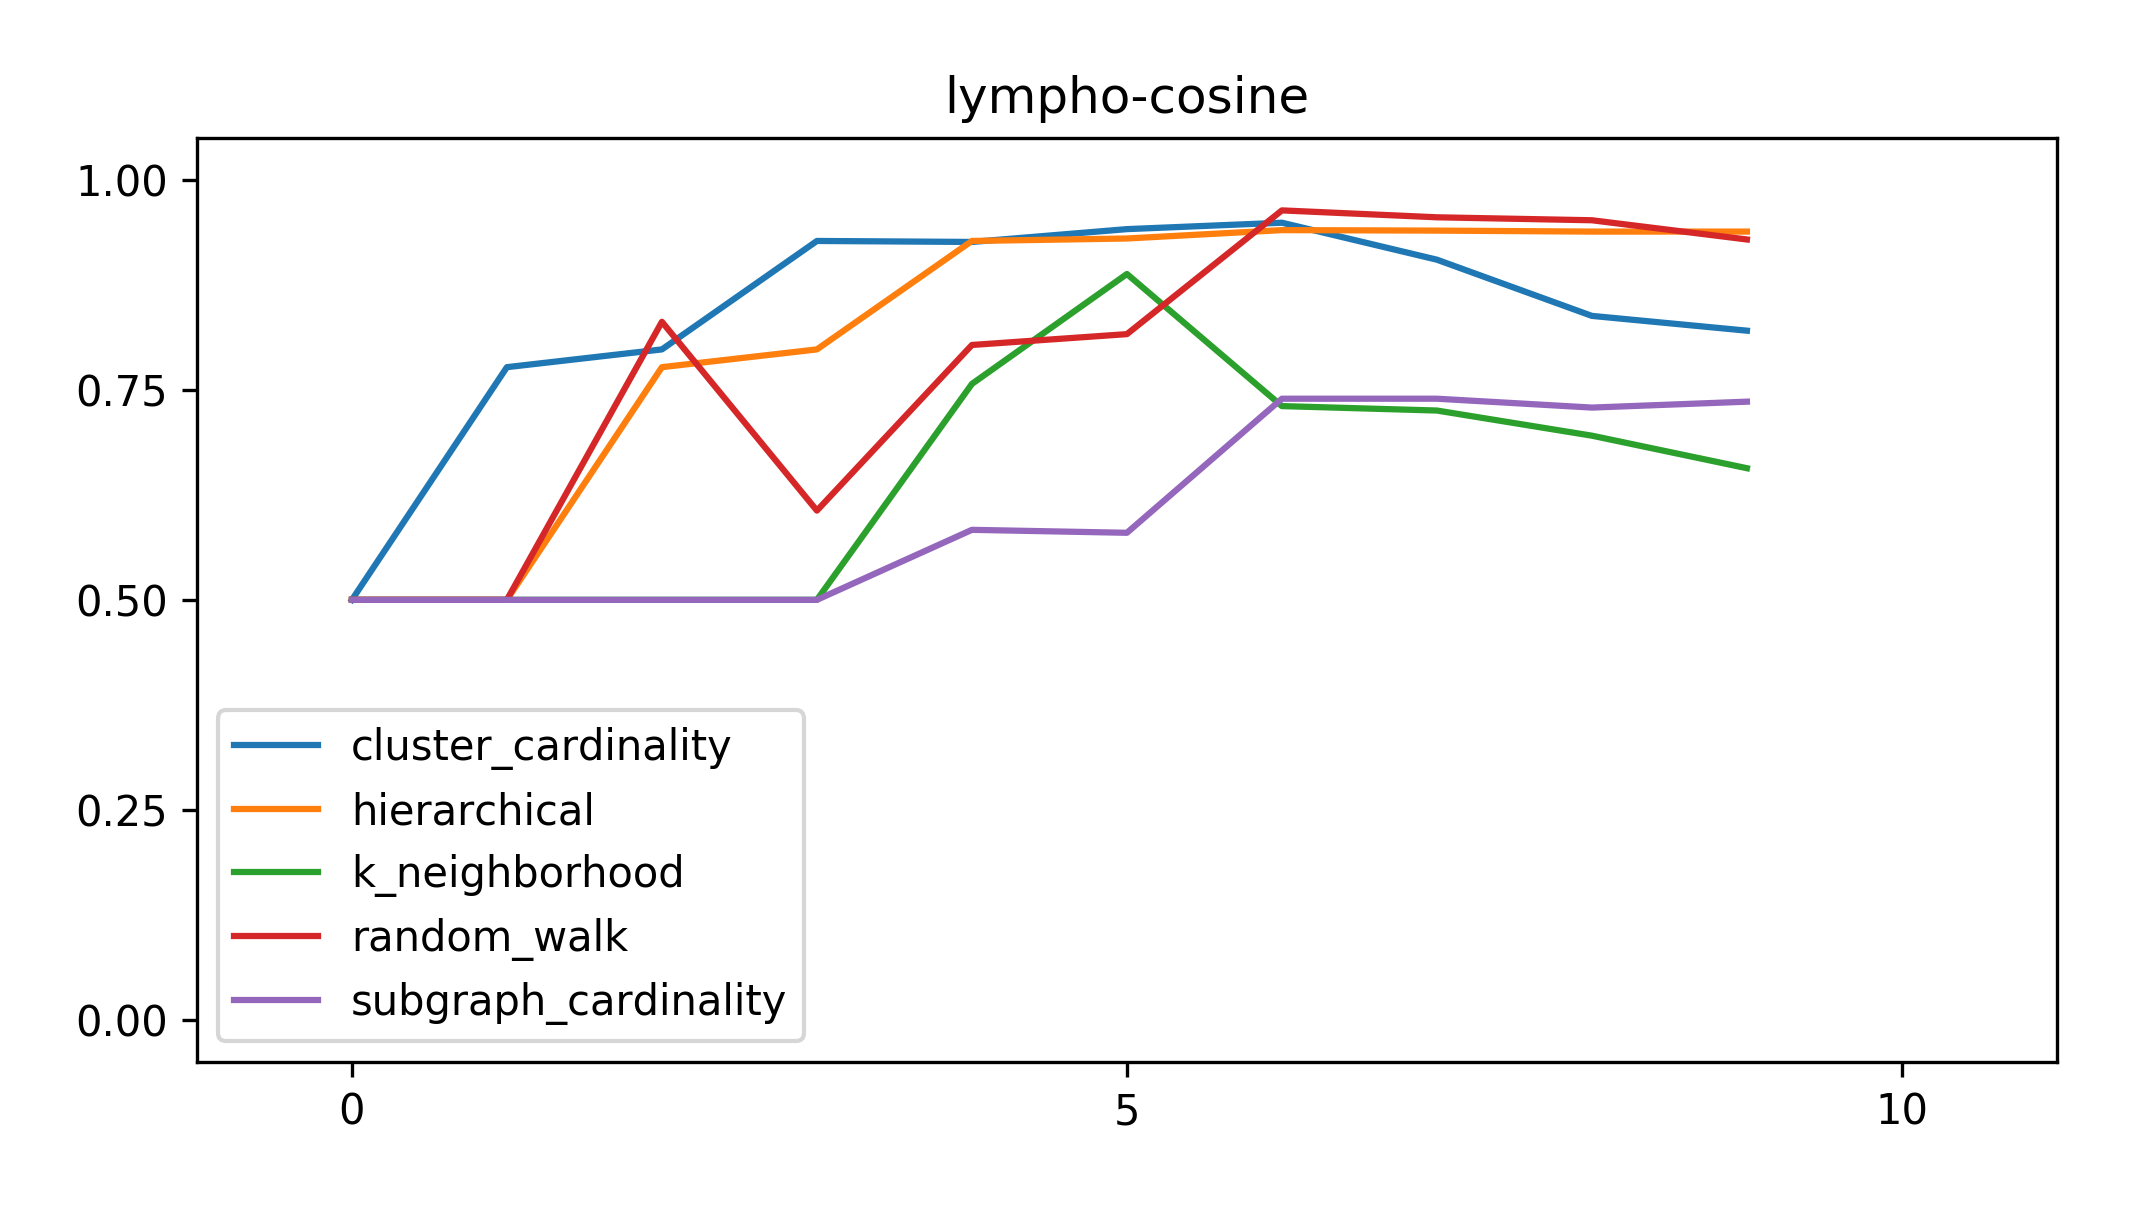
\includegraphics[width=2.2in]{kdd/static/auc_vs_depth/lympho-cosine.png}
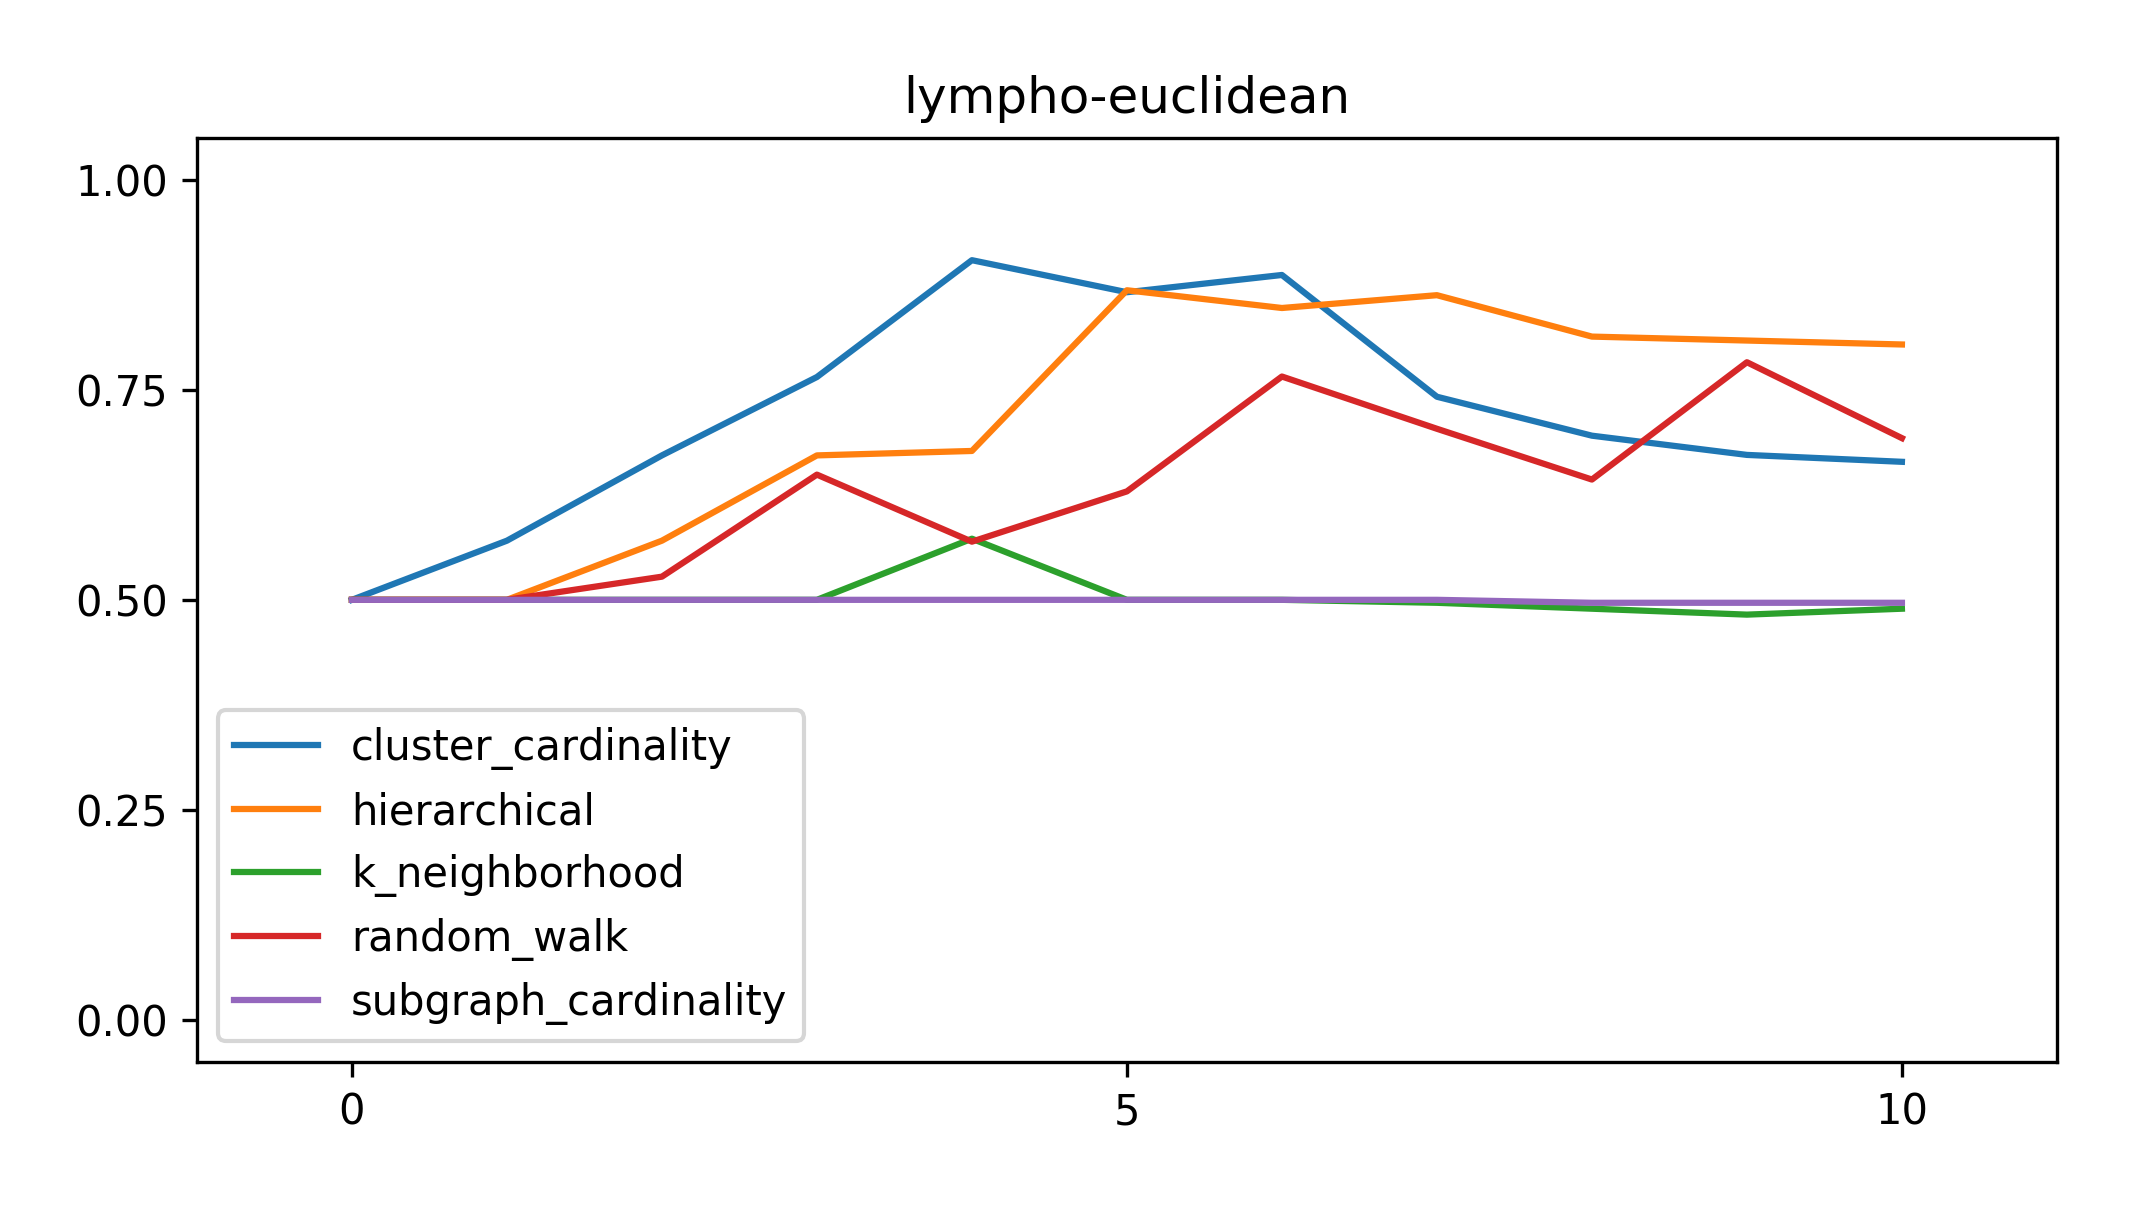
\includegraphics[width=2.2in]{kdd/static/auc_vs_depth/lympho-euclidean.png}
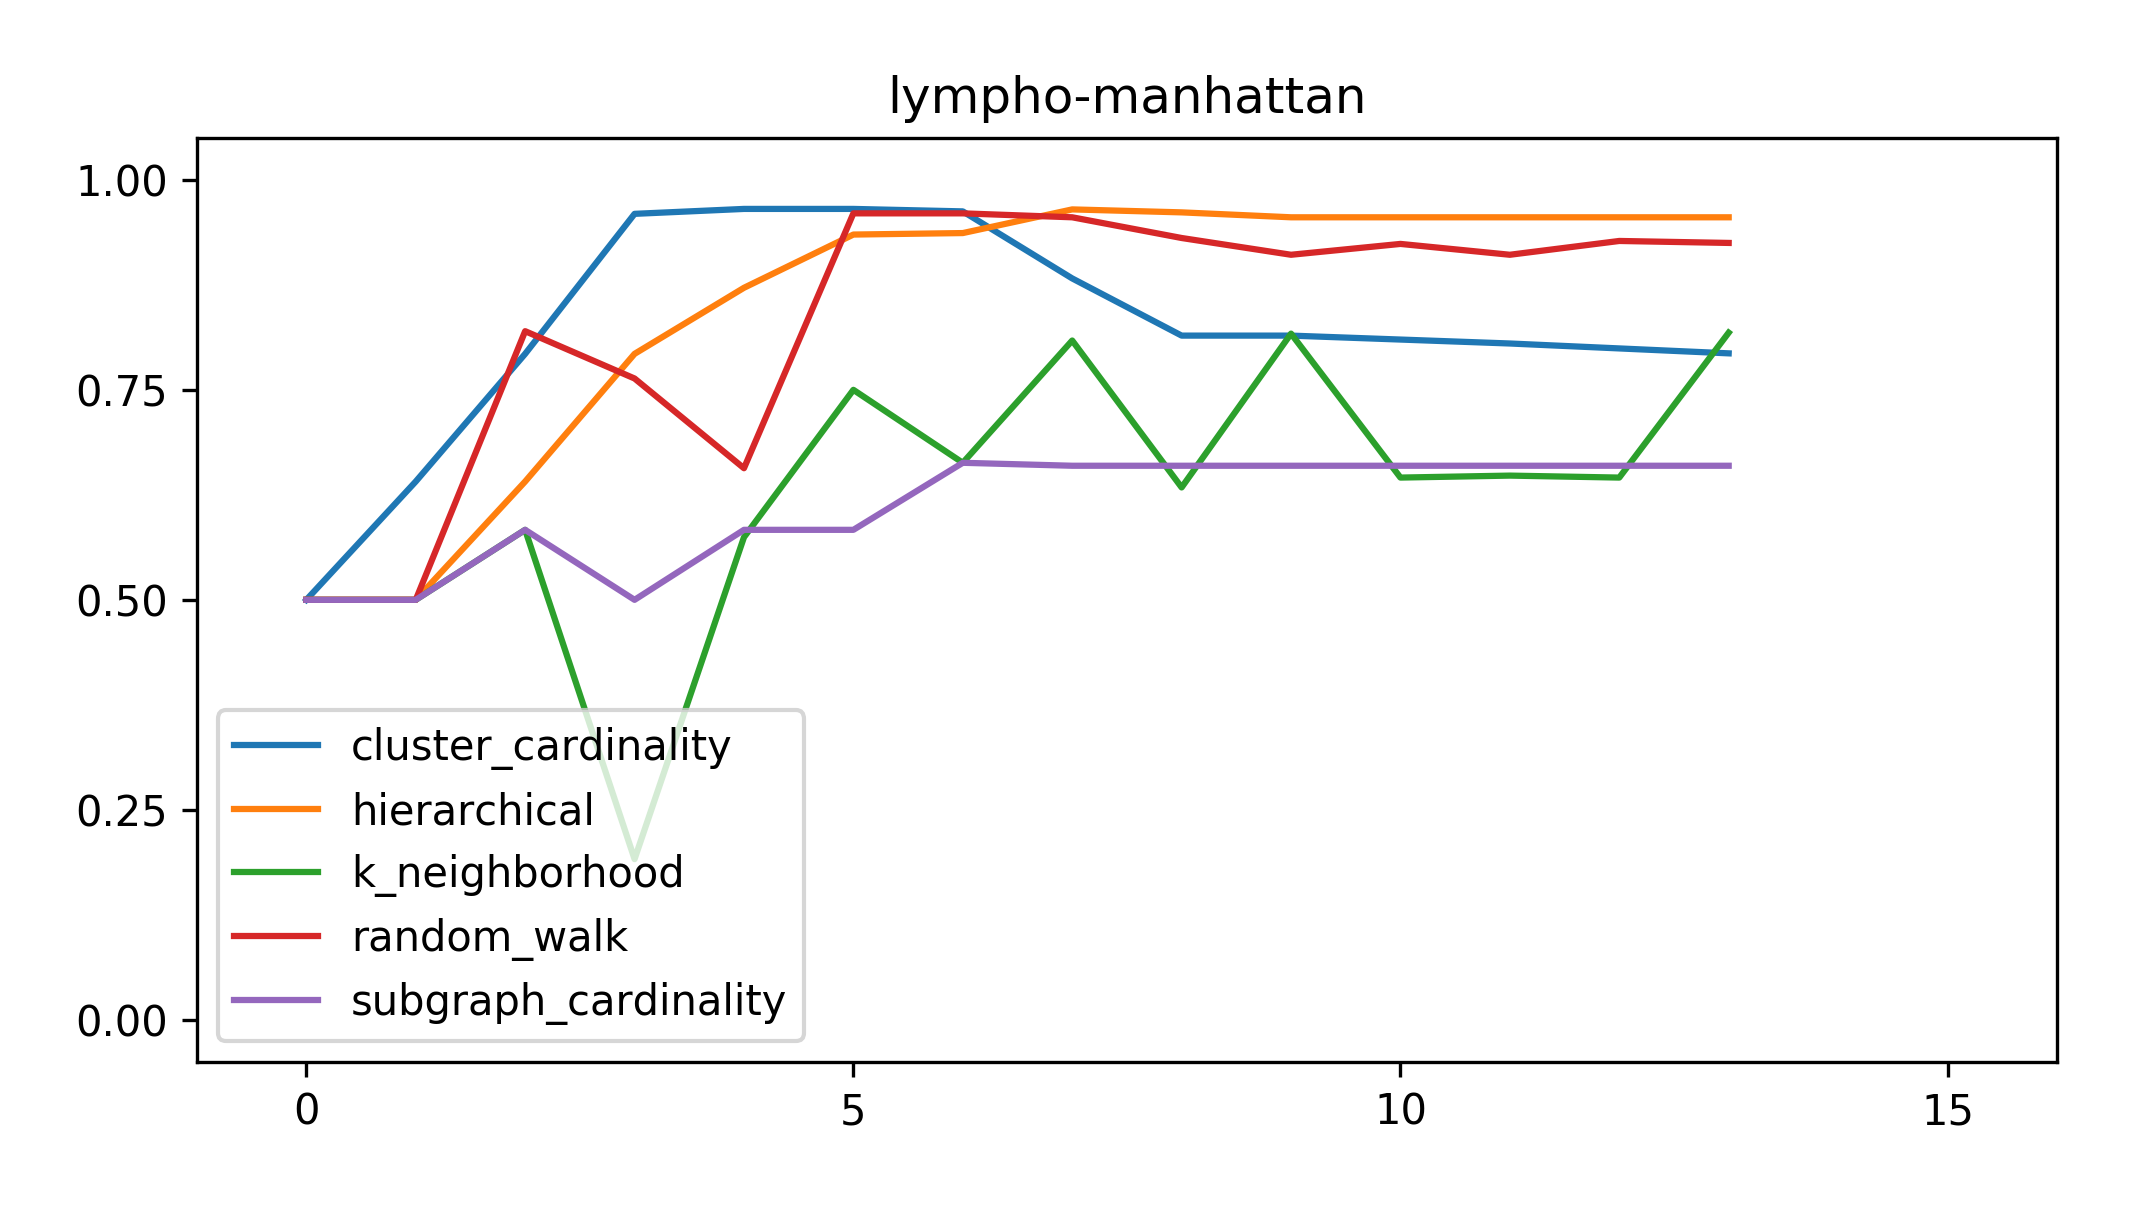
\includegraphics[width=2.2in]{kdd/static/auc_vs_depth/lympho-manhattan.png}

% Mnist
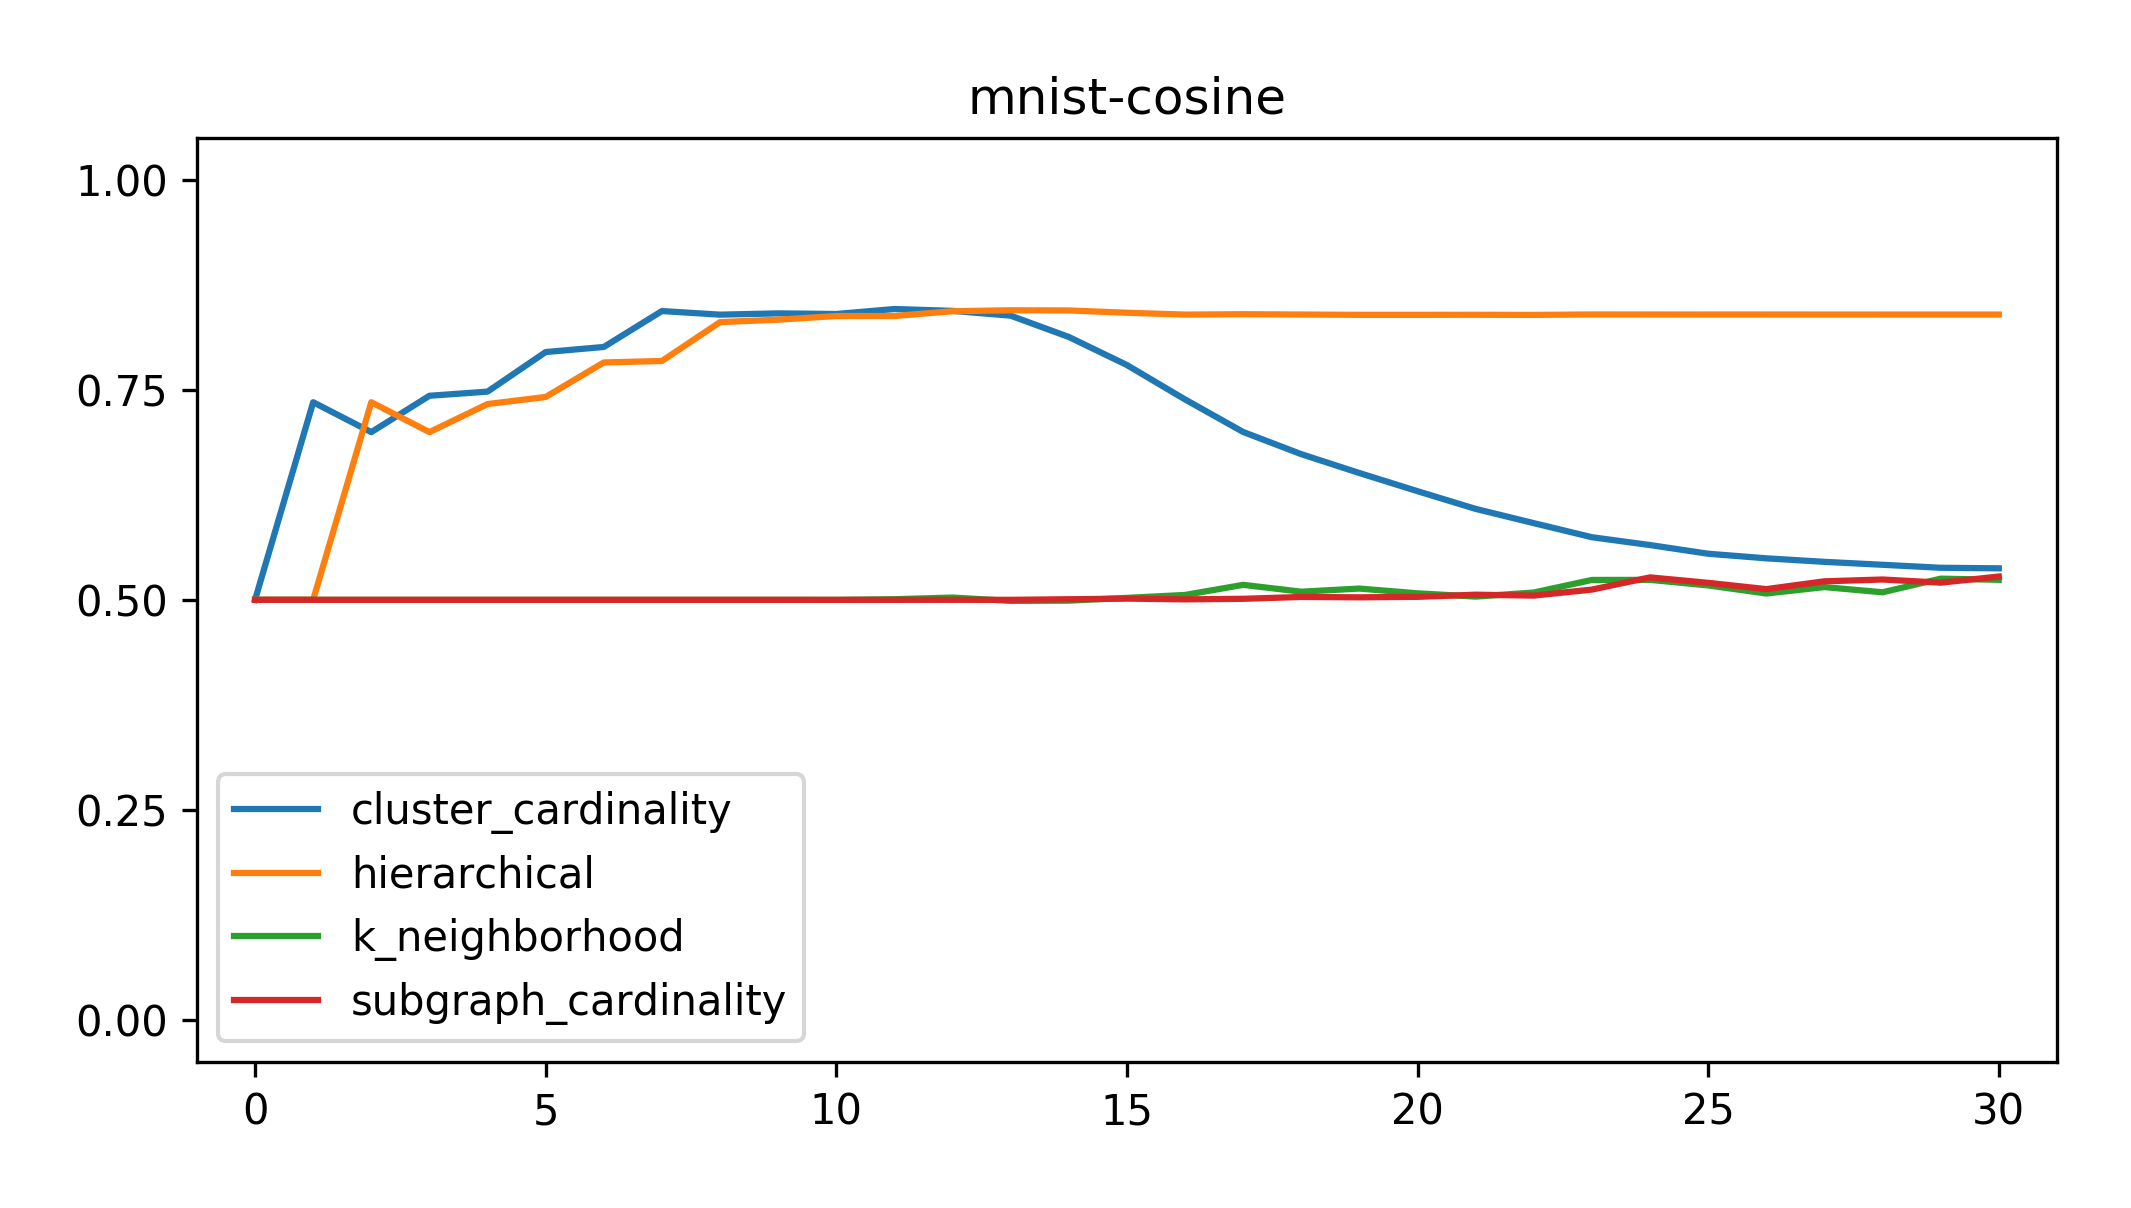
\includegraphics[width=2.2in]{kdd/static/auc_vs_depth/mnist-cosine.png}
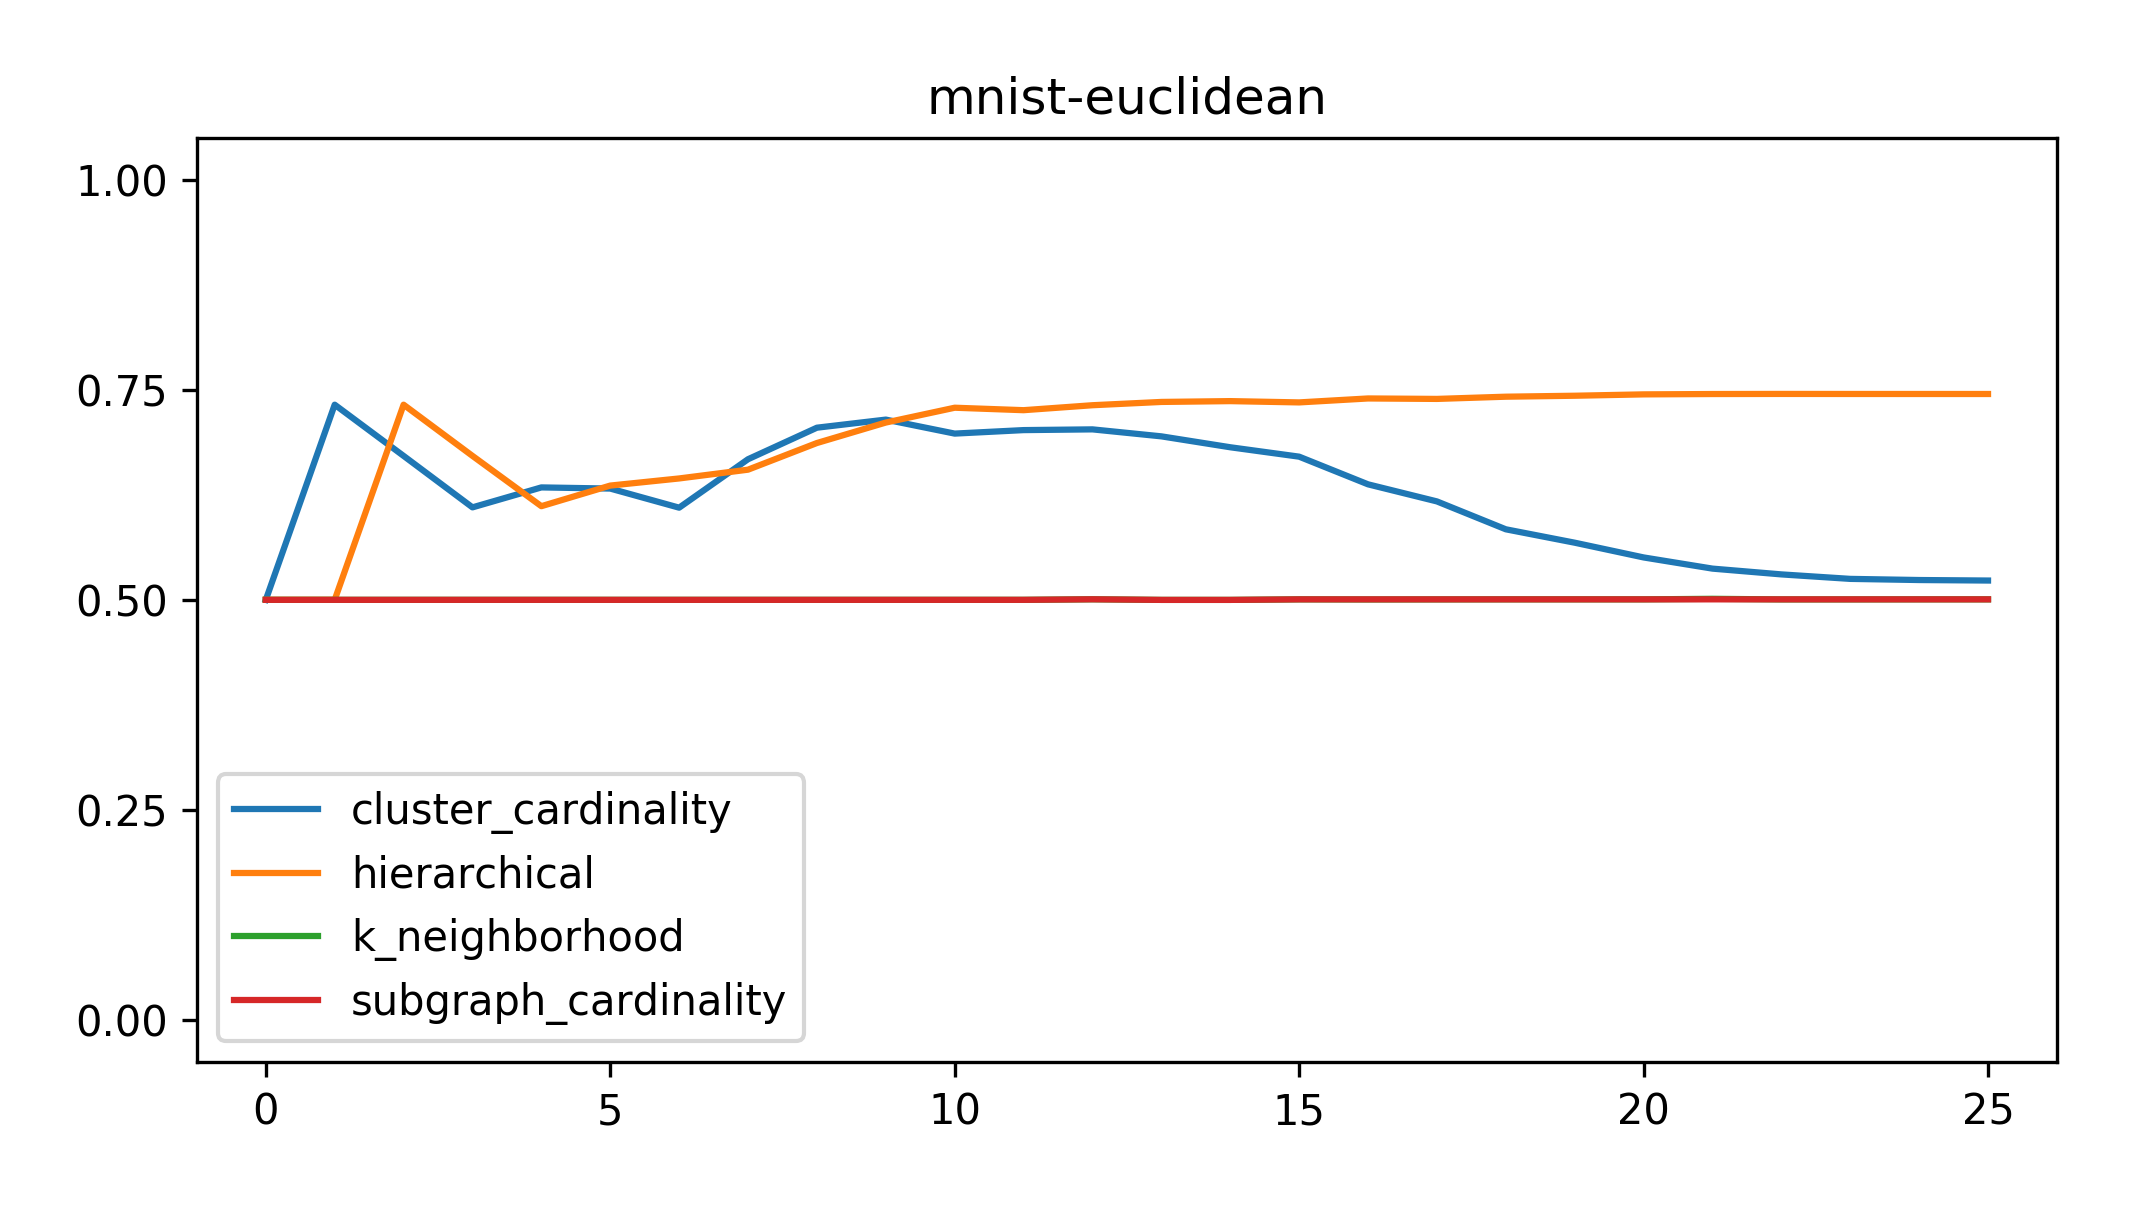
\includegraphics[width=2.2in]{kdd/static/auc_vs_depth/mnist-euclidean.png}
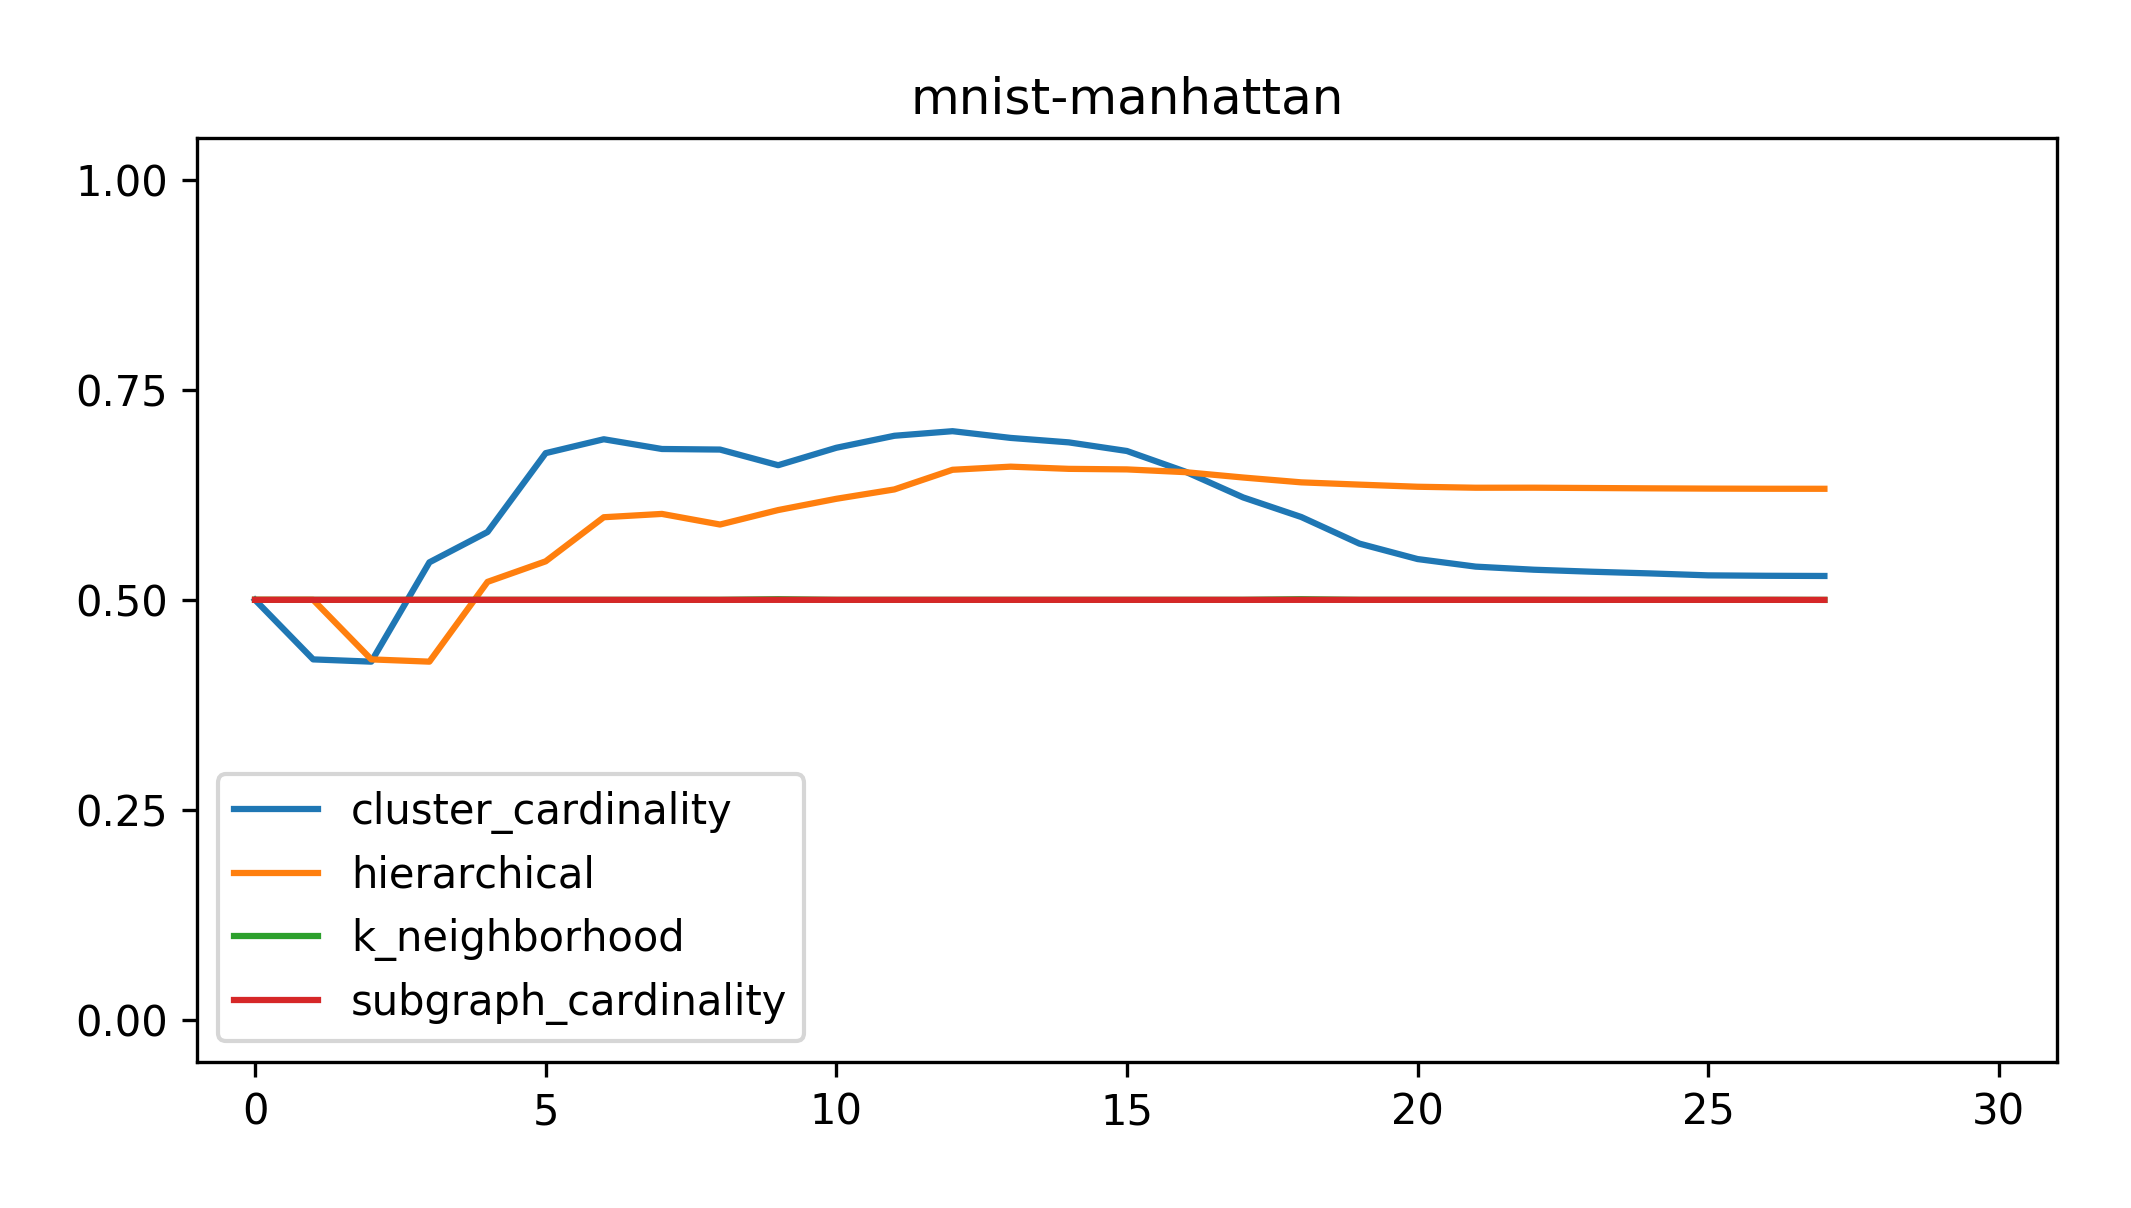
\includegraphics[width=2.2in]{kdd/static/auc_vs_depth/mnist-manhattan.png}

% Musk
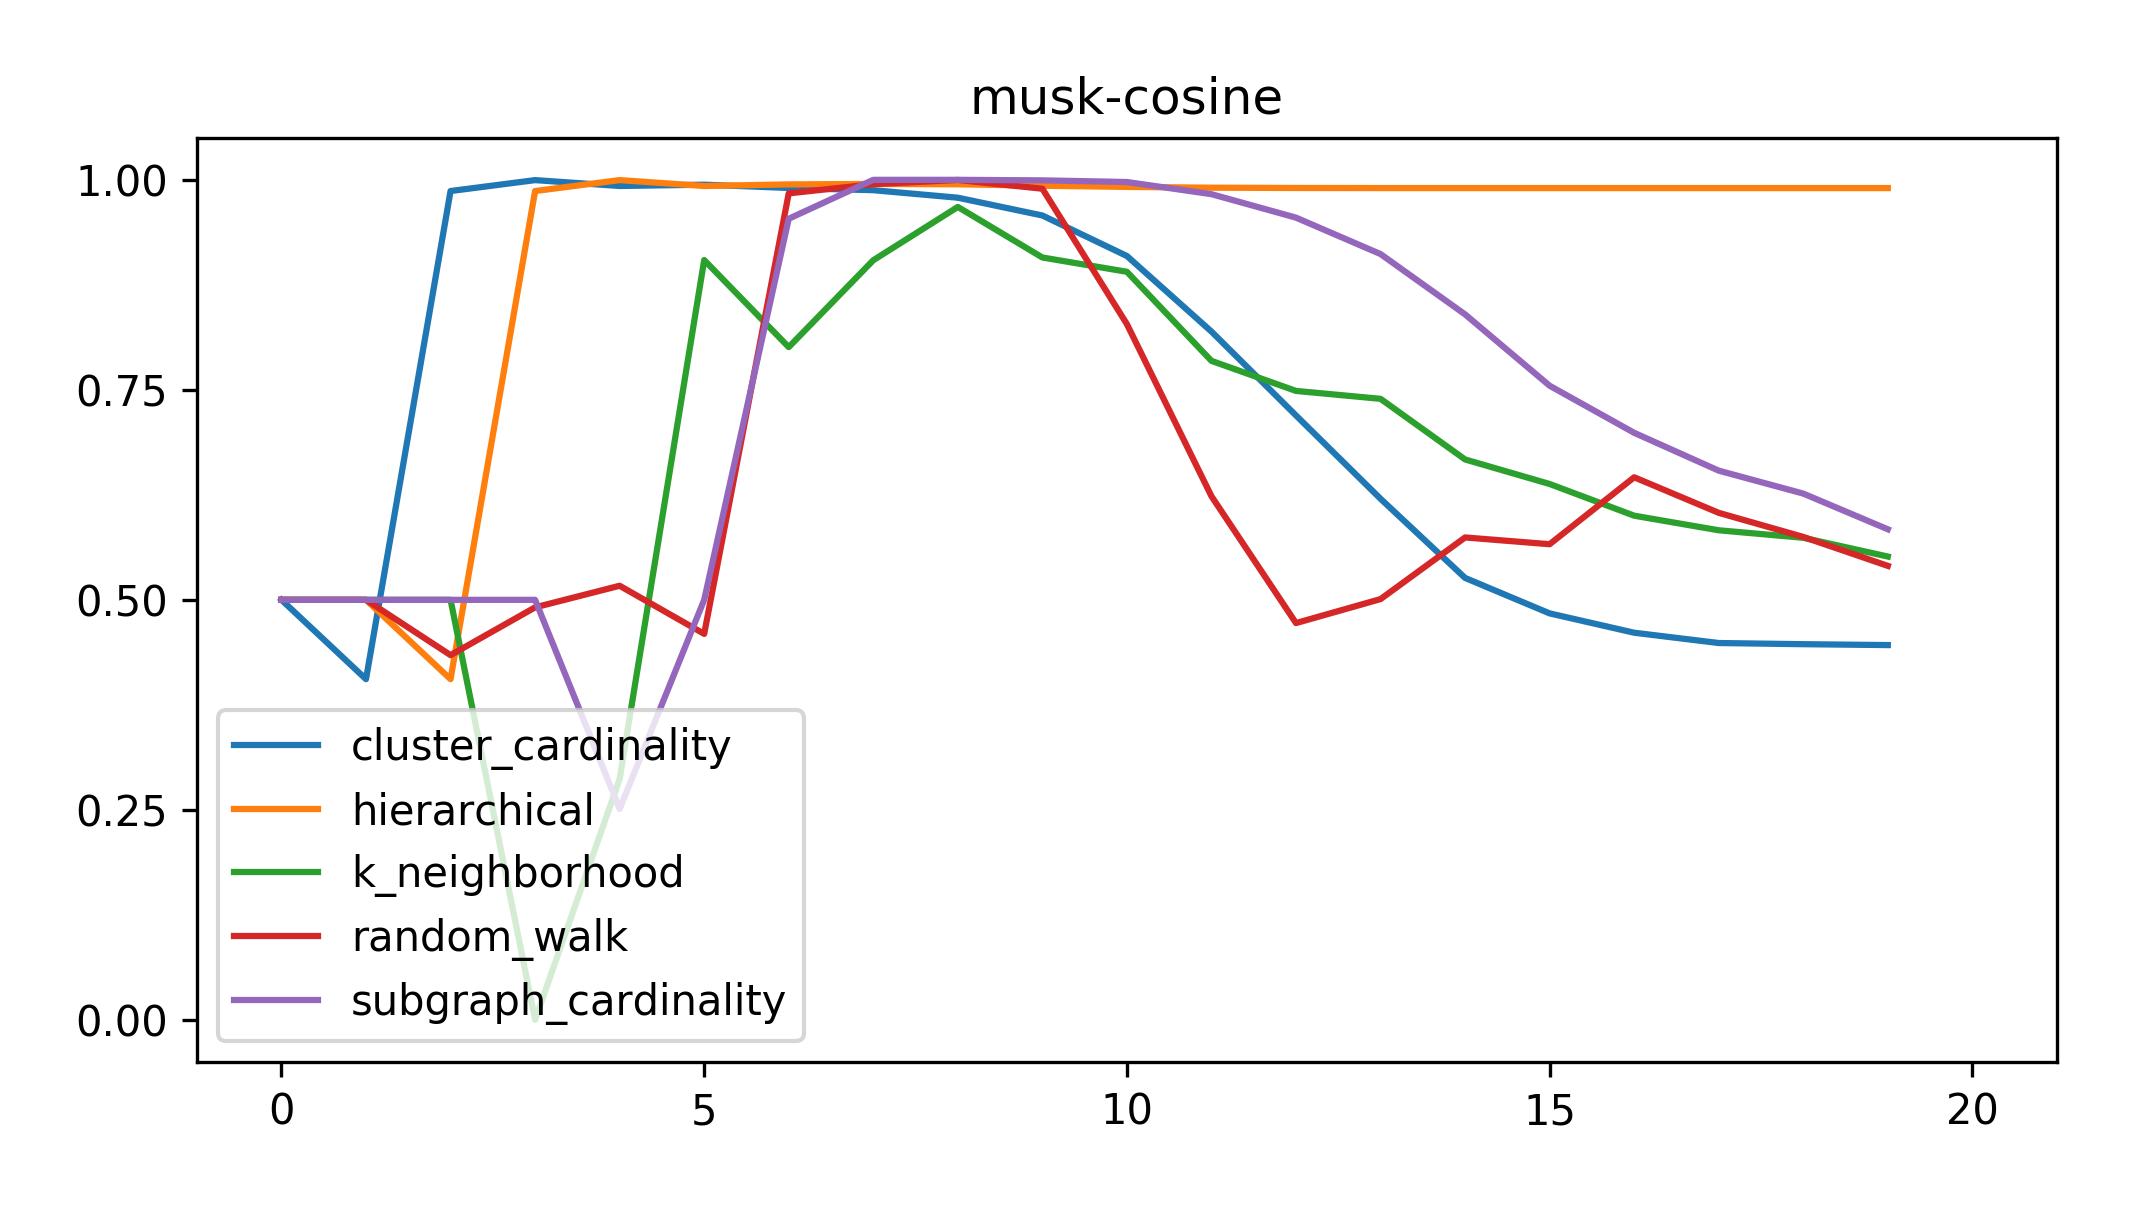
\includegraphics[width=2.2in]{kdd/static/auc_vs_depth/musk-cosine.png}
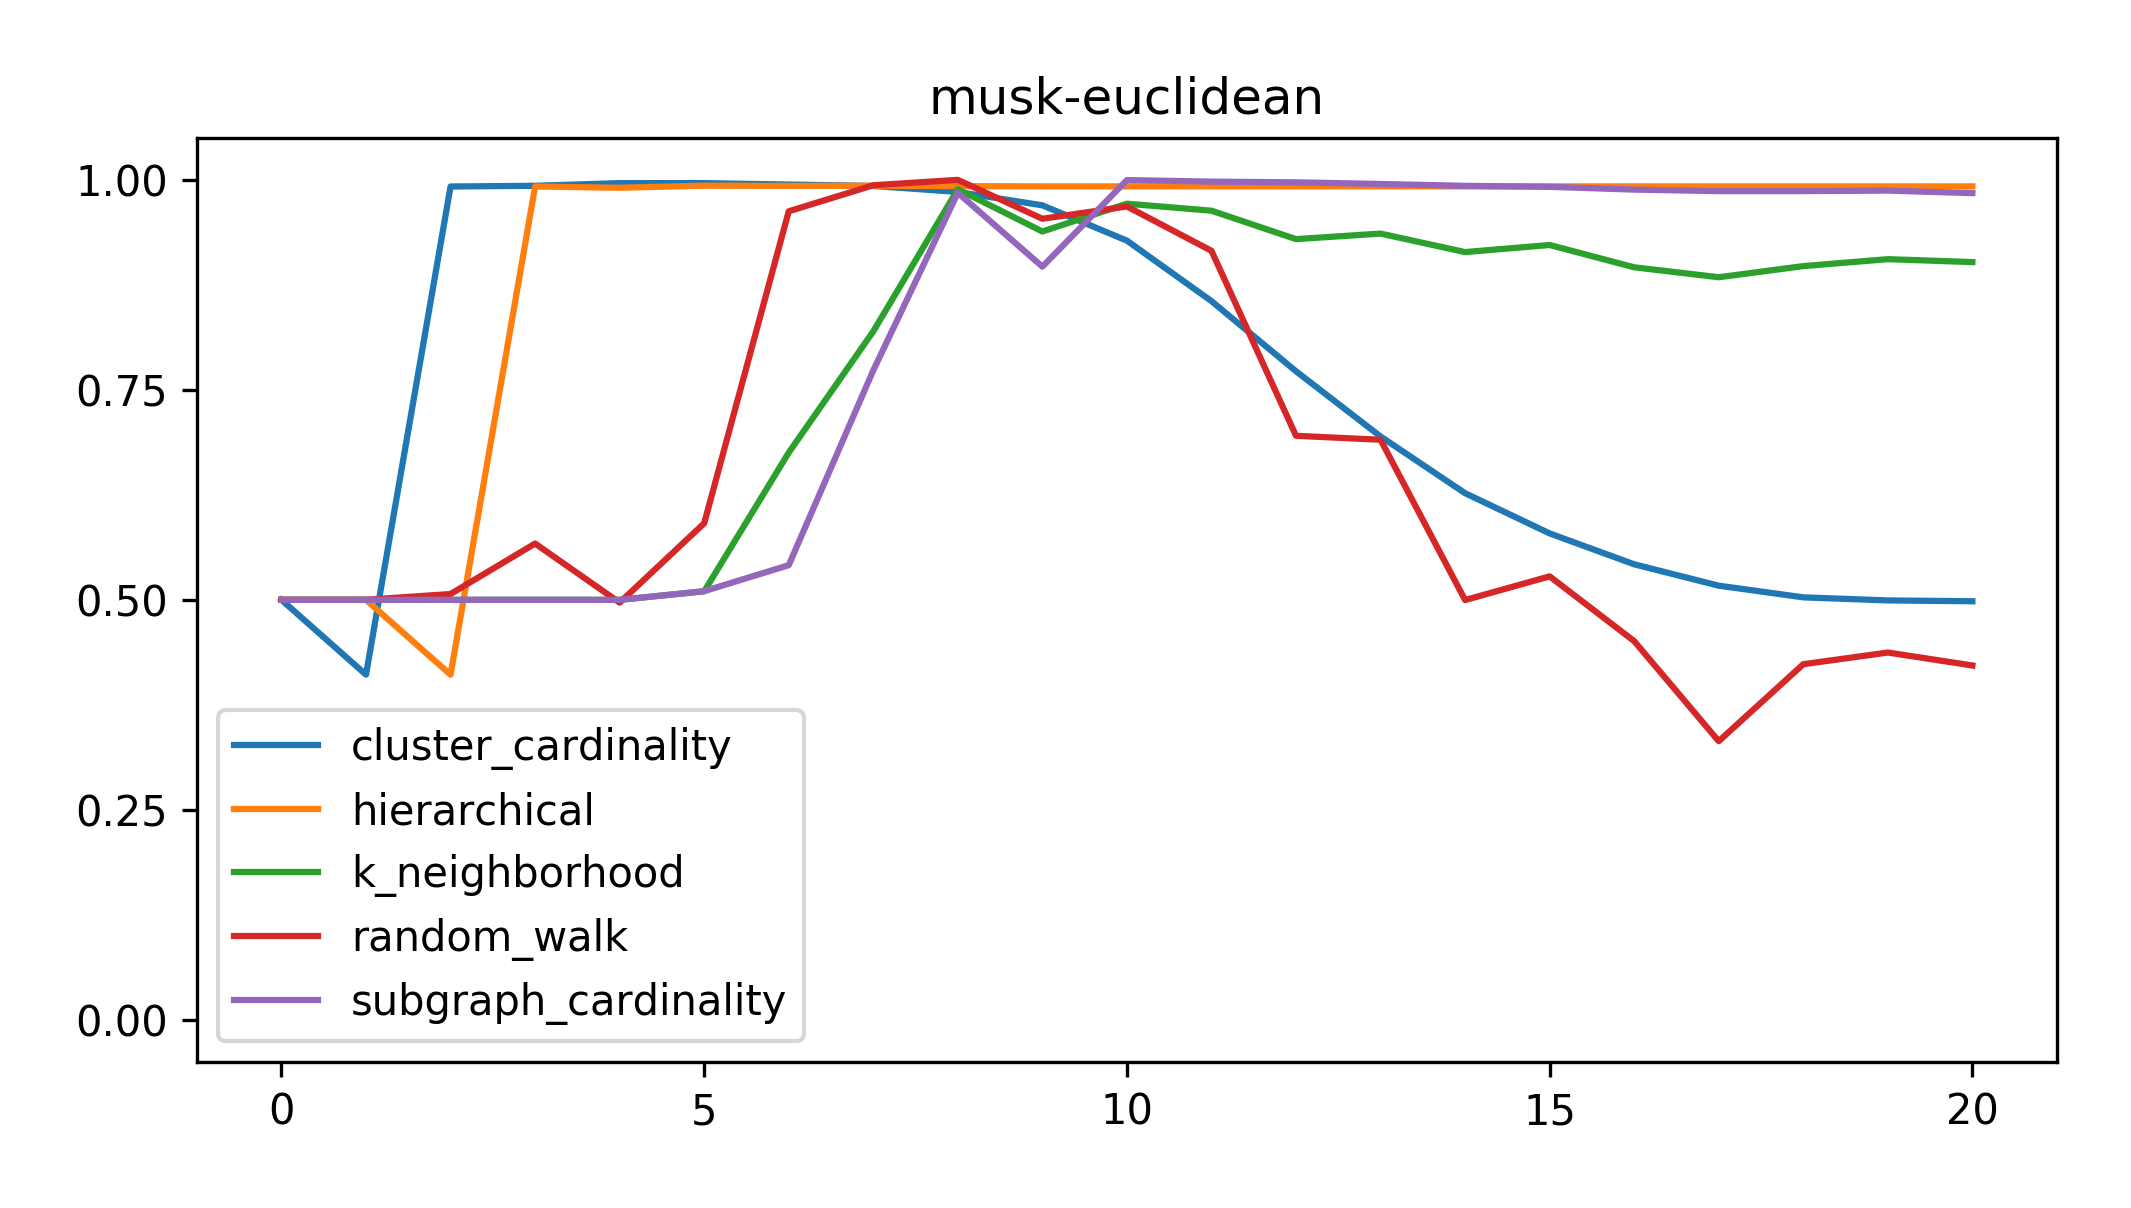
\includegraphics[width=2.2in]{kdd/static/auc_vs_depth/musk-euclidean.png}
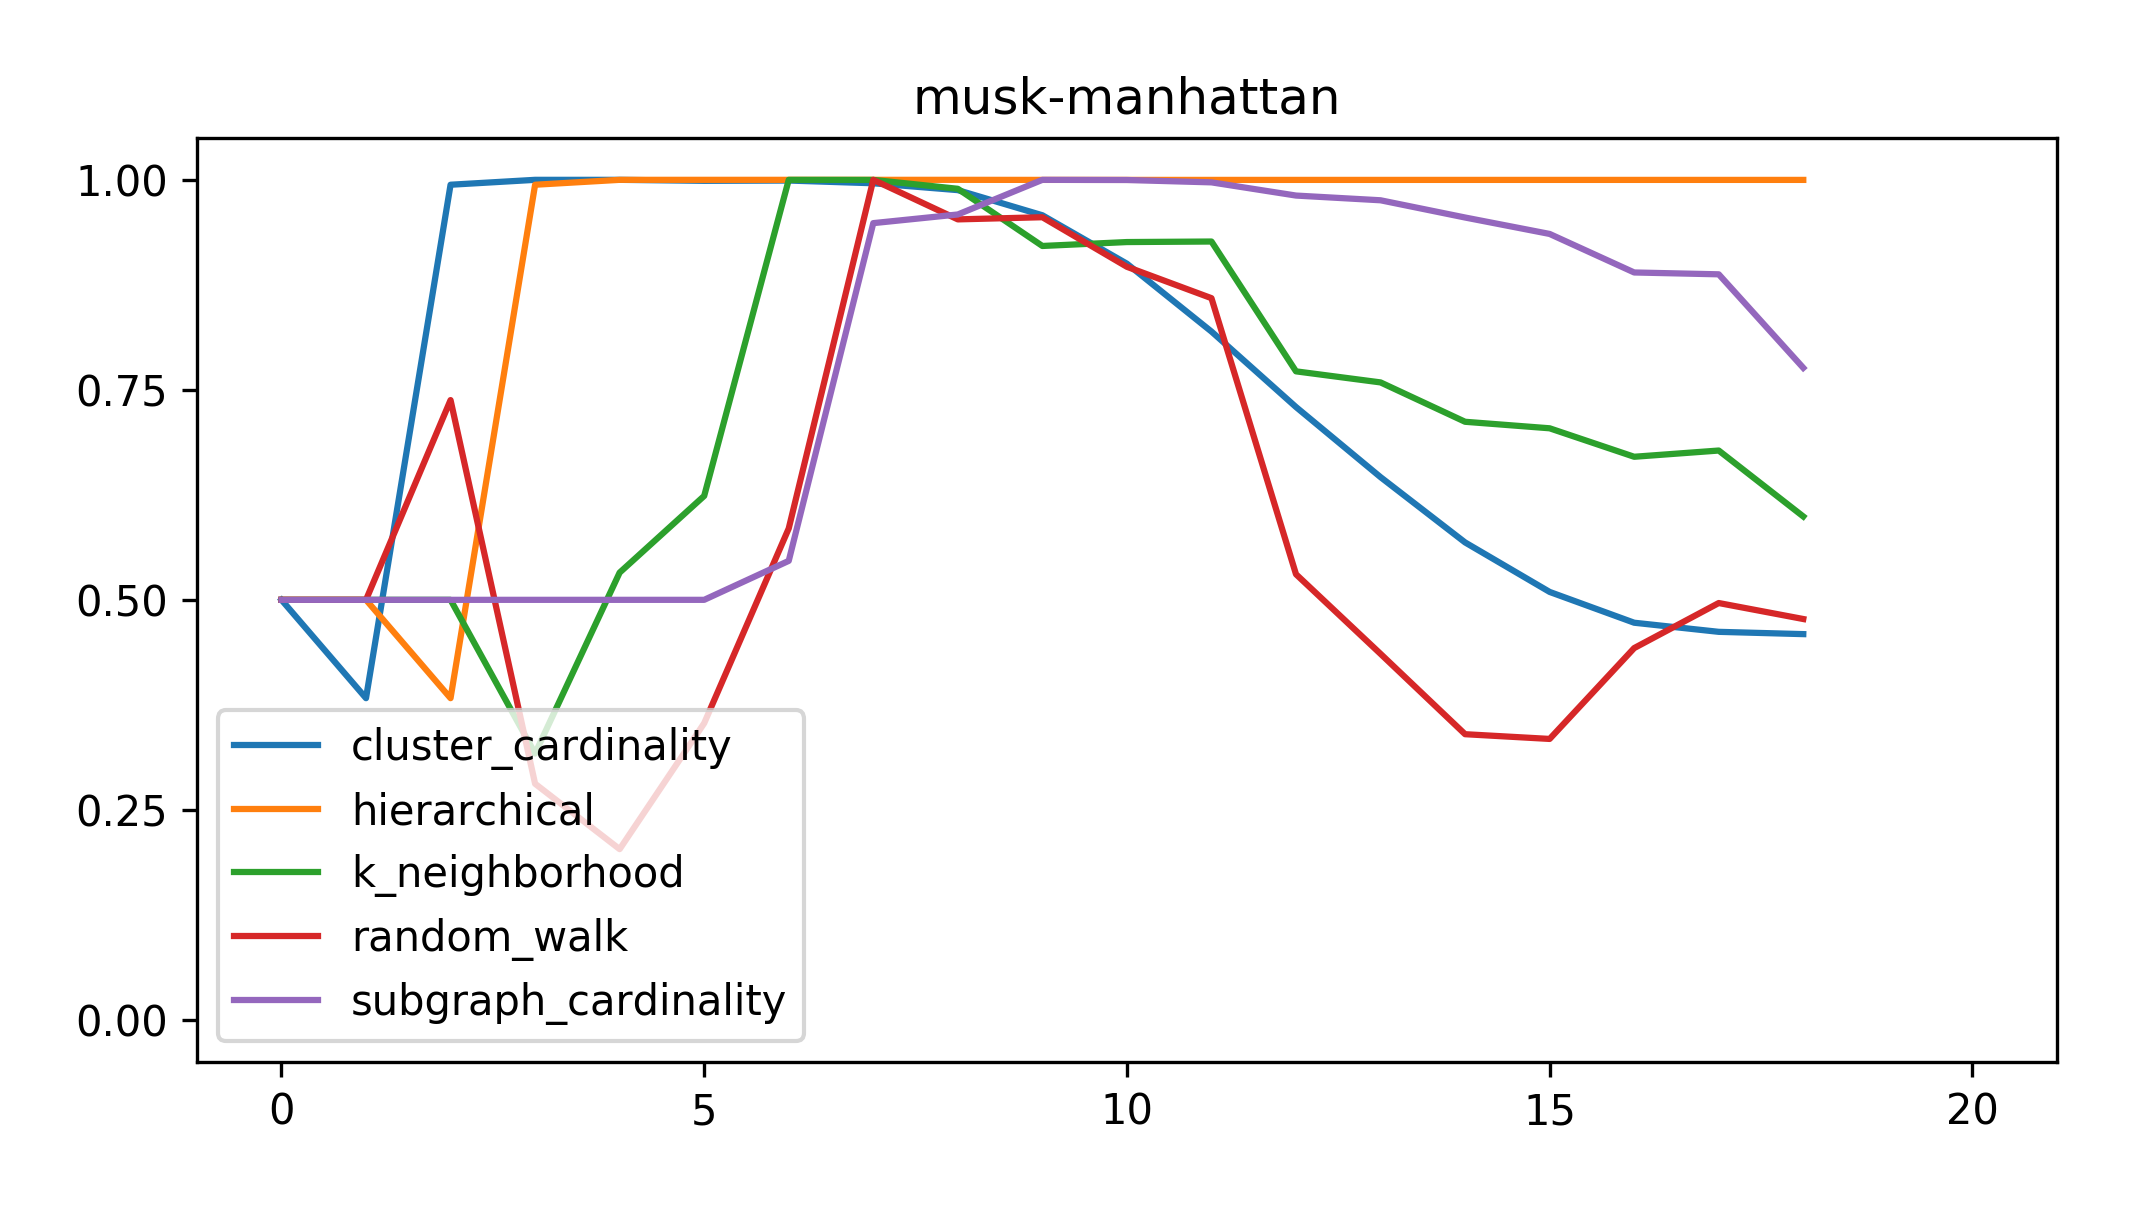
\includegraphics[width=2.2in]{kdd/static/auc_vs_depth/musk-manhattan.png}

% Optdigits
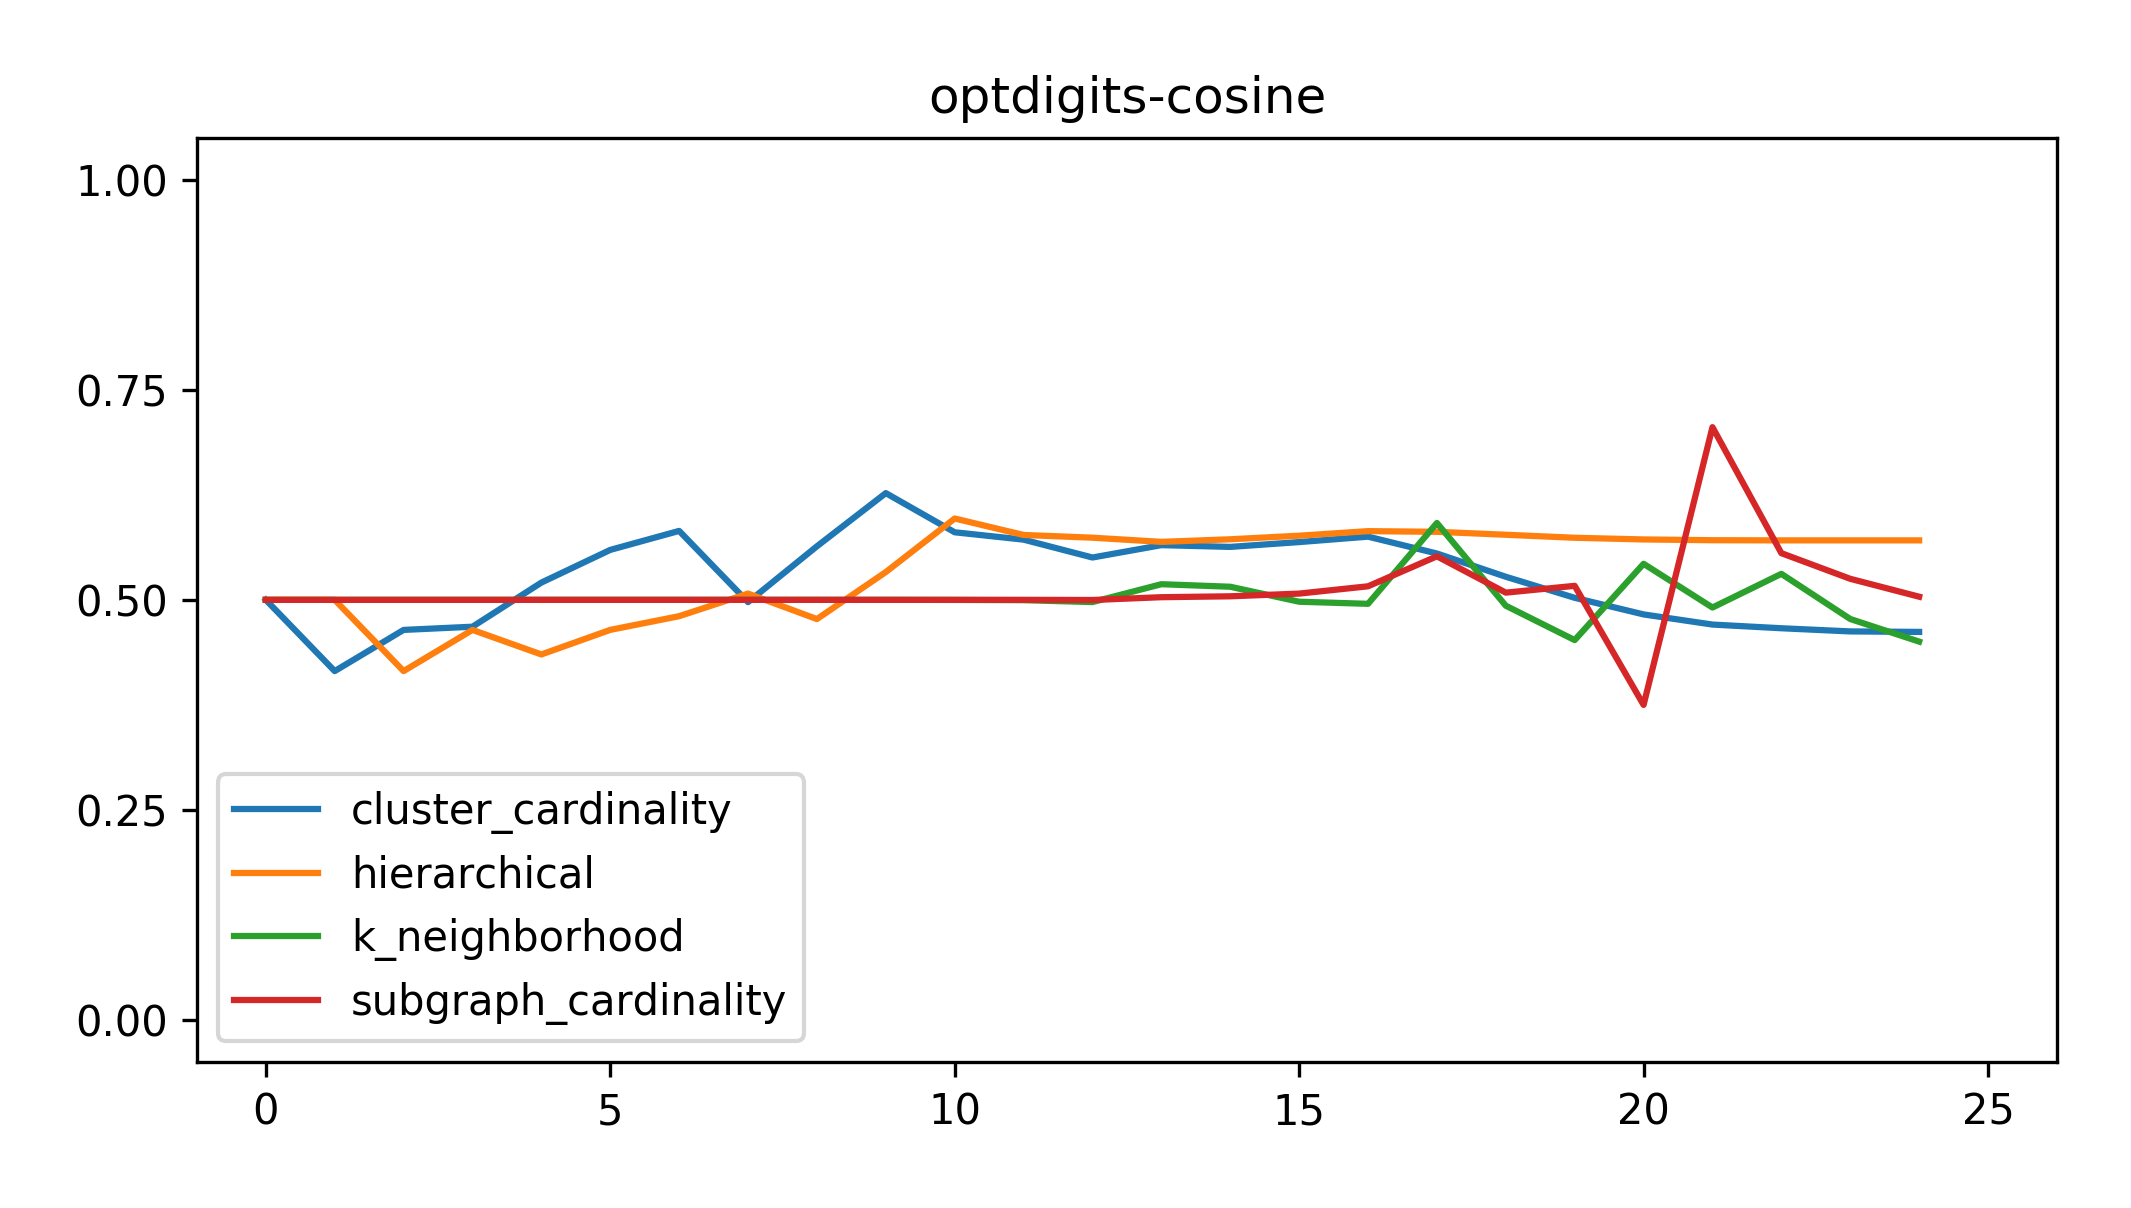
\includegraphics[width=2.2in]{kdd/static/auc_vs_depth/optdigits-cosine.png}
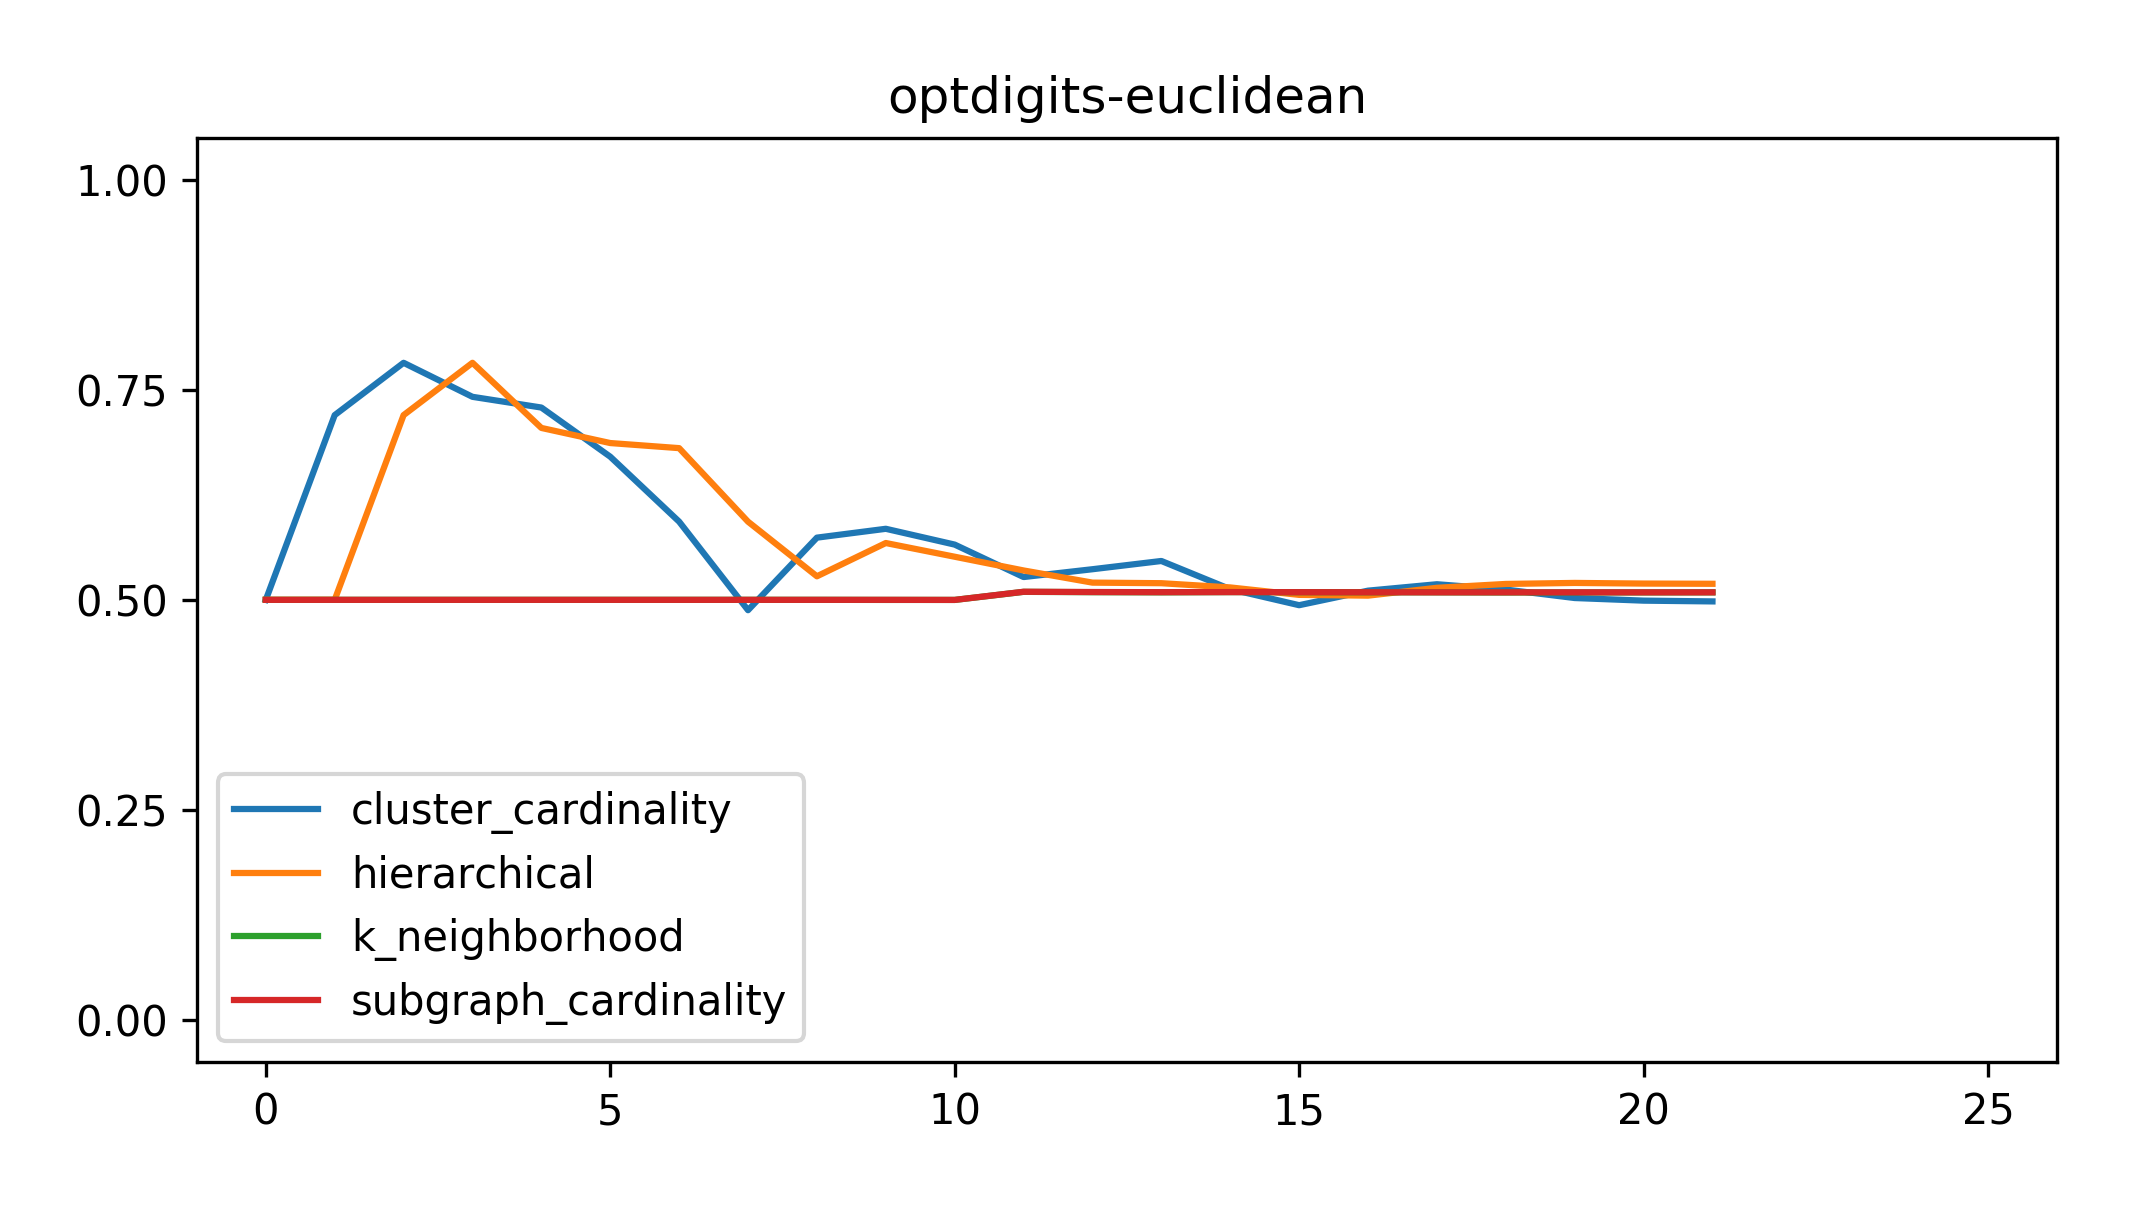
\includegraphics[width=2.2in]{kdd/static/auc_vs_depth/optdigits-euclidean.png}
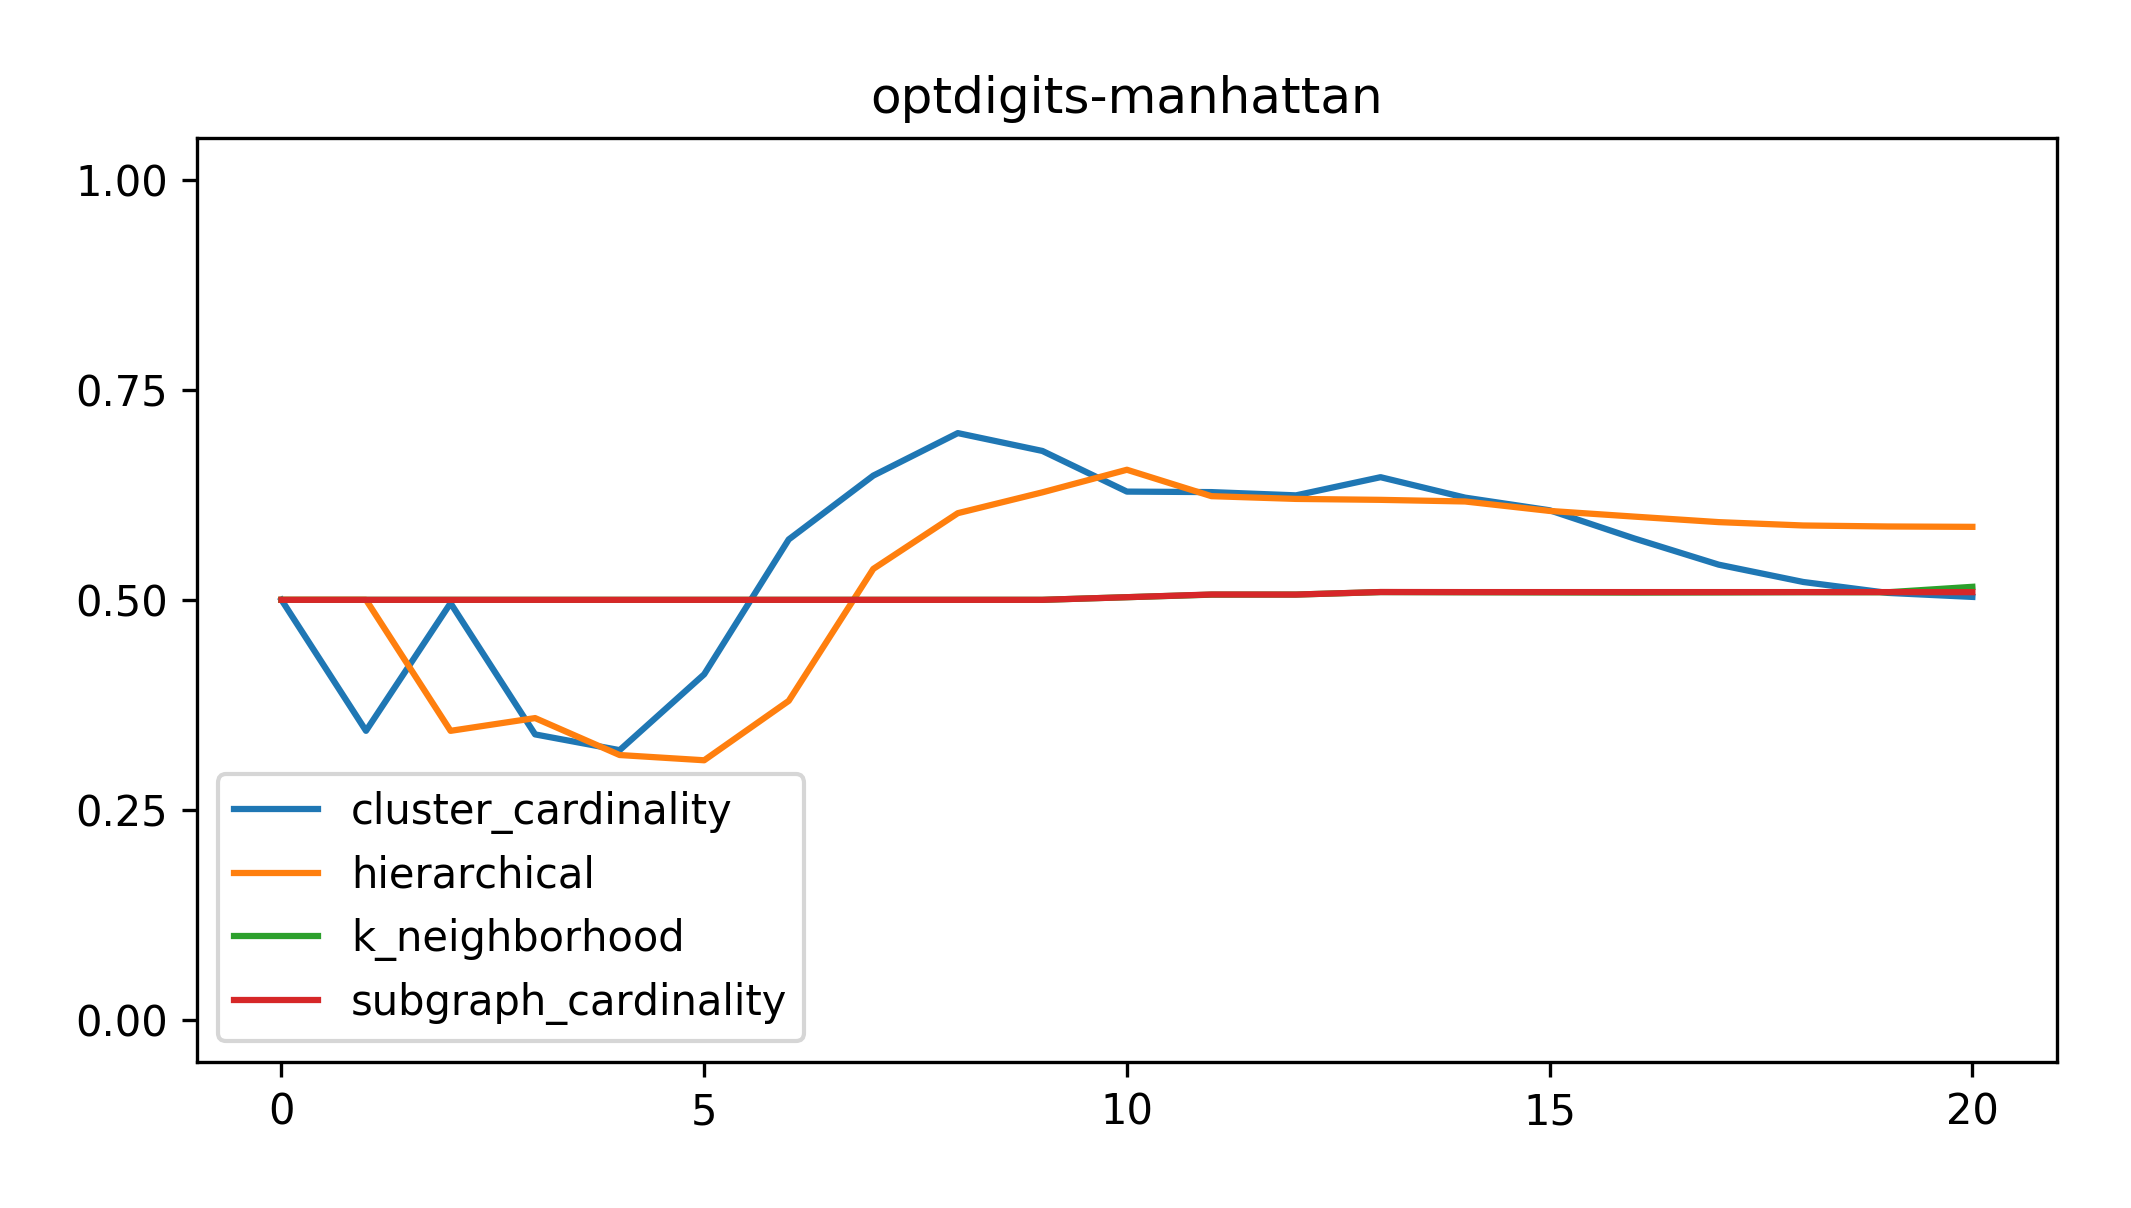
\includegraphics[width=2.2in]{kdd/static/auc_vs_depth/optdigits-manhattan.png}

% Pima
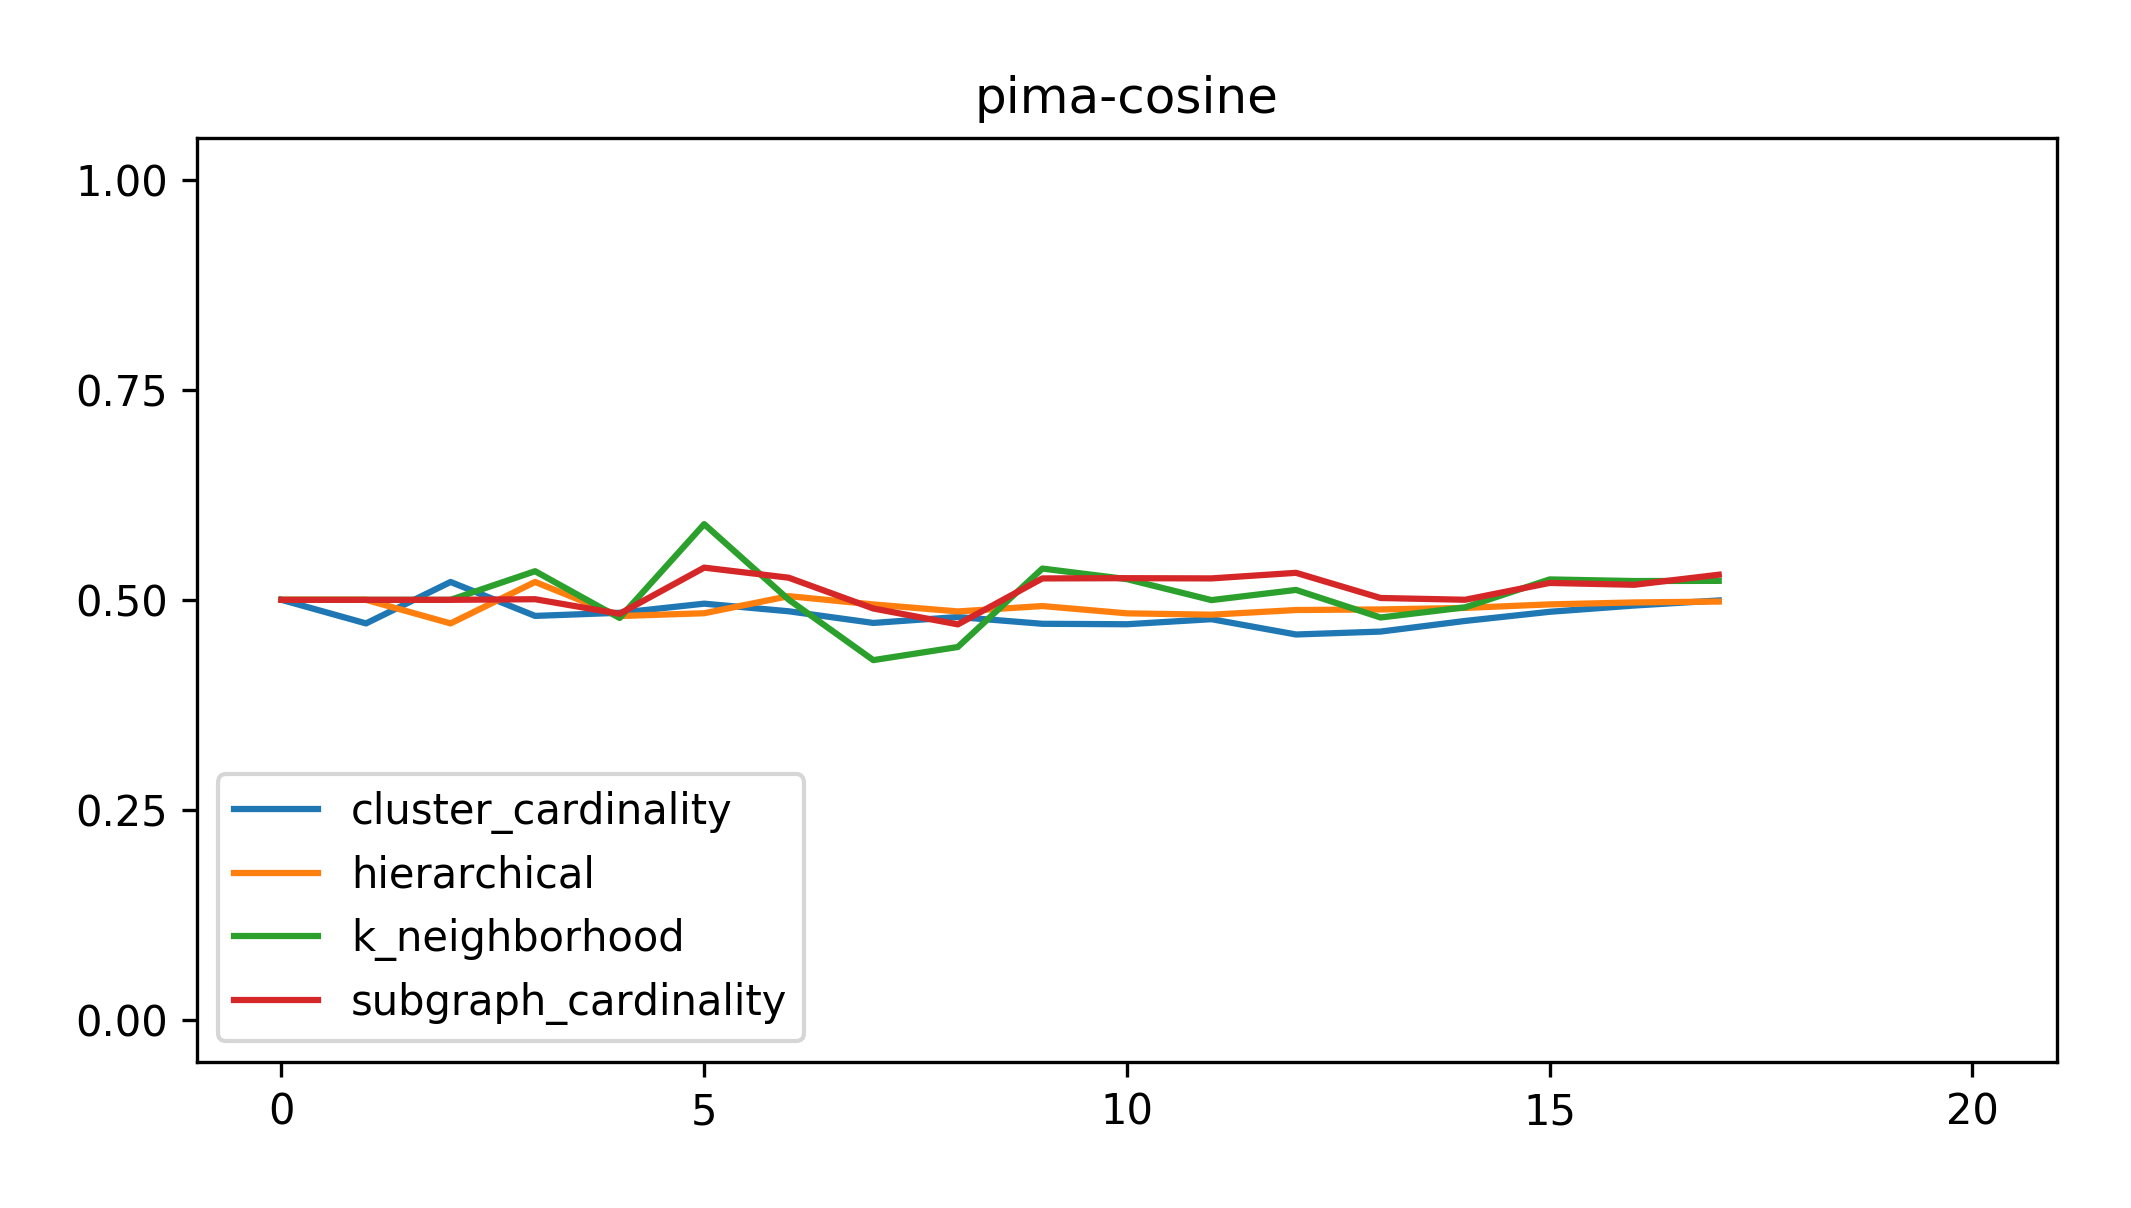
\includegraphics[width=2.2in]{kdd/static/auc_vs_depth/pima-cosine.png}
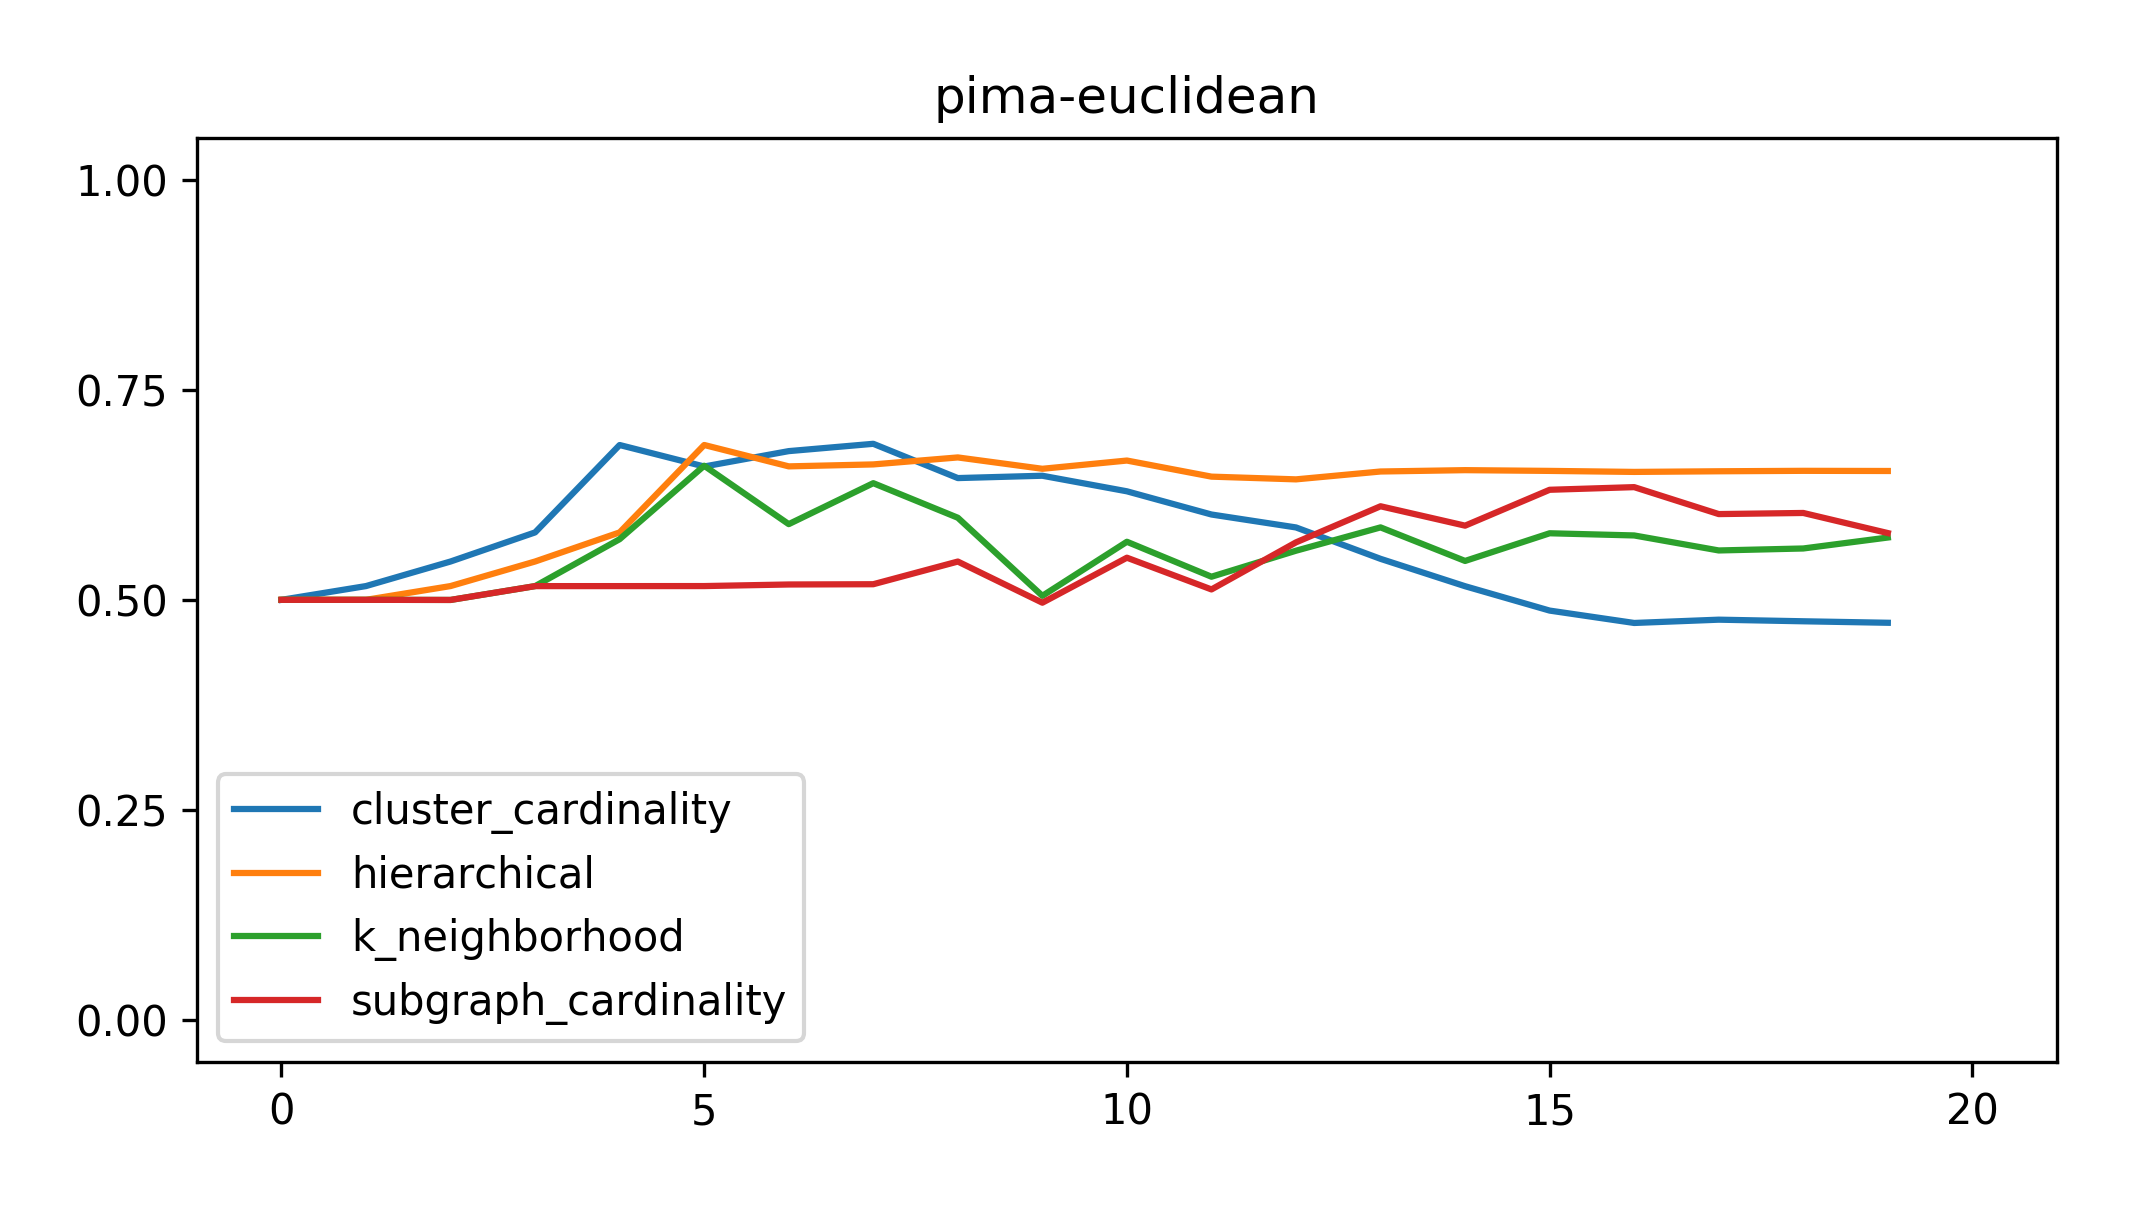
\includegraphics[width=2.2in]{kdd/static/auc_vs_depth/pima-euclidean.png}
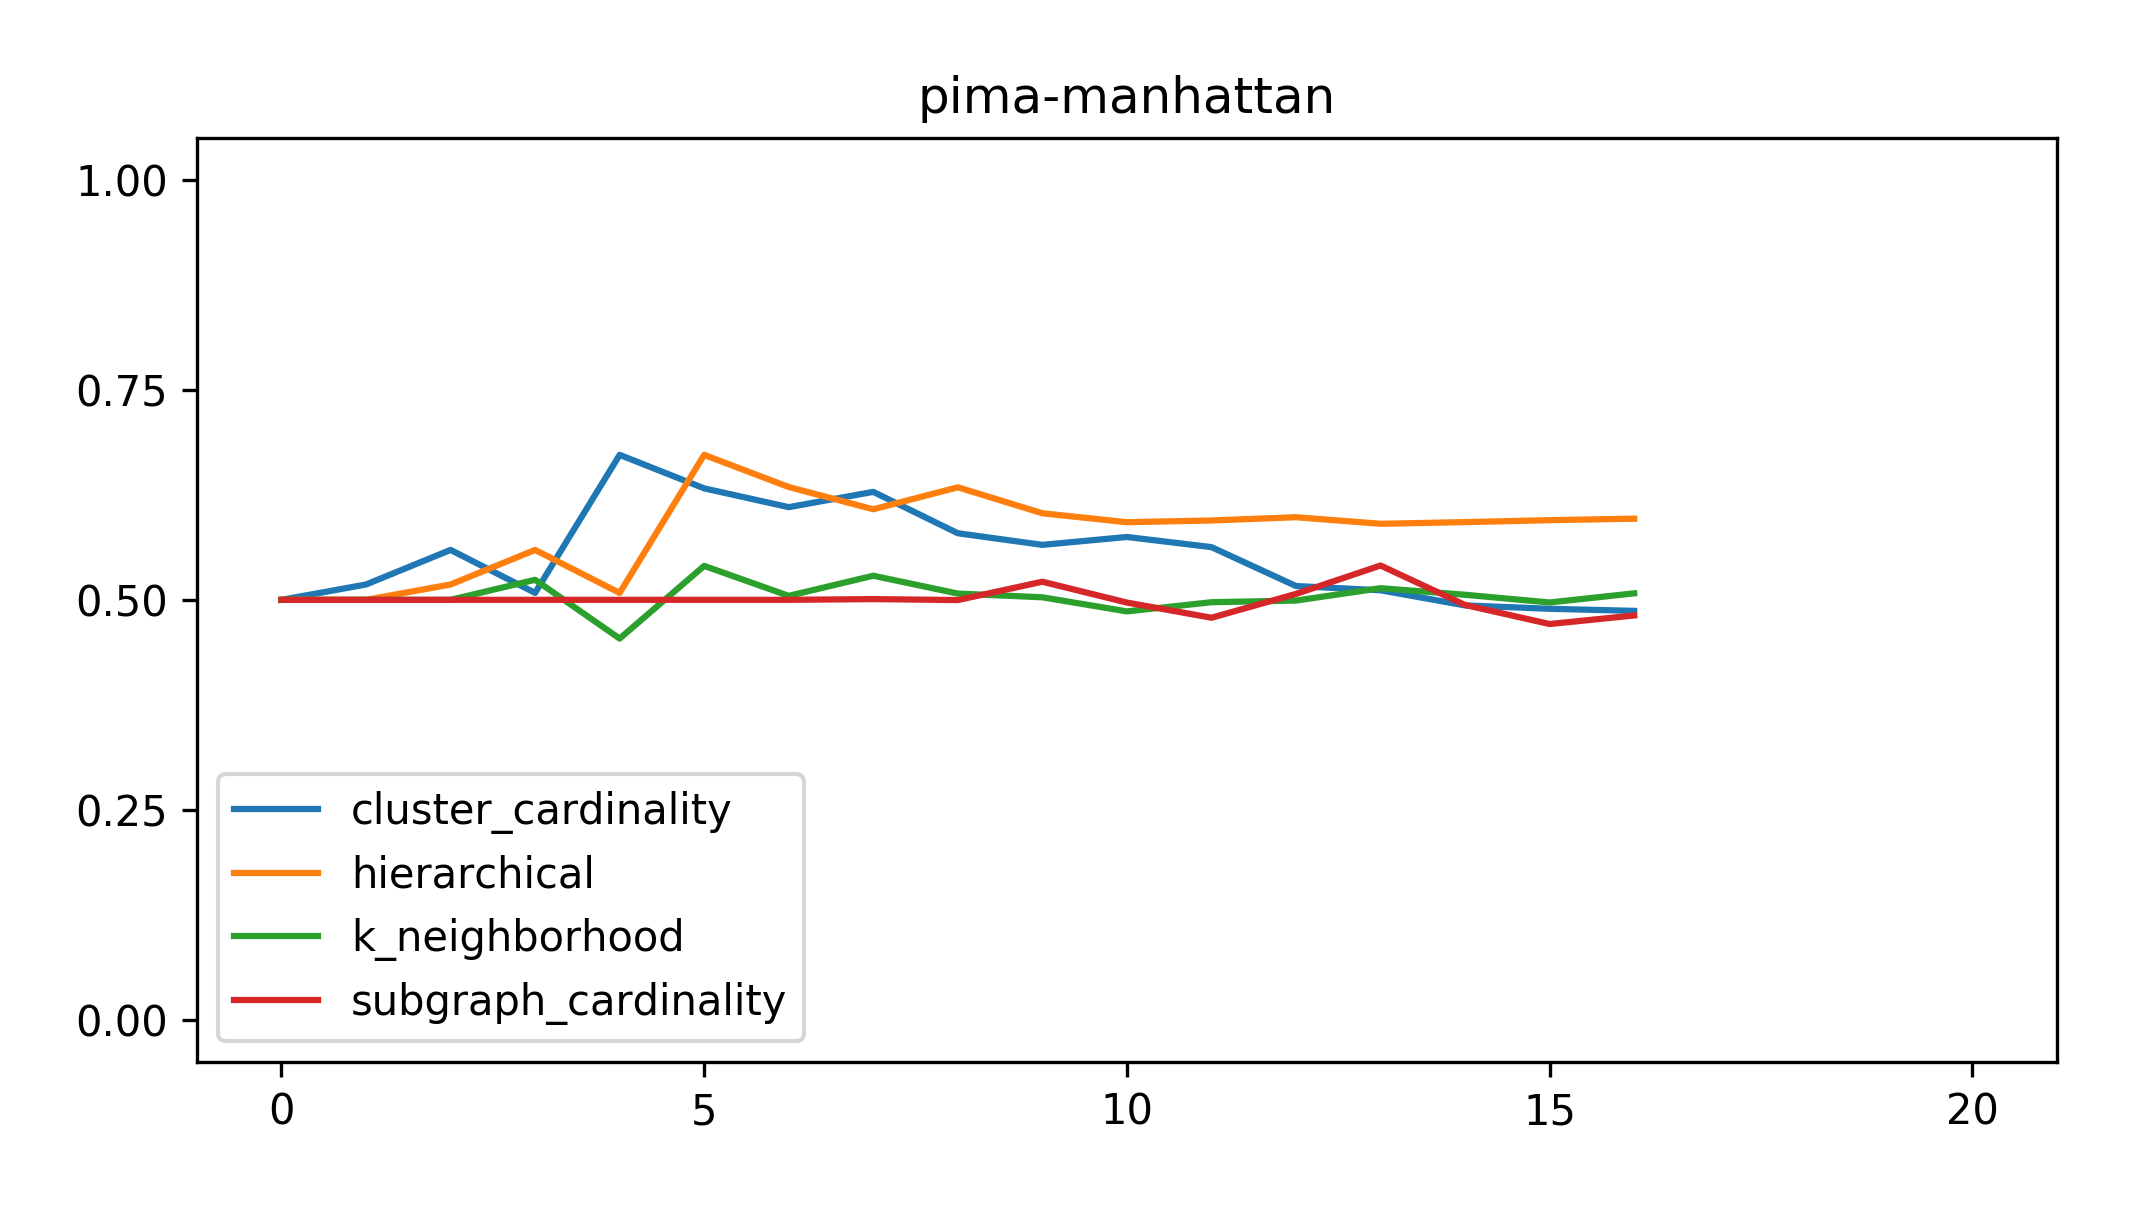
\includegraphics[width=2.2in]{kdd/static/auc_vs_depth/pima-manhattan.png}

% Satellite
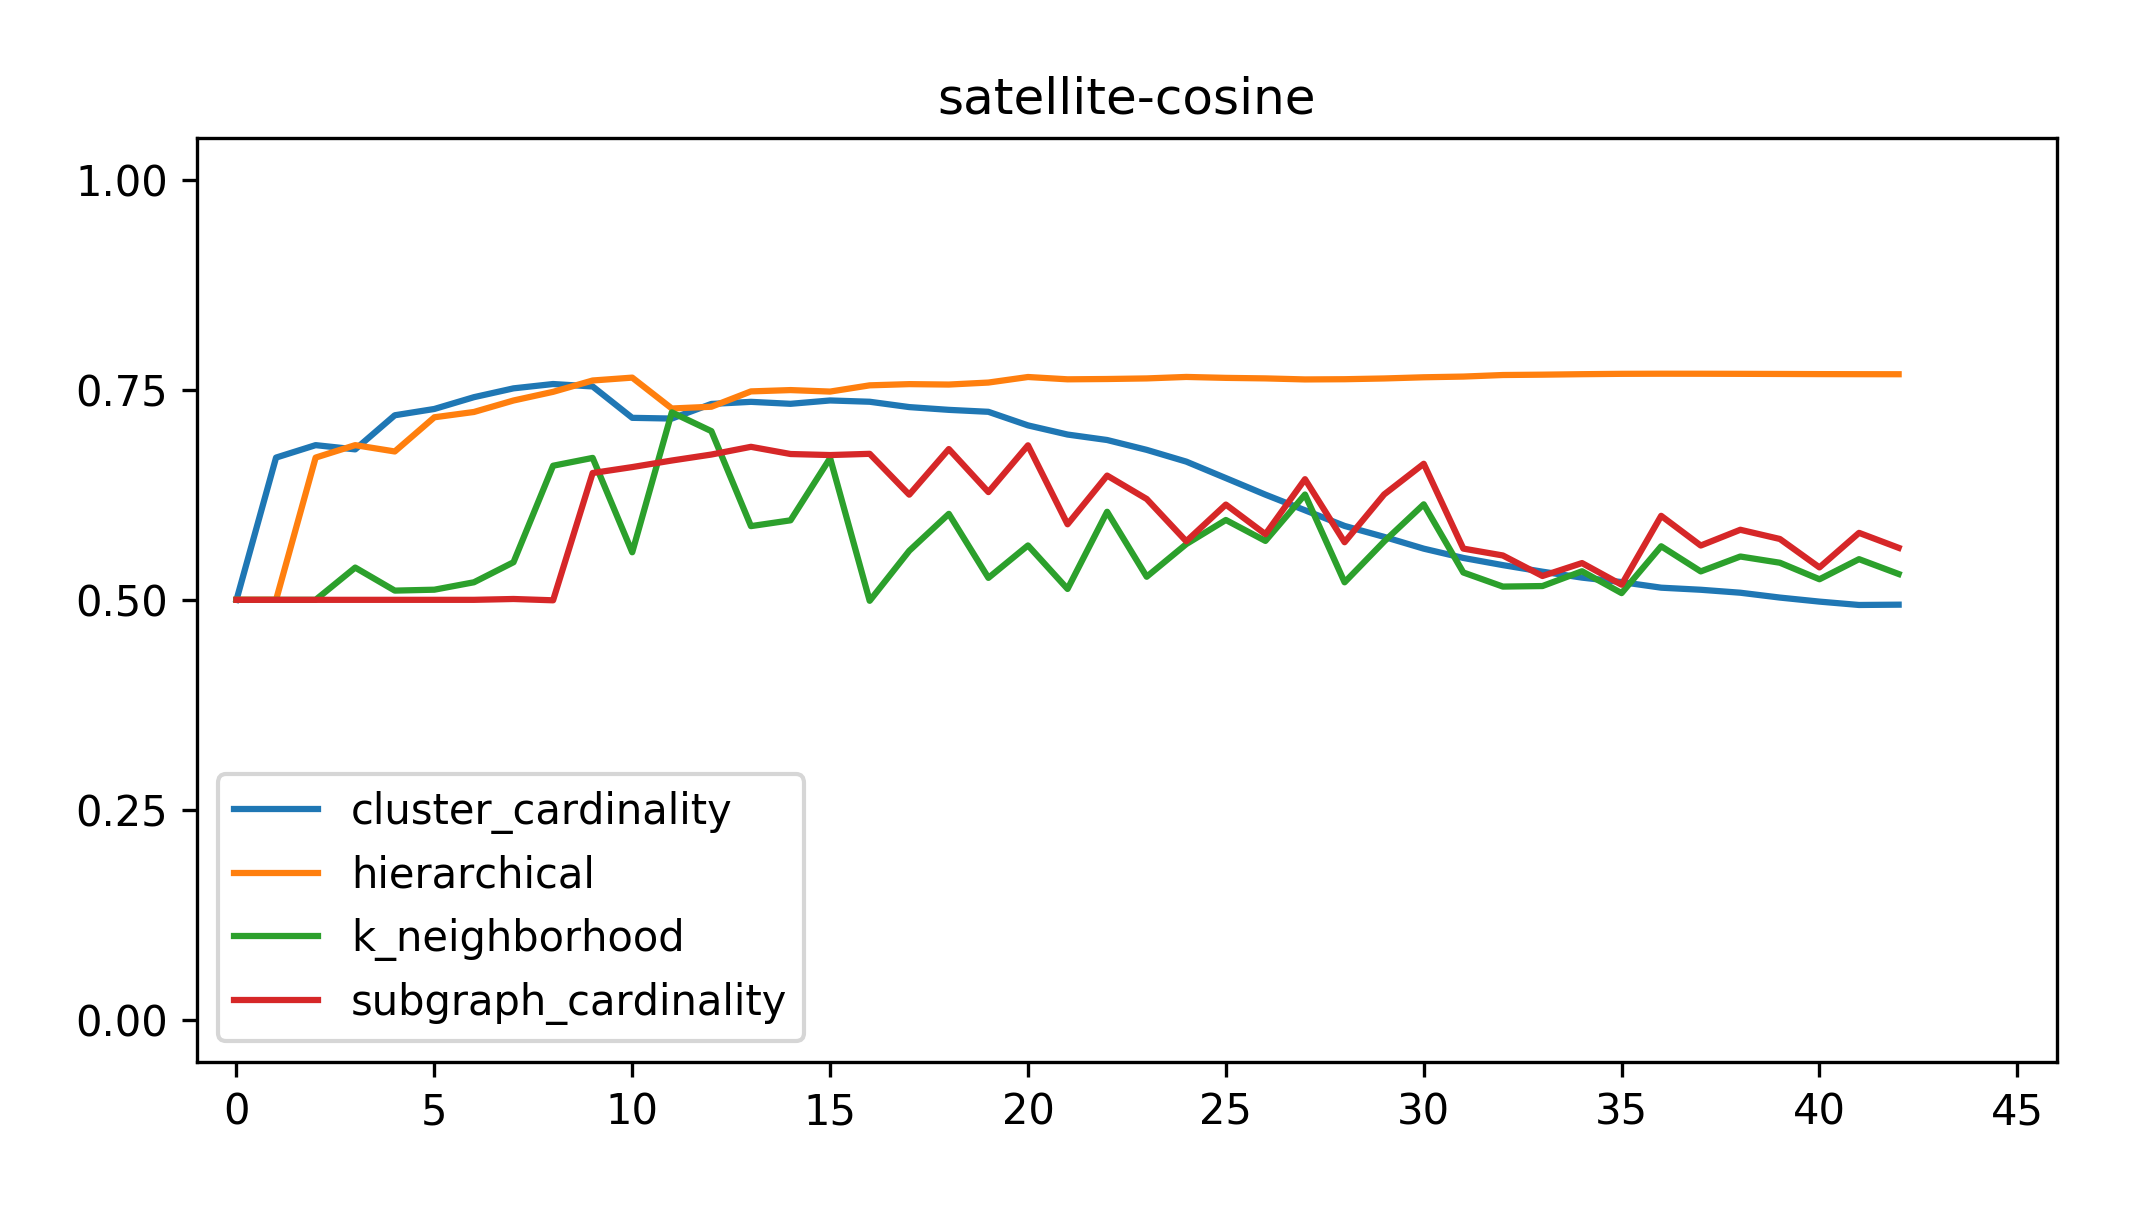
\includegraphics[width=2.2in]{kdd/static/auc_vs_depth/satellite-cosine.png}
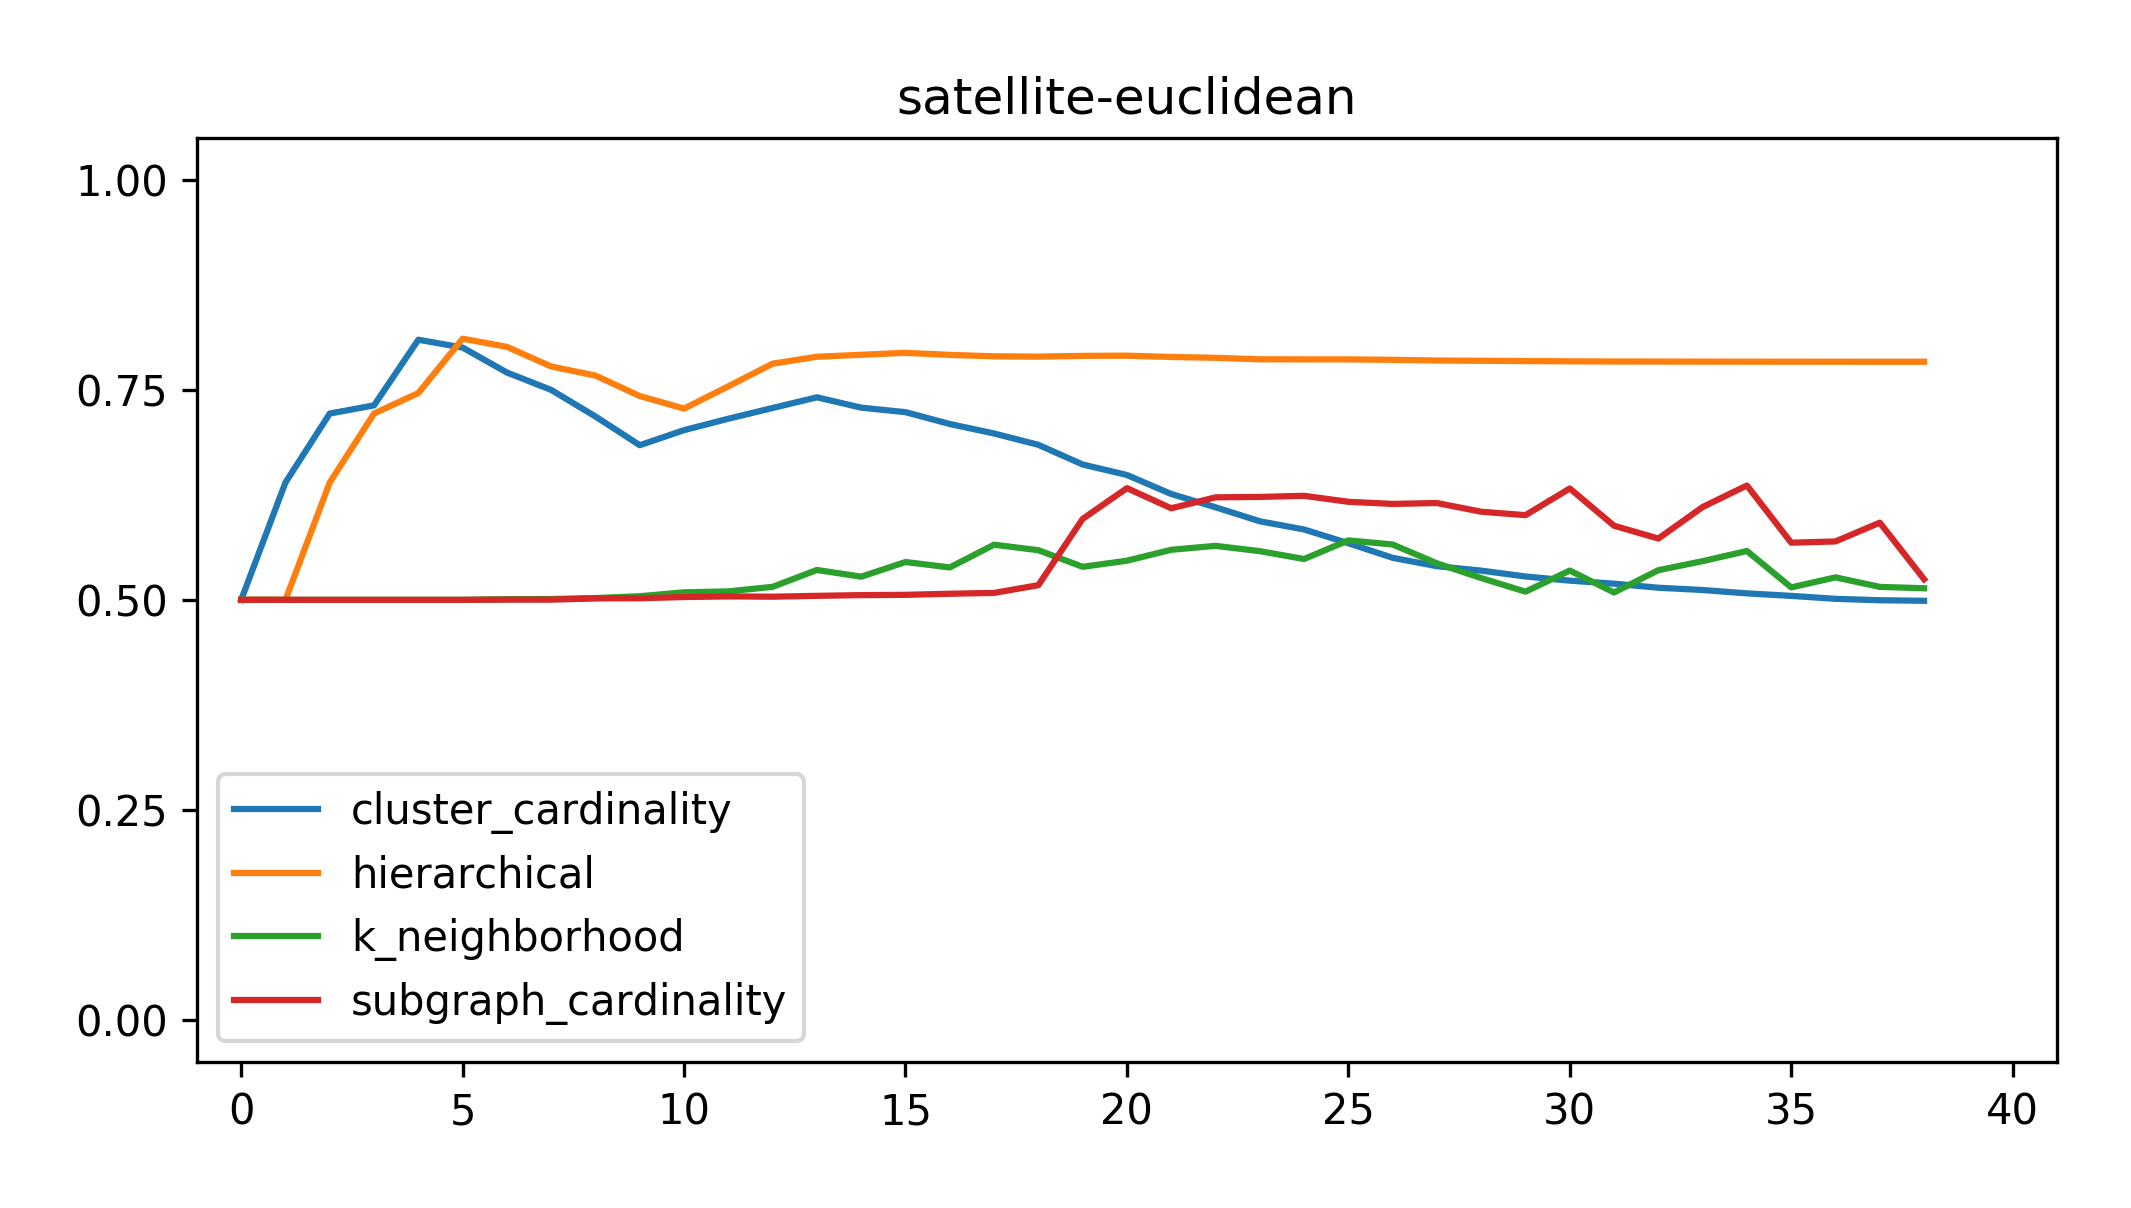
\includegraphics[width=2.2in]{kdd/static/auc_vs_depth/satellite-euclidean.png}
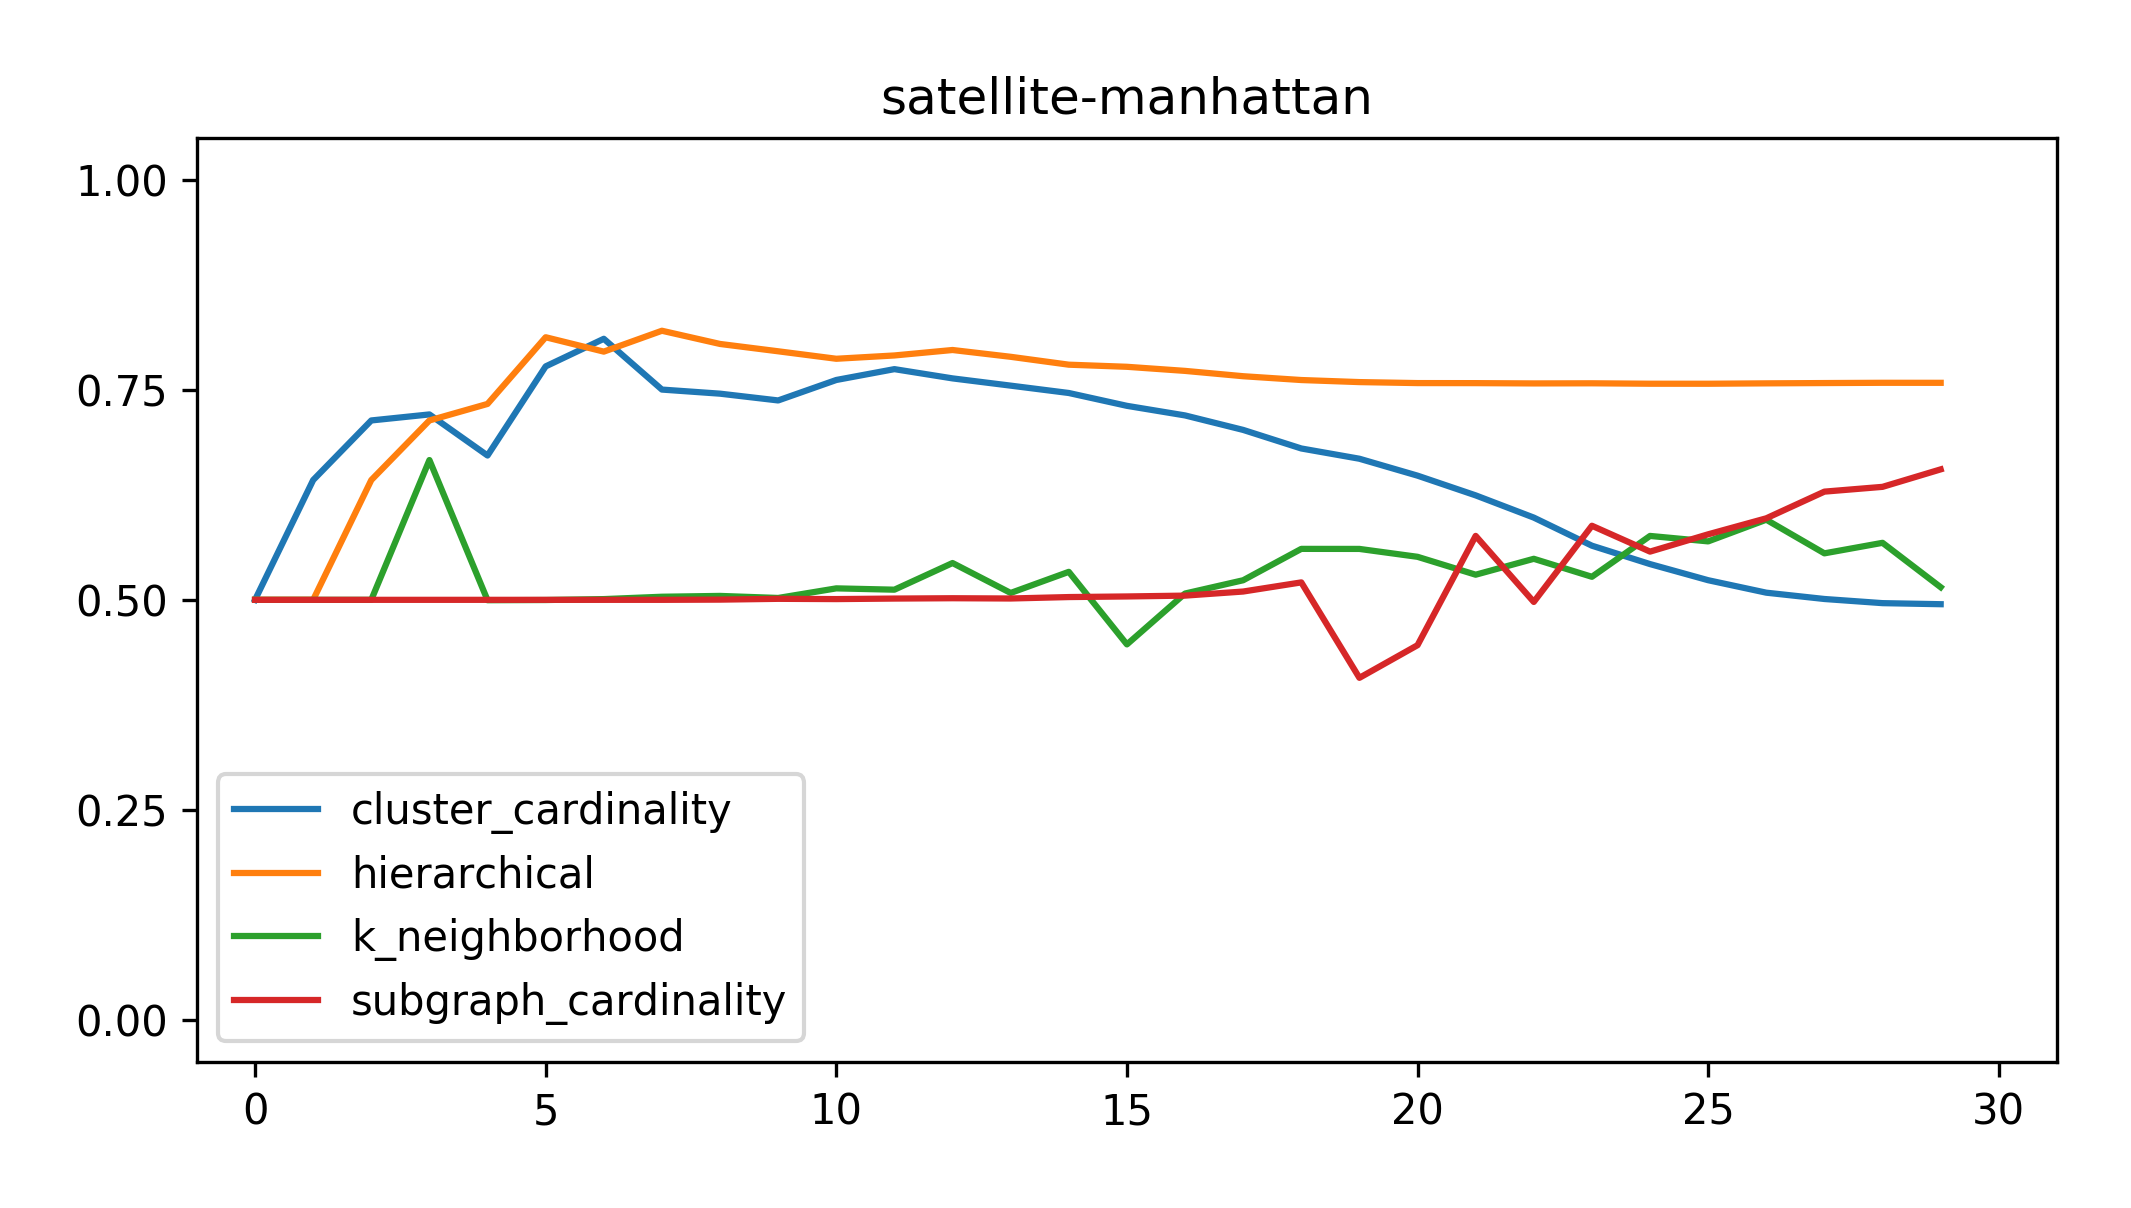
\includegraphics[width=2.2in]{kdd/static/auc_vs_depth/satellite-manhattan.png}

\caption{
Plots of ROC-AUC vs Depth for our mearures of Anomolousness.
}

\label{results:datasets_2}
\end{figure*}

\begin{figure*}[!t]
\centering
% Satimage-2
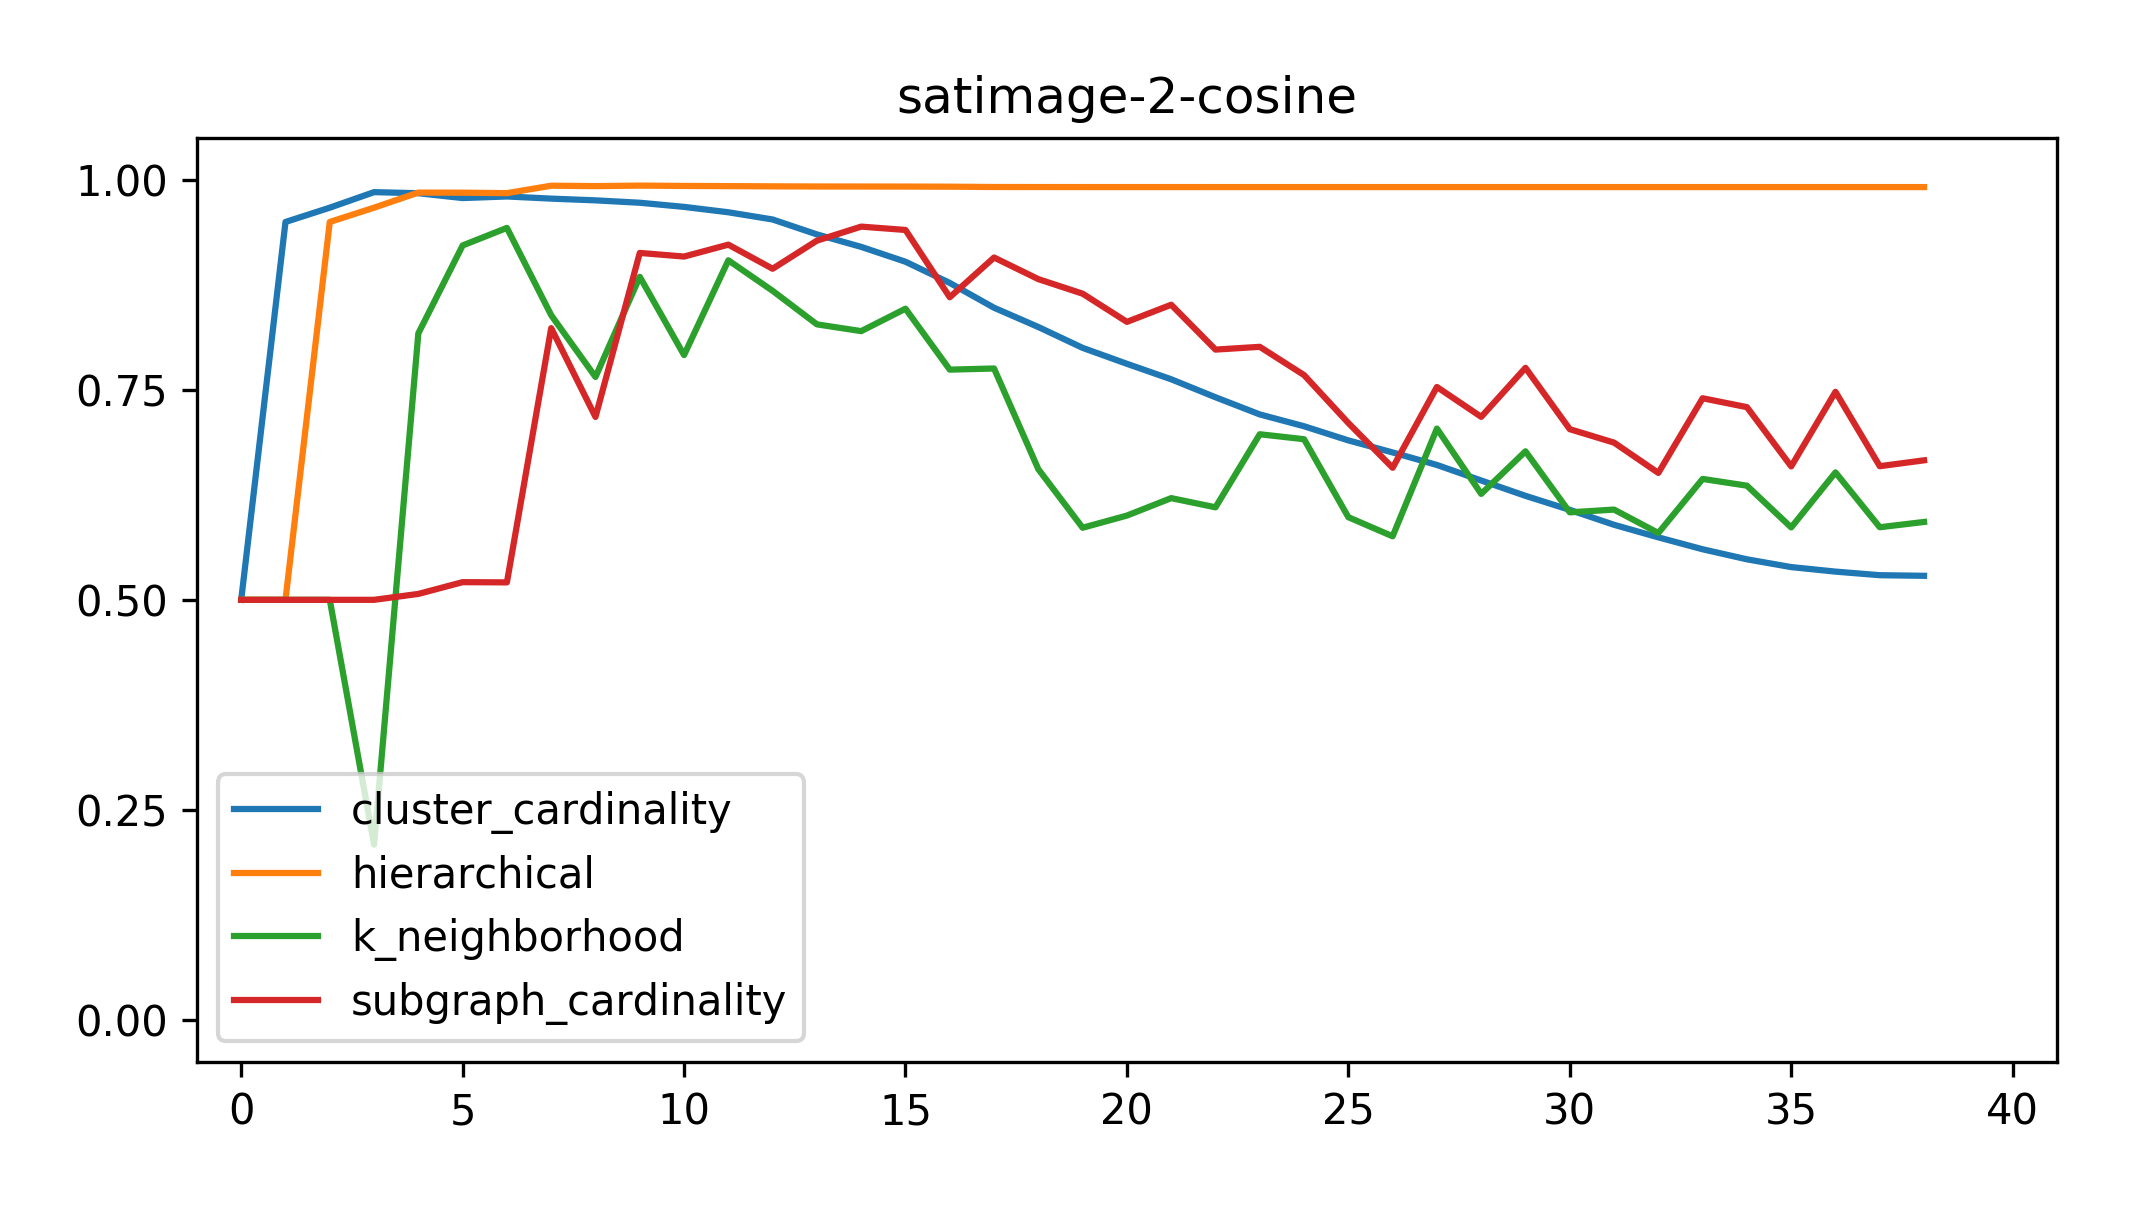
\includegraphics[width=2.2in]{kdd/static/auc_vs_depth/satimage-2-cosine.png}
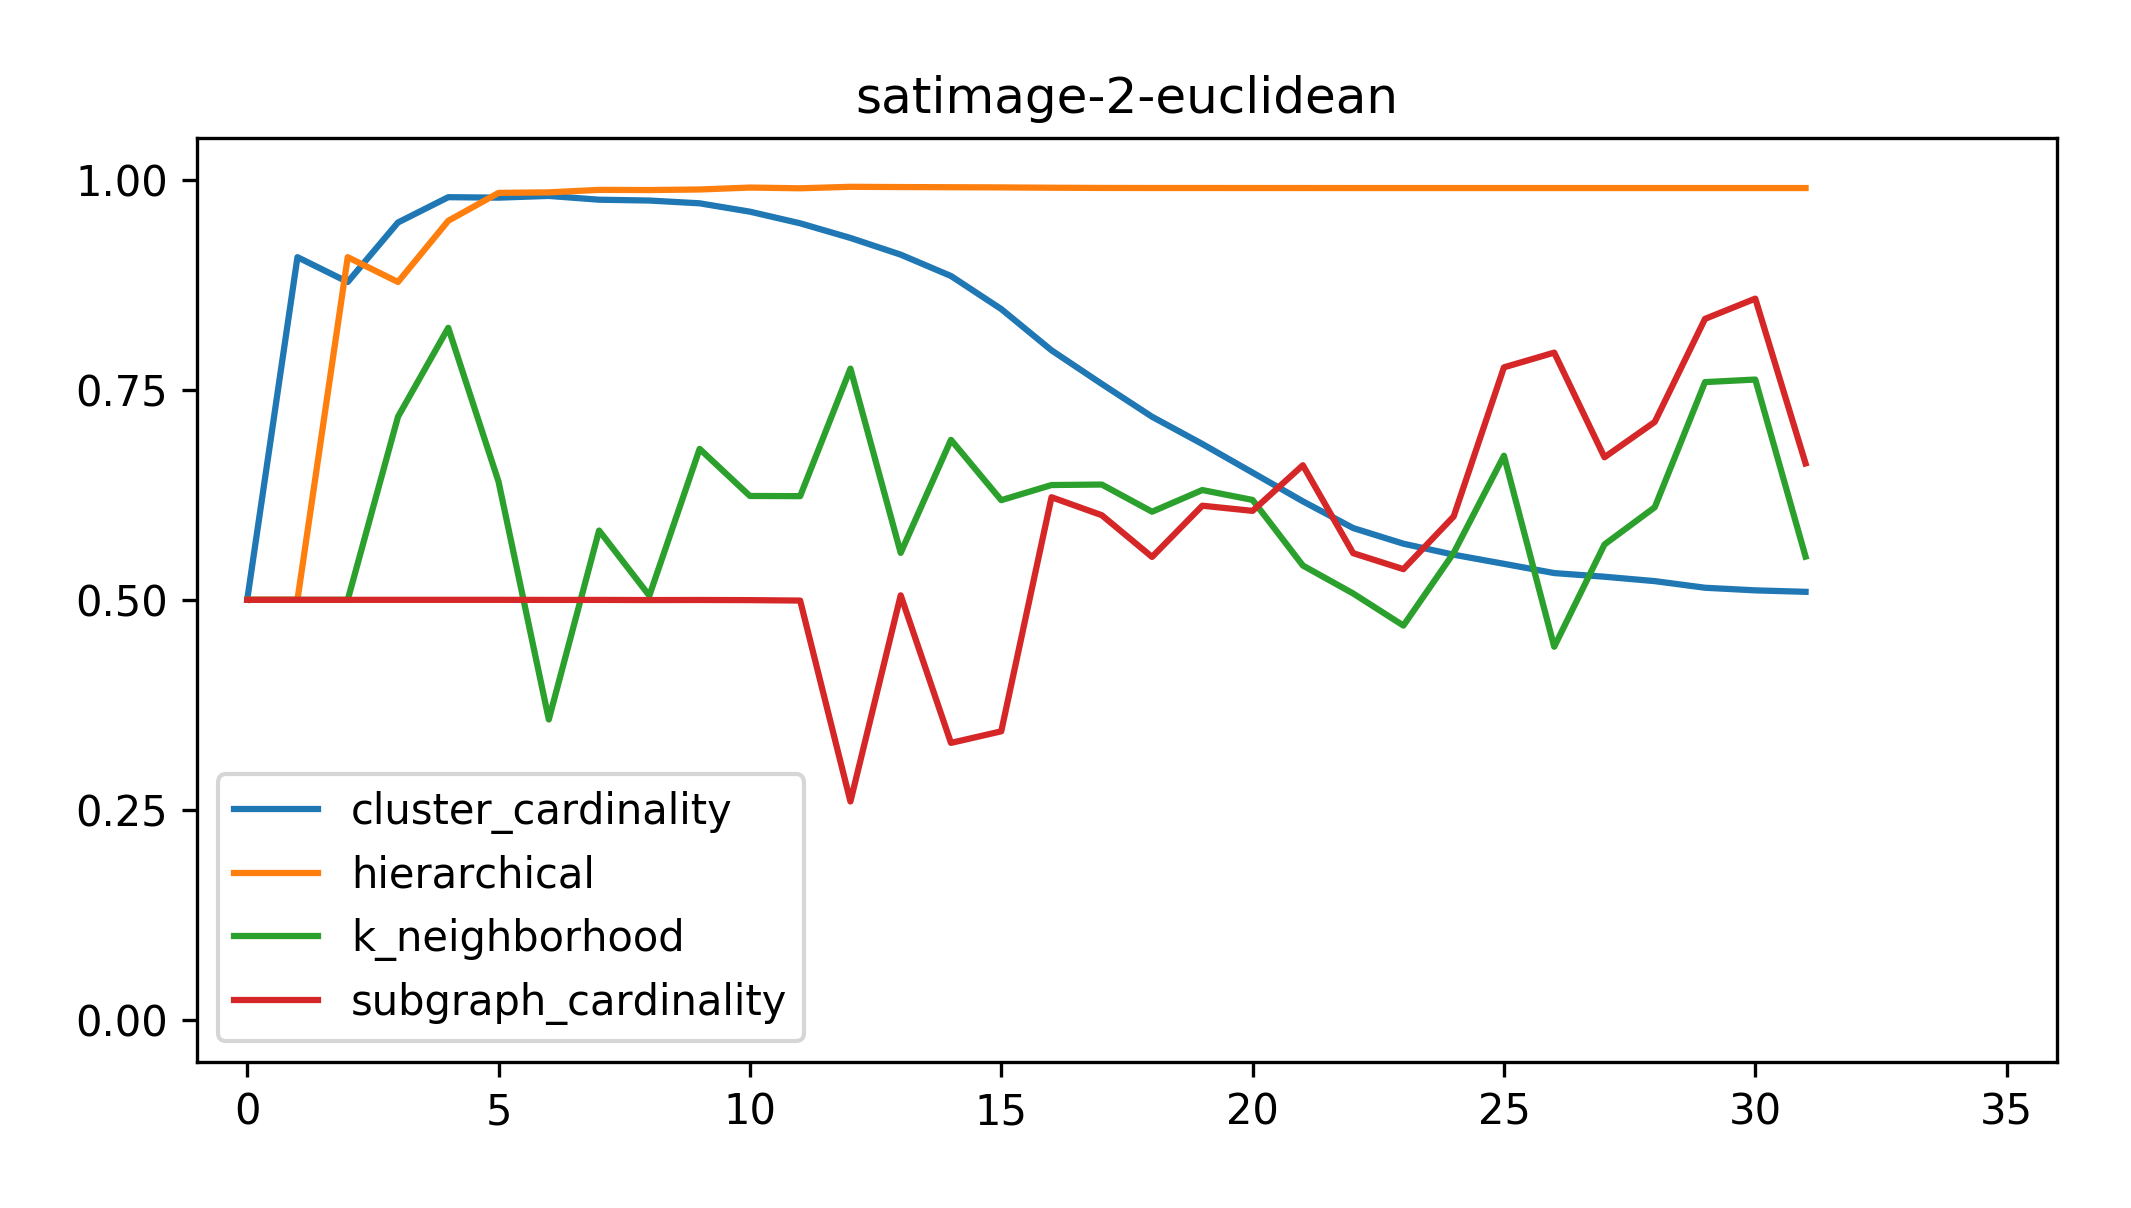
\includegraphics[width=2.2in]{kdd/static/auc_vs_depth/satimage-2-euclidean.png}
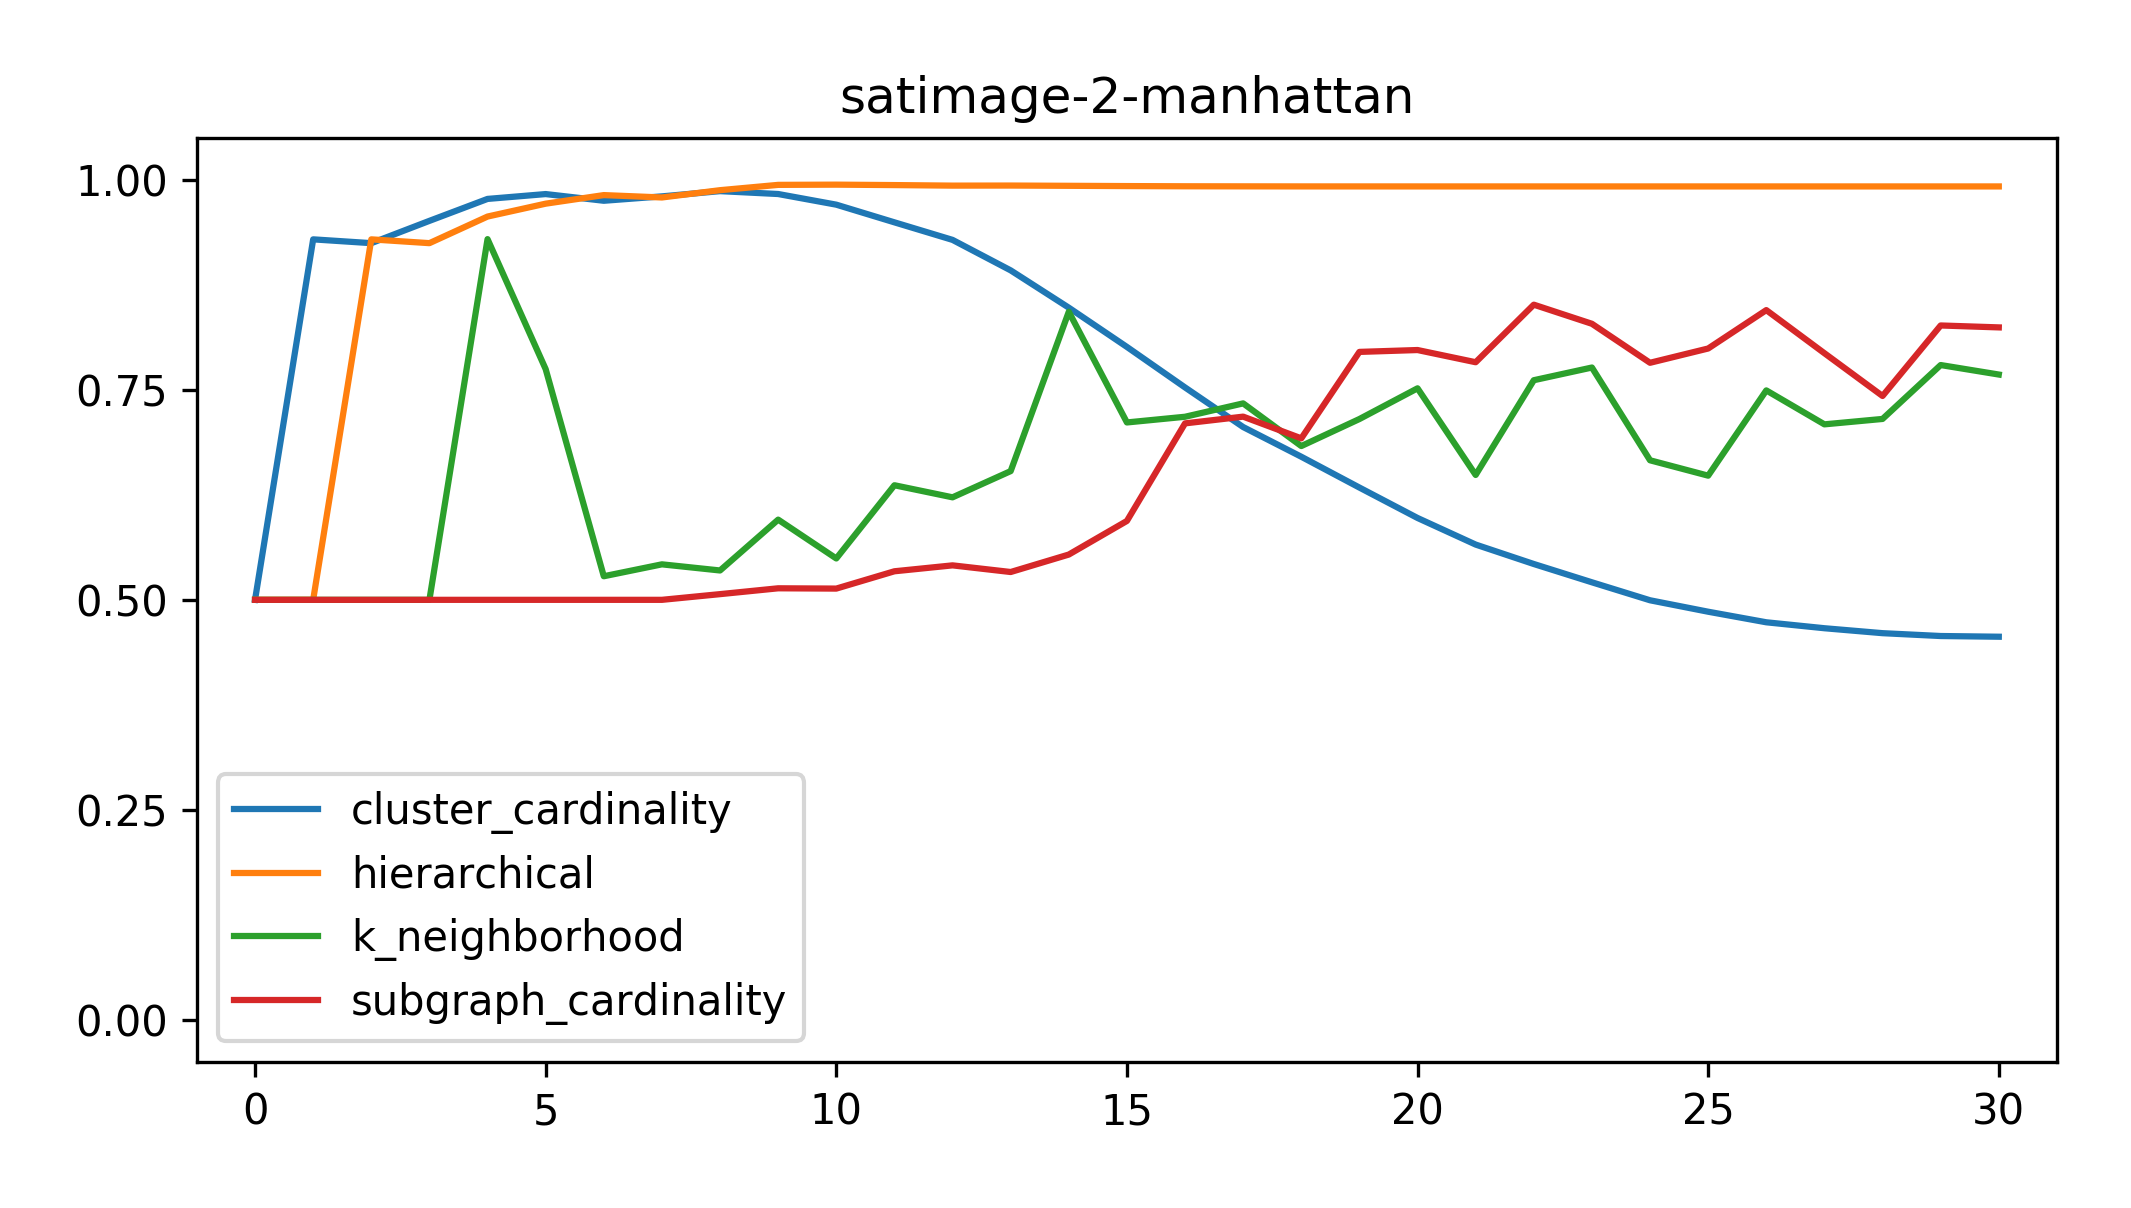
\includegraphics[width=2.2in]{kdd/static/auc_vs_depth/satimage-2-manhattan.png}

% Thyroid
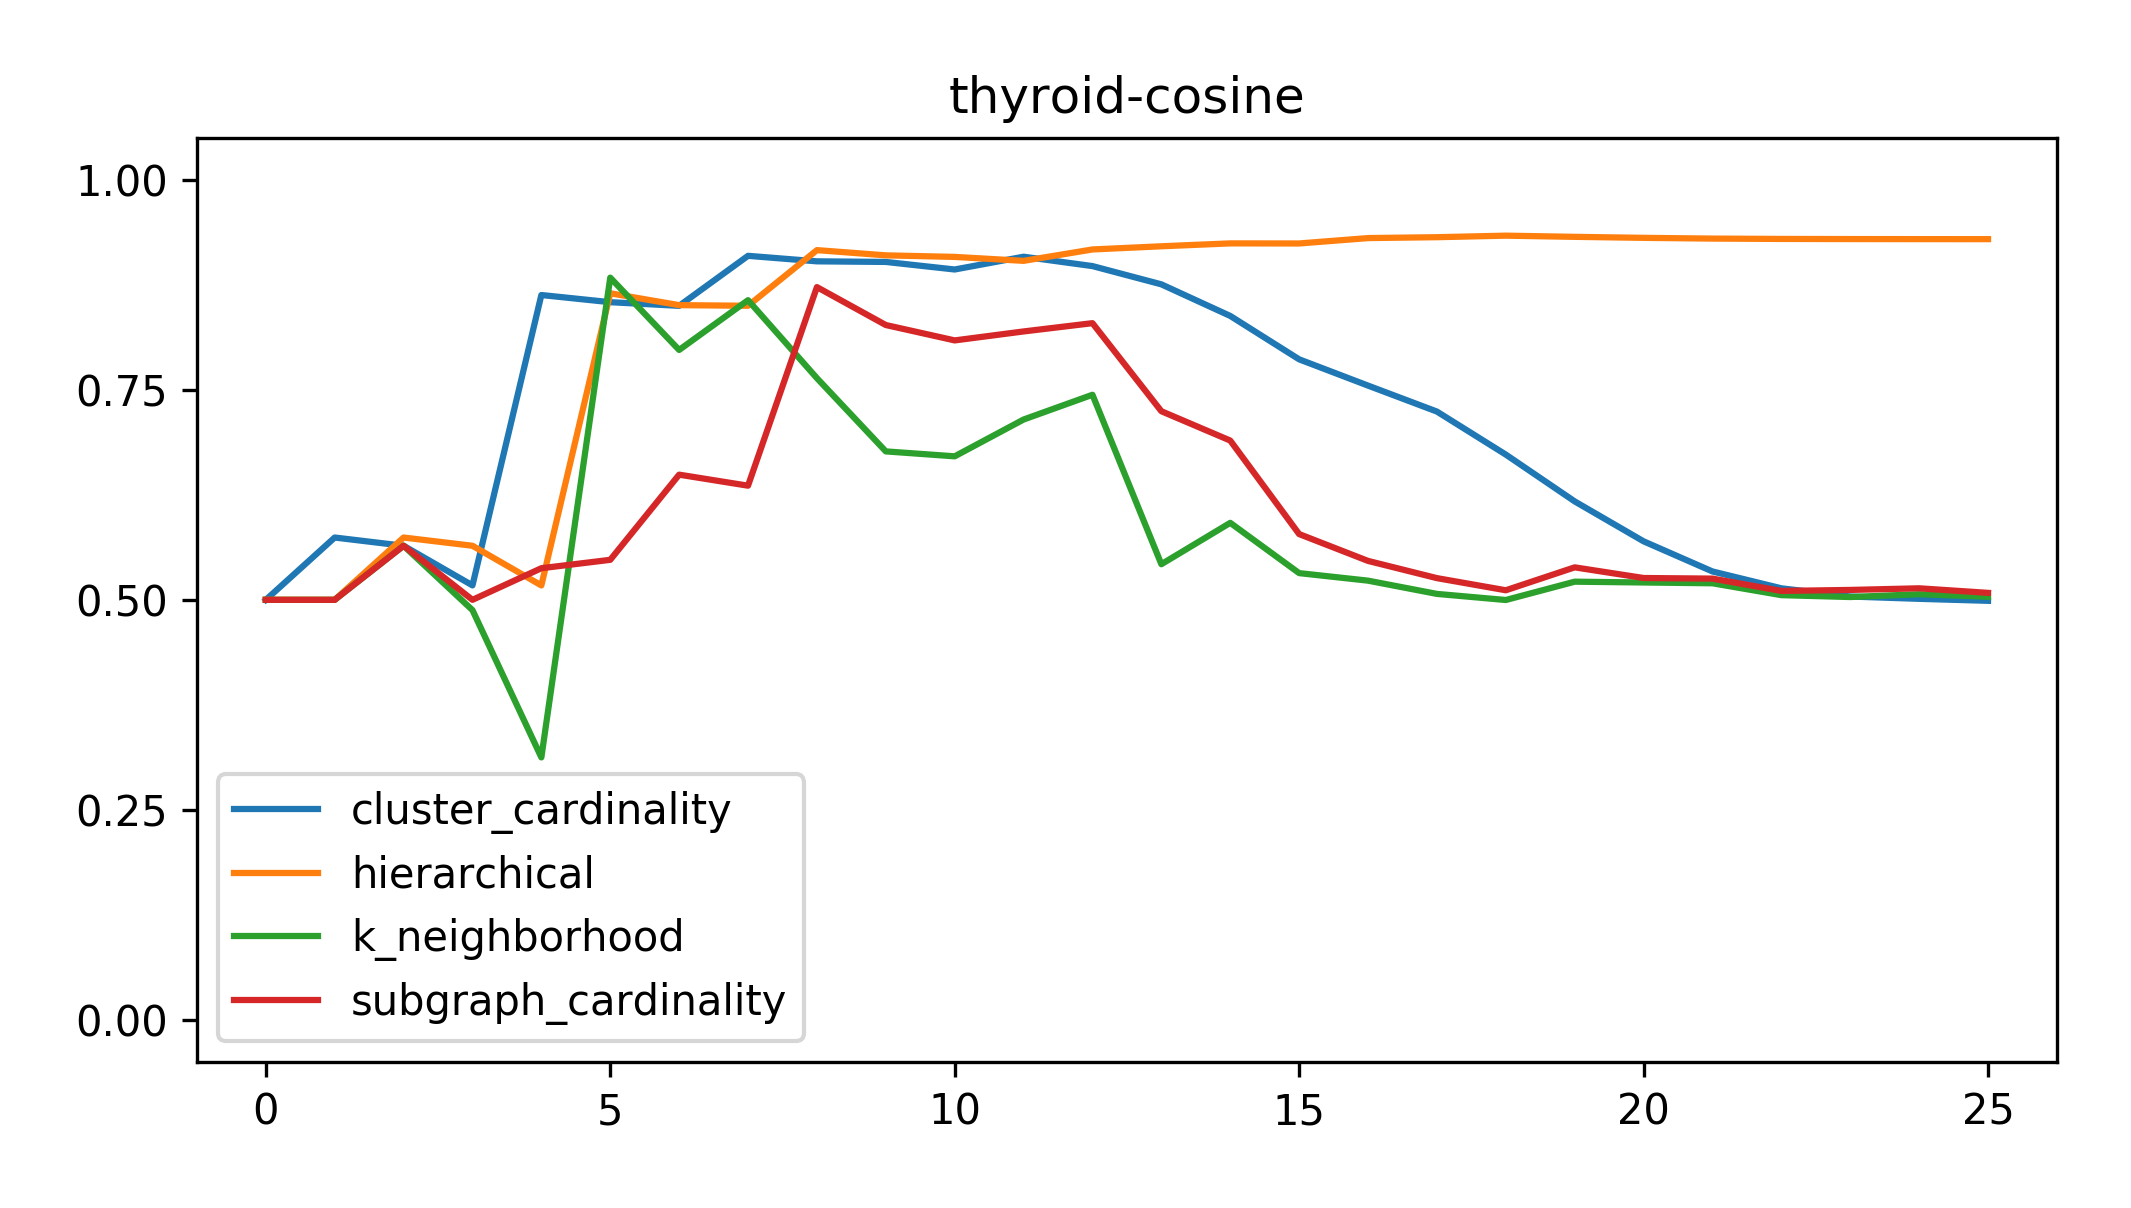
\includegraphics[width=2.2in]{kdd/static/auc_vs_depth/thyroid-cosine.png}
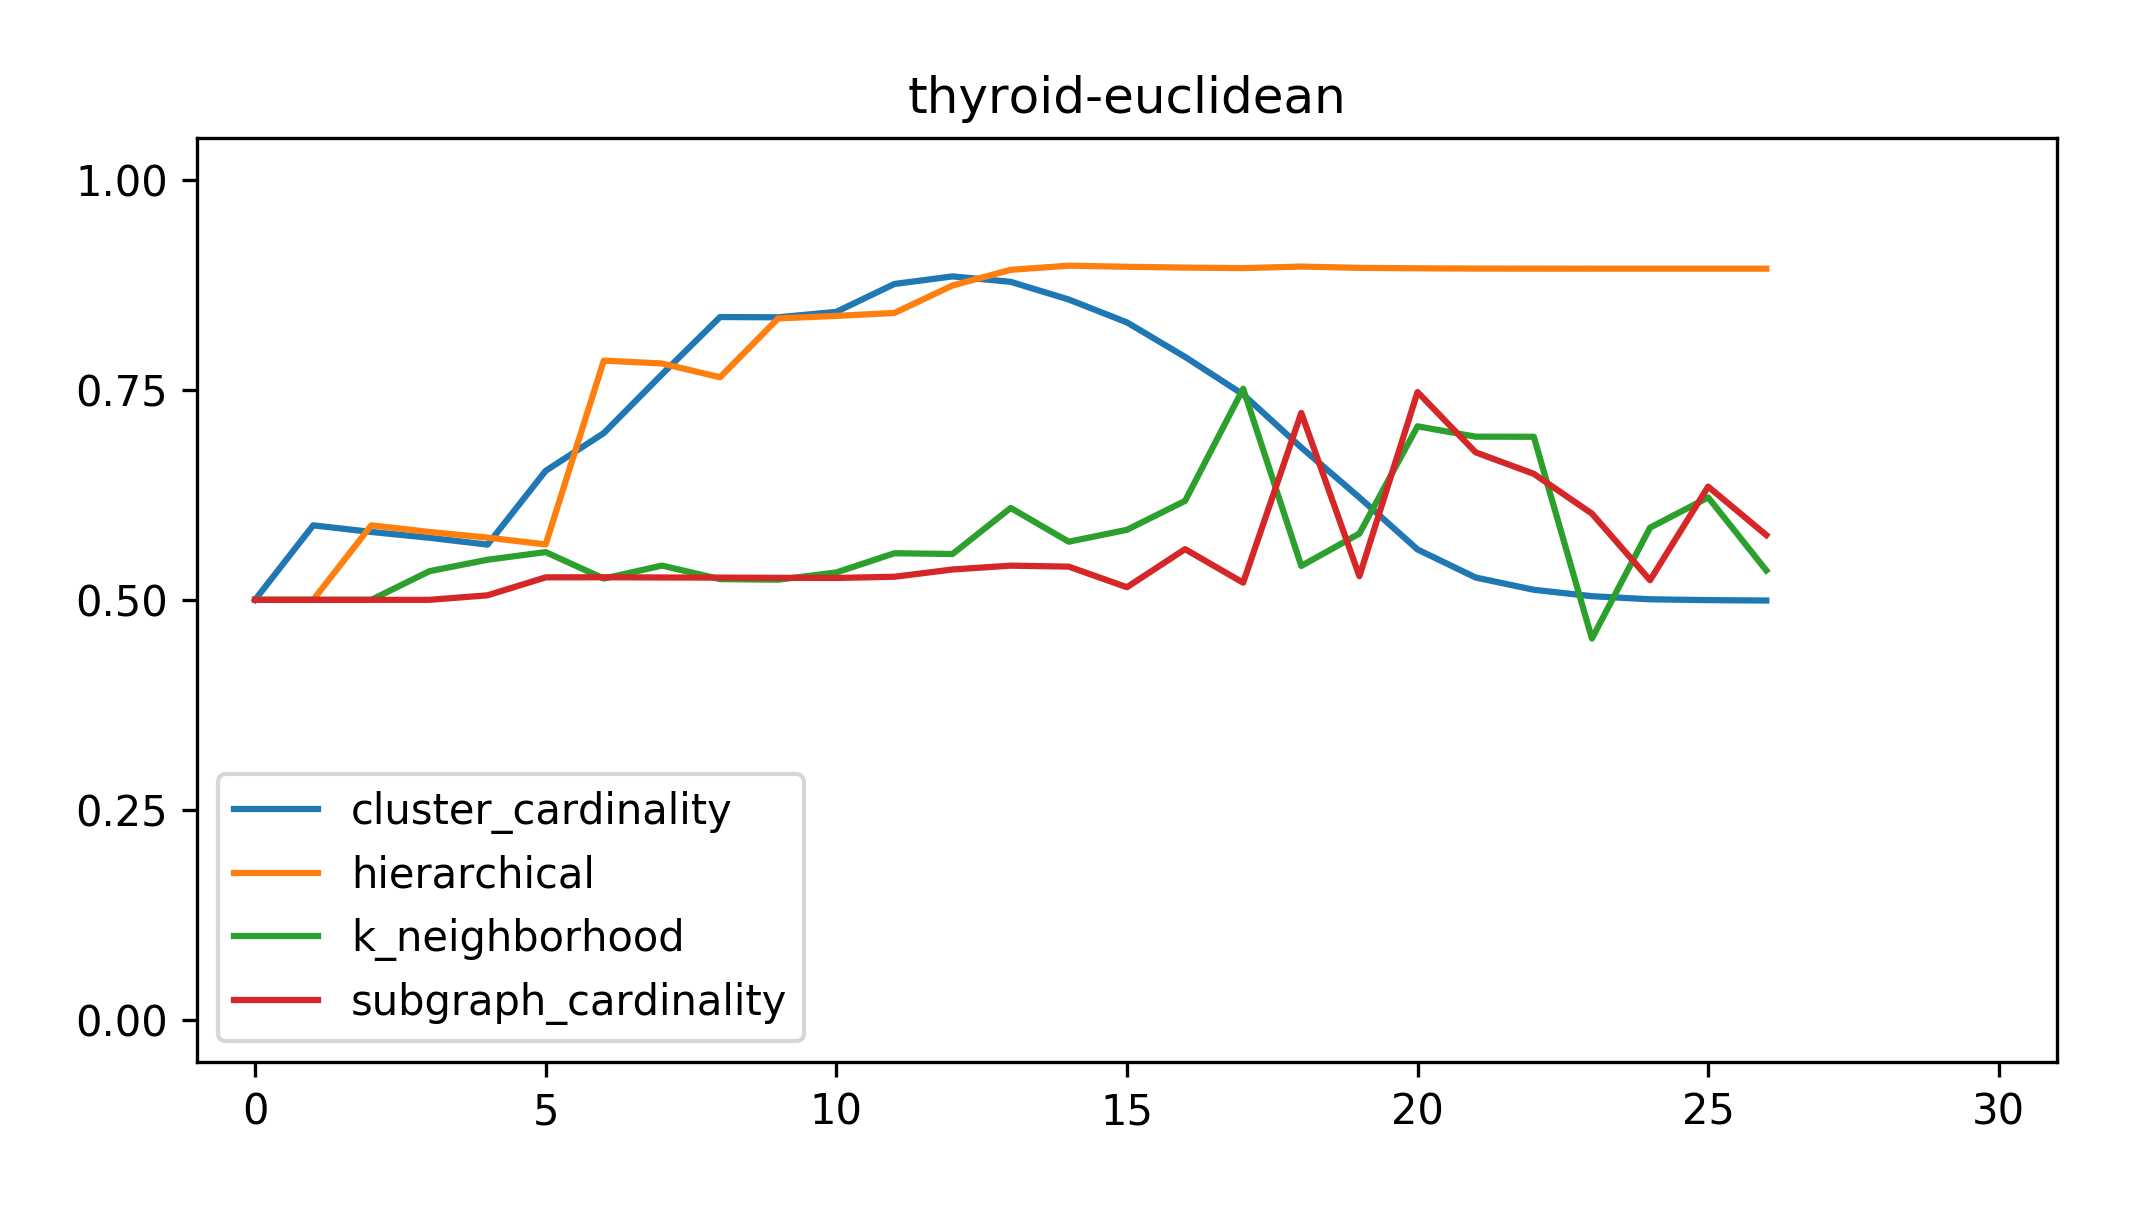
\includegraphics[width=2.2in]{kdd/static/auc_vs_depth/thyroid-euclidean.png}
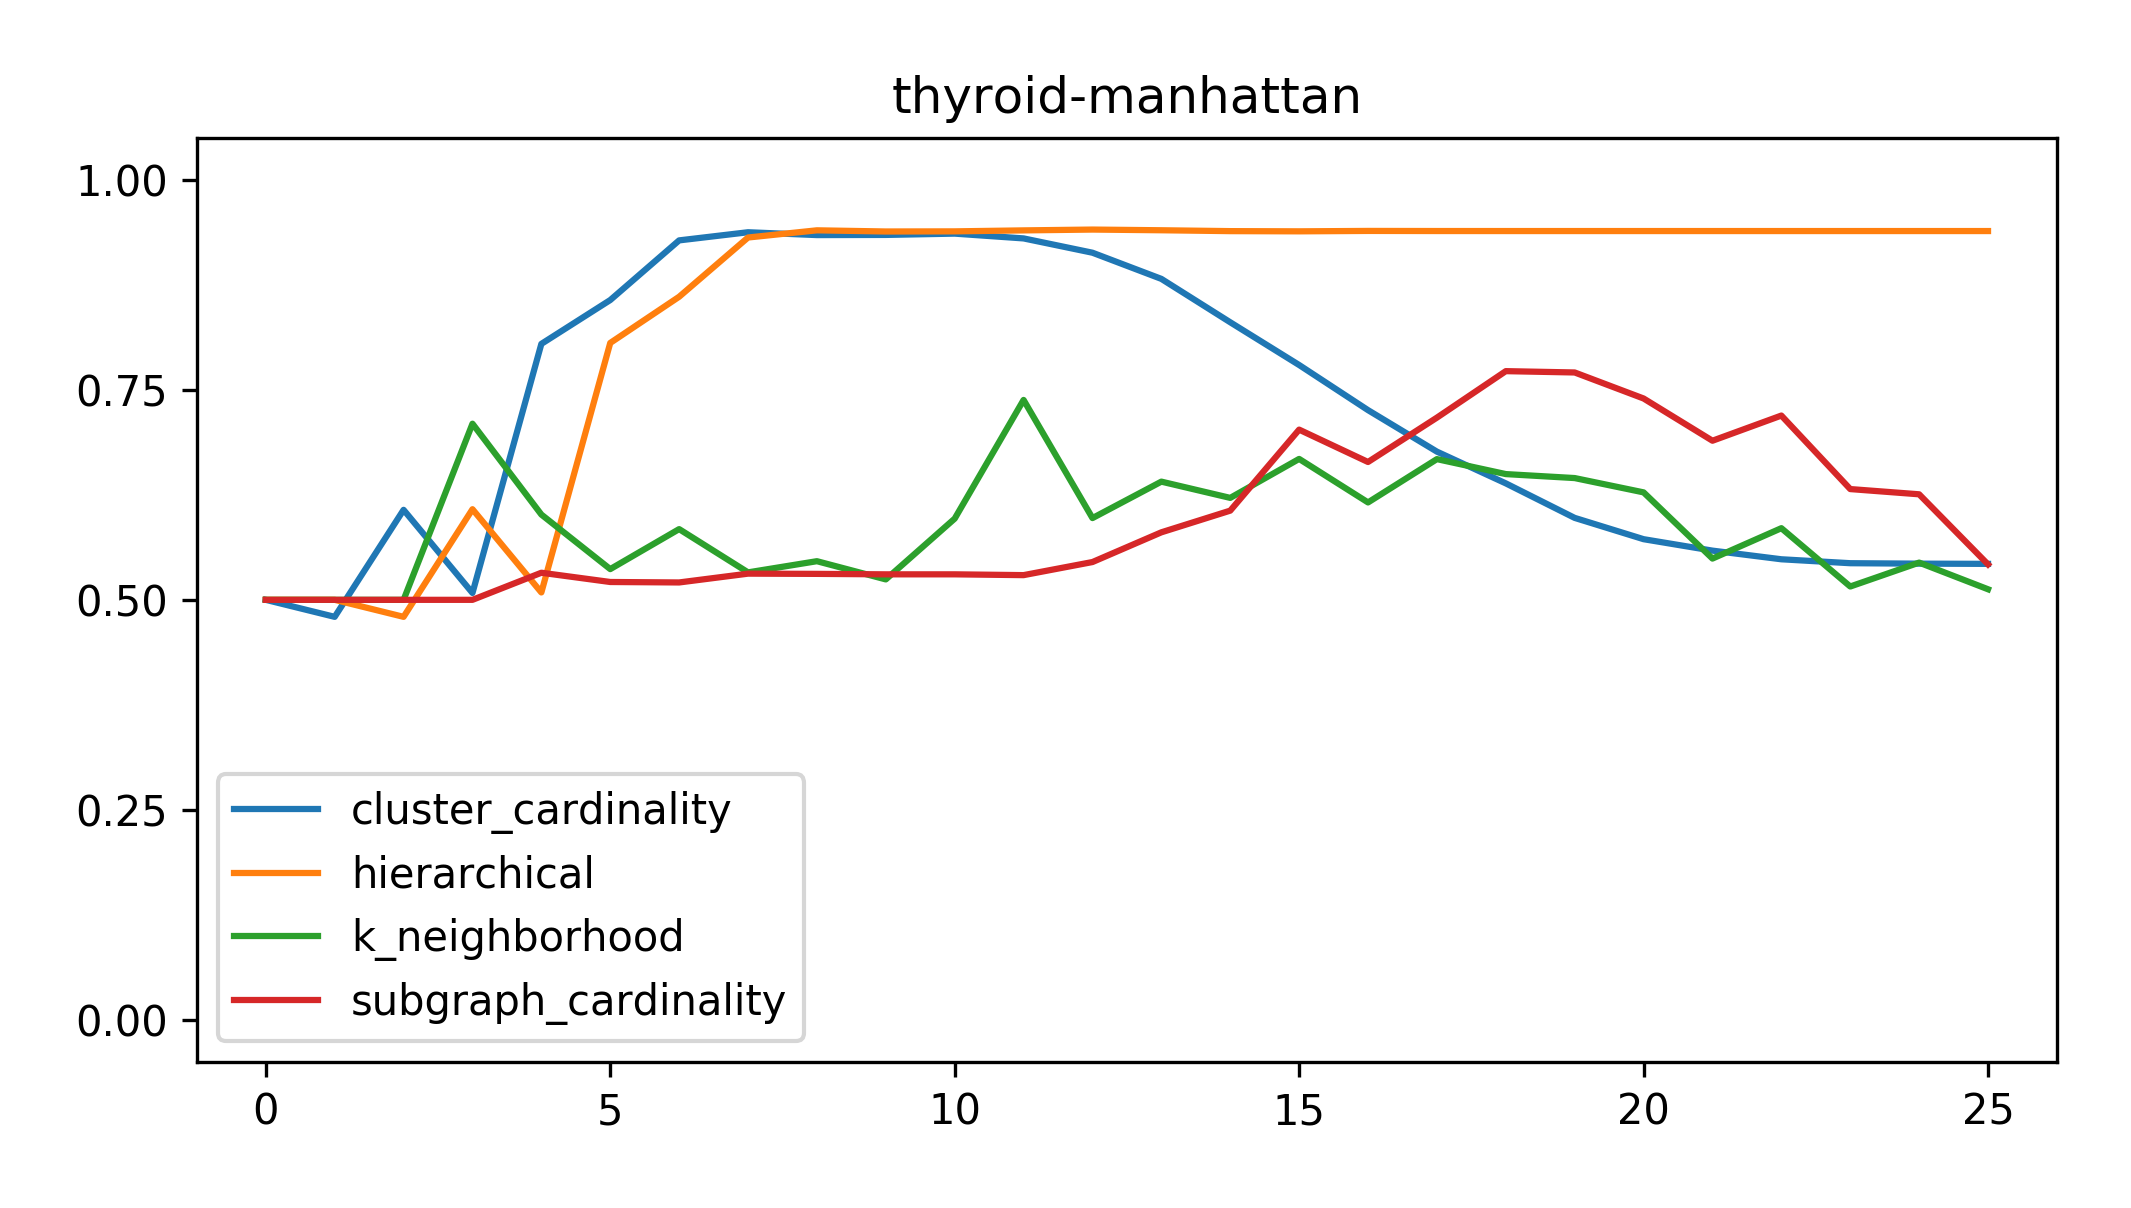
\includegraphics[width=2.2in]{kdd/static/auc_vs_depth/thyroid-manhattan.png}

% Vertebral
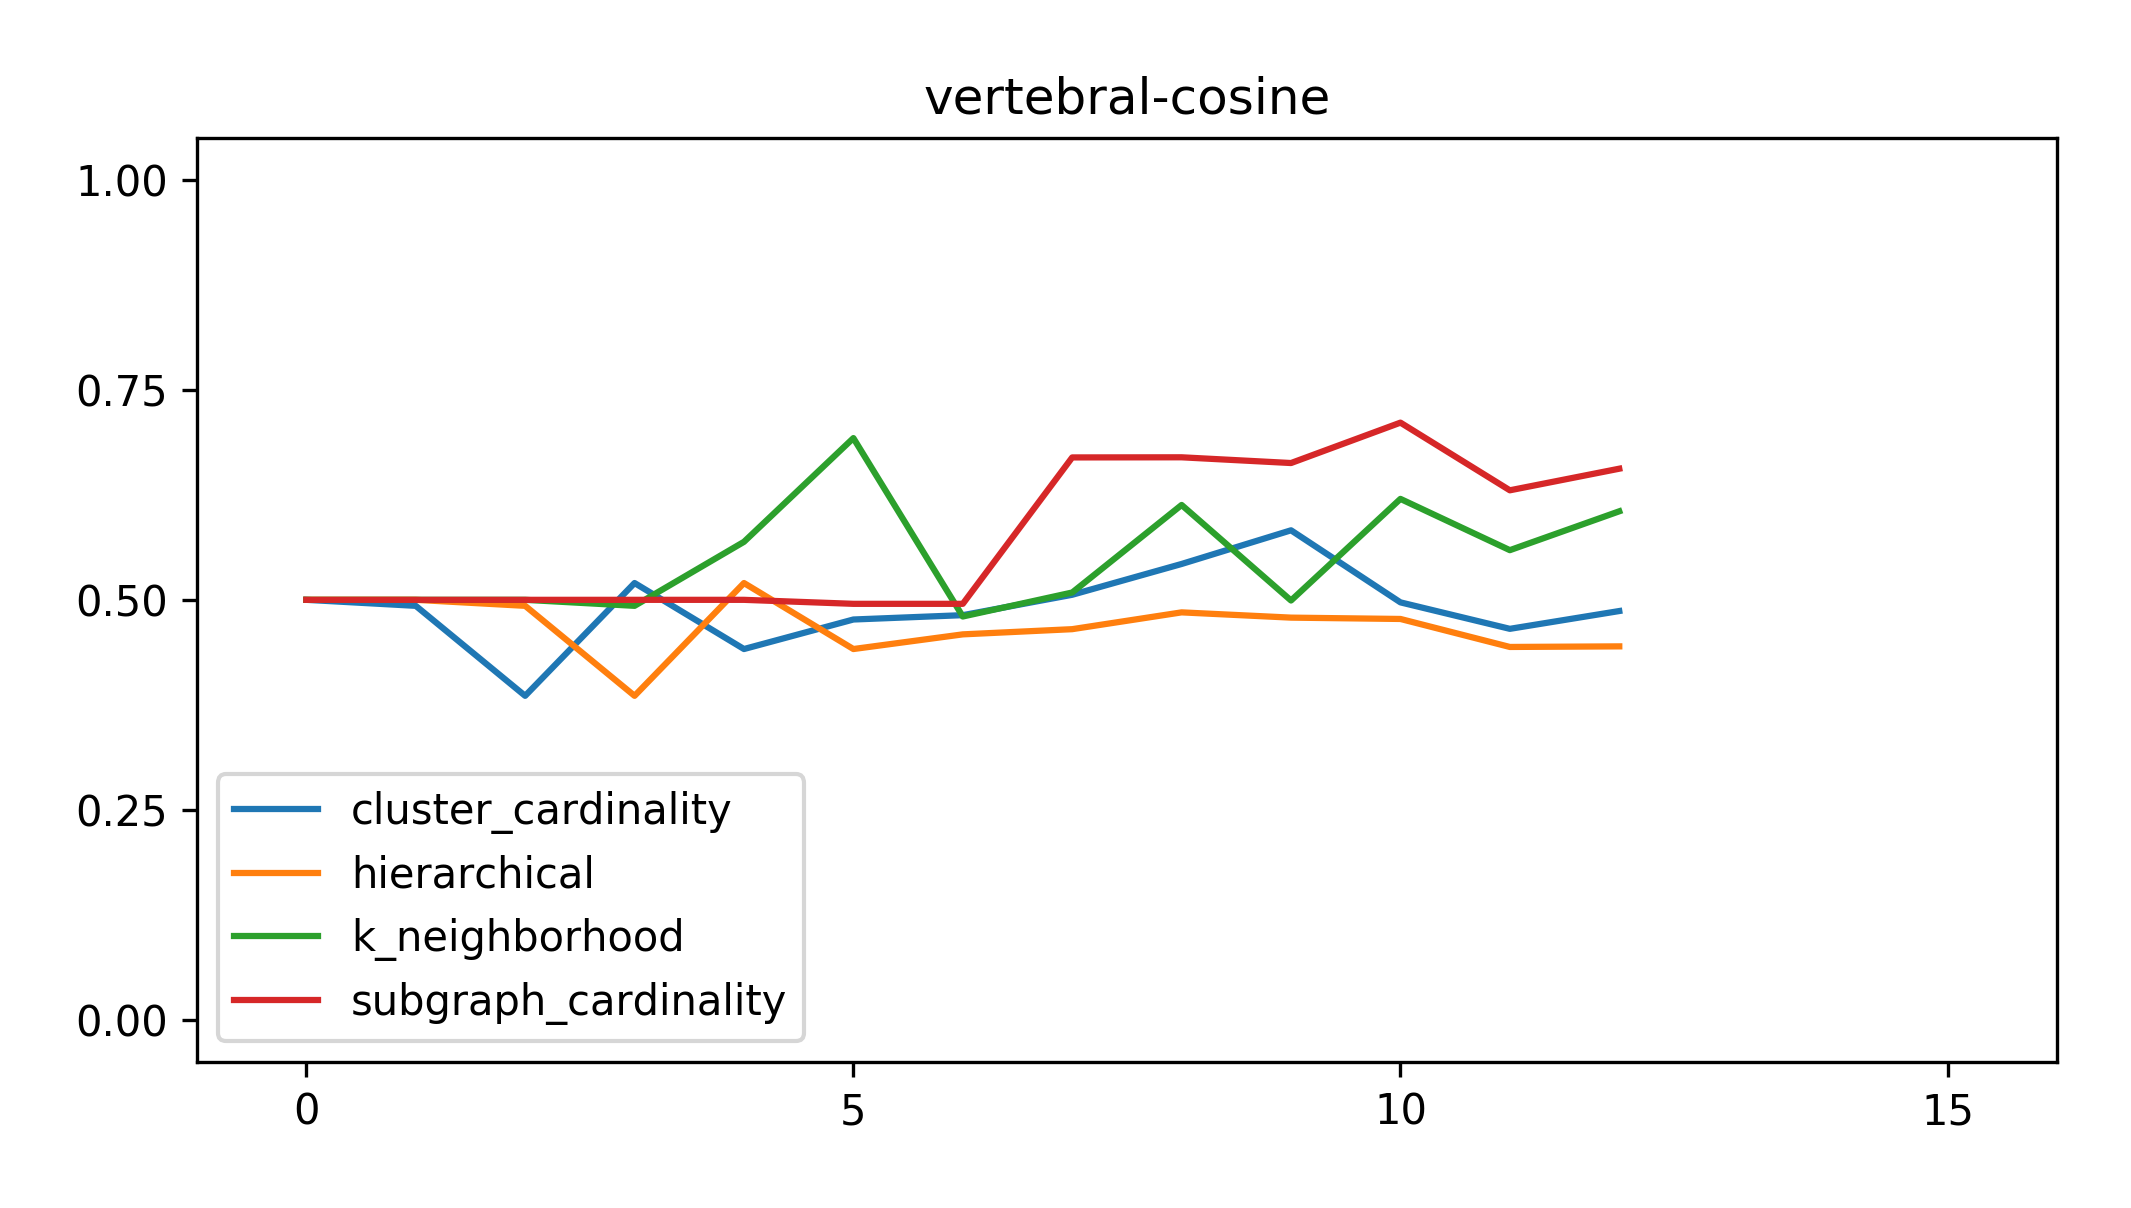
\includegraphics[width=2.2in]{kdd/static/auc_vs_depth/vertebral-cosine.png}
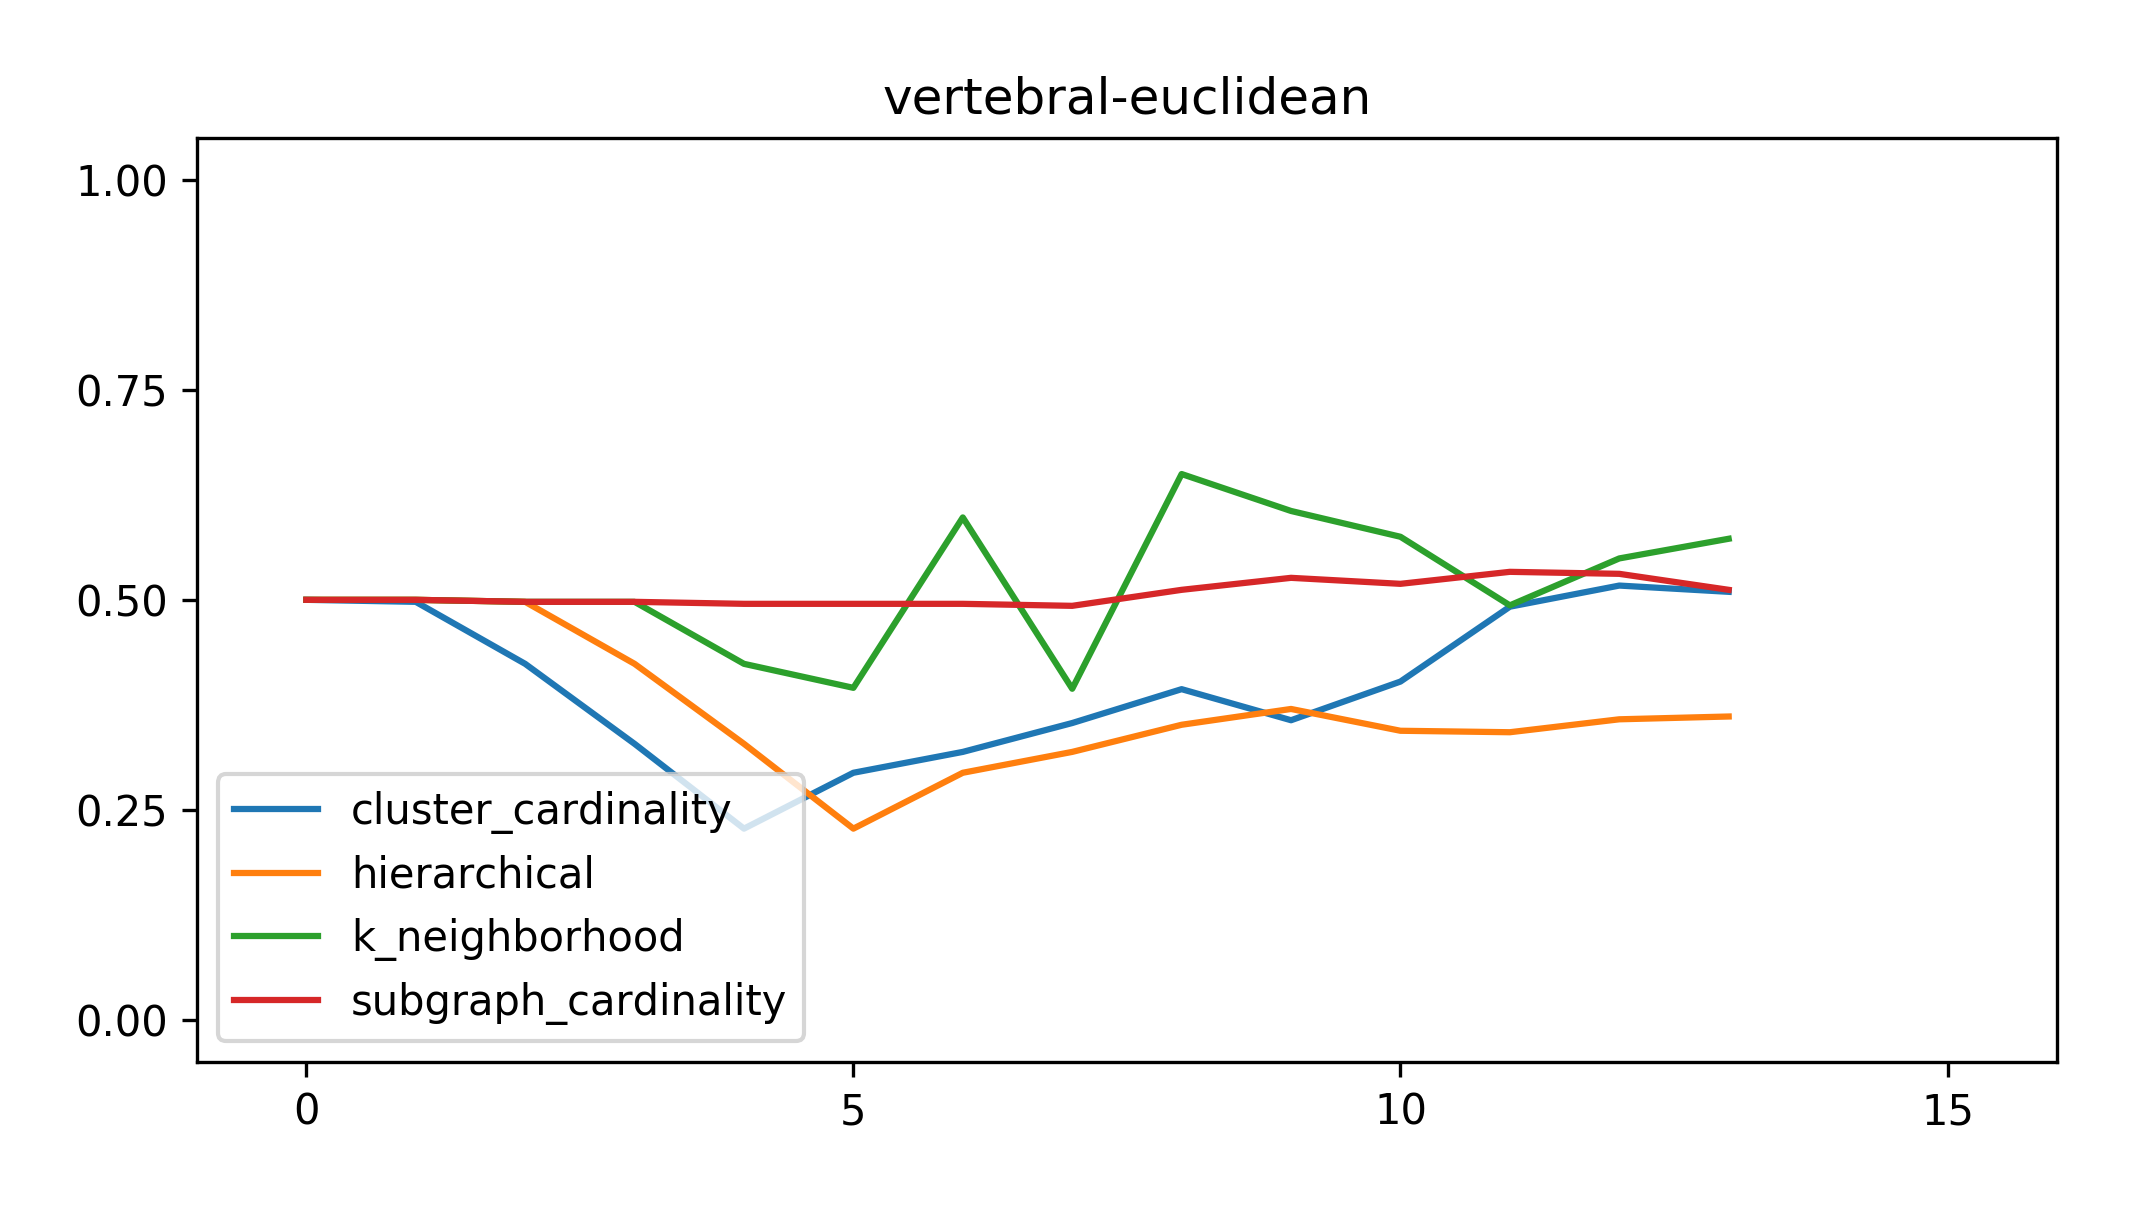
\includegraphics[width=2.2in]{kdd/static/auc_vs_depth/vertebral-euclidean.png}
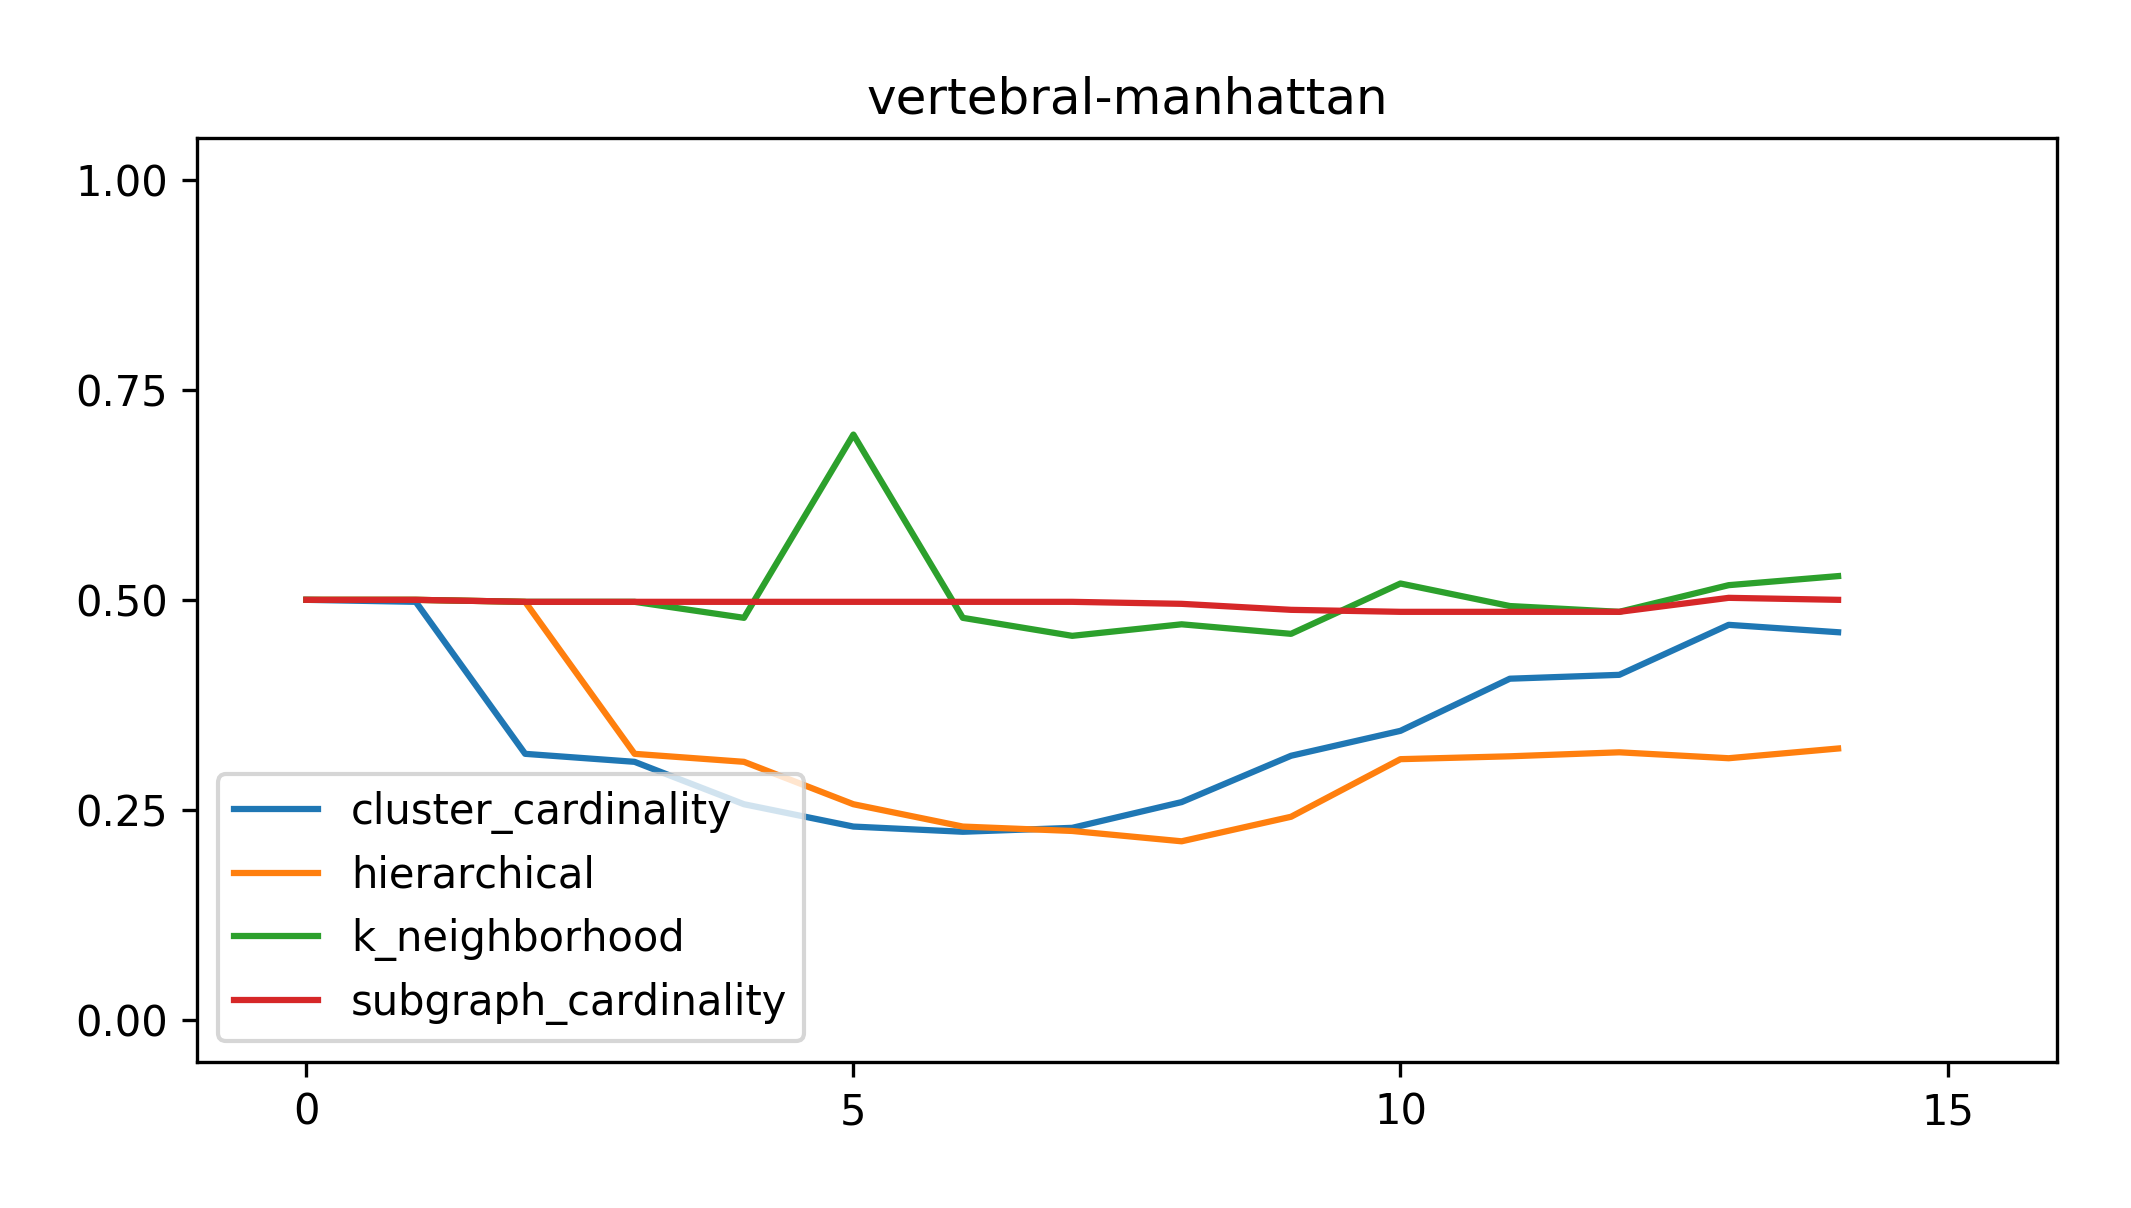
\includegraphics[width=2.2in]{kdd/static/auc_vs_depth/vertebral-manhattan.png}

% Vowels
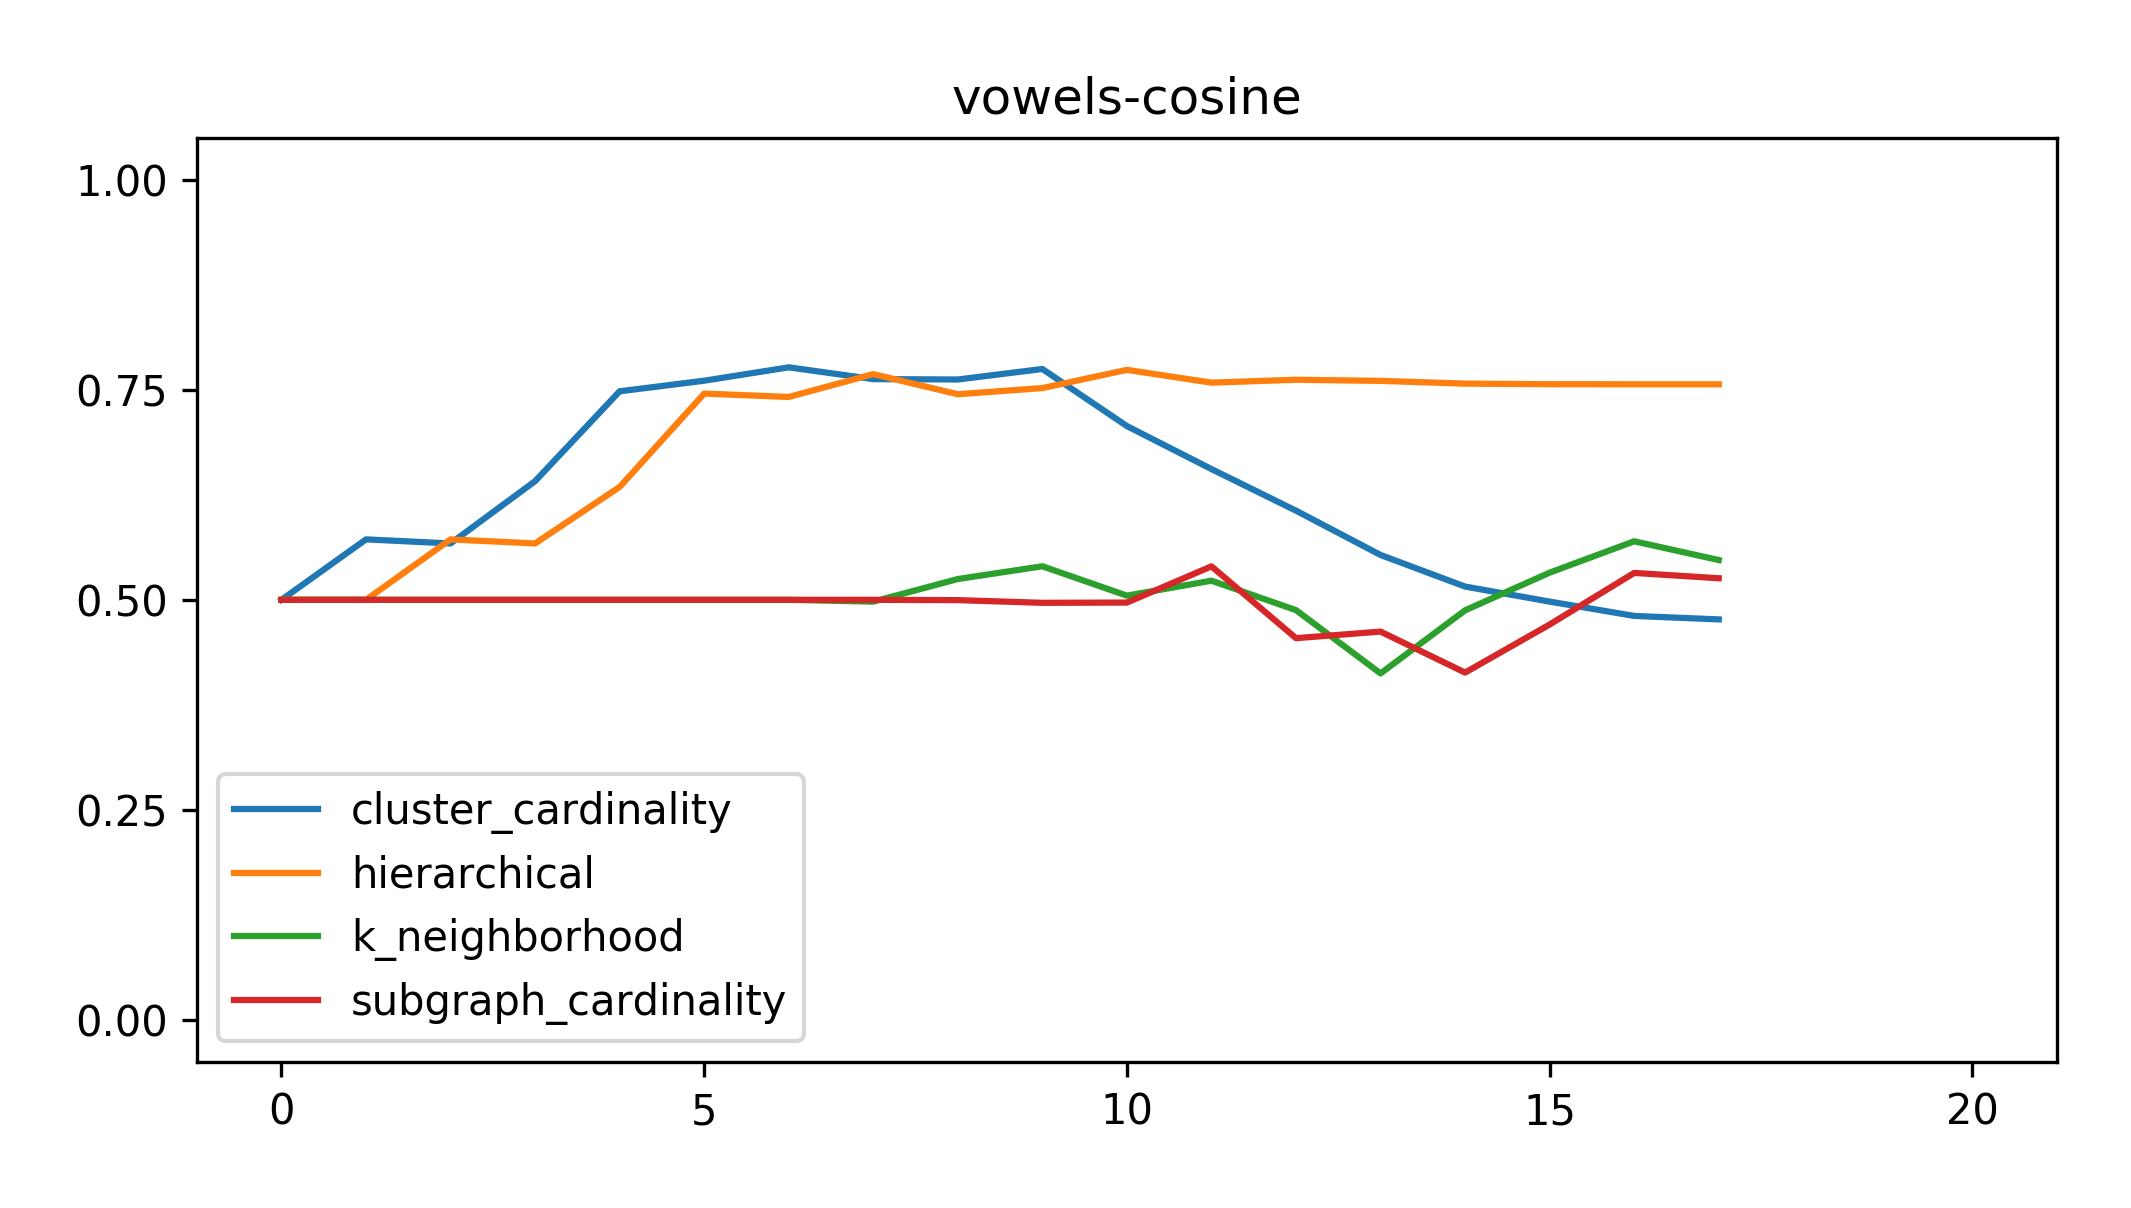
\includegraphics[width=2.2in]{kdd/static/auc_vs_depth/vowels-cosine.png}
\includegraphics[width=2.2in]{kdd/static/auc_vs_depth/vowels-euclidean.png}
\includegraphics[width=2.2in]{kdd/static/auc_vs_depth/vowels-manhattan.png}

% WBC
\includegraphics[width=2.2in]{kdd/static/auc_vs_depth/wbc-cosine.png}
\includegraphics[width=2.2in]{kdd/static/auc_vs_depth/wbc-euclidean.png}
\includegraphics[width=2.2in]{kdd/static/auc_vs_depth/wbc-manhattan.png}

% Wine
\includegraphics[width=2.2in]{kdd/static/auc_vs_depth/wine-cosine.png}
\includegraphics[width=2.2in]{kdd/static/auc_vs_depth/wine-euclidean.png}
\includegraphics[width=2.2in]{kdd/static/auc_vs_depth/wine-manhattan.png}

% HTTP
\includegraphics[width=2.2in]{kdd/static/auc_vs_depth/http-cosine.png}
\includegraphics[width=2.2in]{kdd/static/auc_vs_depth/http-euclidean.png}
\includegraphics[width=2.2in]{kdd/static/auc_vs_depth/http-manhattan.png}

\caption{
Plots of ROC-AUC vs Depth for our mearures of Anomolousness.
}

\label{results:datasets_3}
\end{figure*}

\begin{figure*}[!t]
\centering
% SMTP
\includegraphics[width=2.2in]{kdd/static/auc_vs_depth/smtp-cosine.png}
\includegraphics[width=2.2in]{kdd/static/auc_vs_depth/smtp-euclidean.png}
\includegraphics[width=2.2in]{kdd/static/auc_vs_depth/smtp-manhattan.png}

% Pendigits
\includegraphics[width=2.2in]{kdd/static/auc_vs_depth/pendigits-cosine.png}
\includegraphics[width=2.2in]{kdd/static/auc_vs_depth/pendigits-euclidean.png}
\includegraphics[width=2.2in]{kdd/static/auc_vs_depth/pendigits-manhattan.png}

% Mammography
\includegraphics[width=2.2in]{kdd/static/auc_vs_depth/mammography-cosine.png}
\includegraphics[width=2.2in]{kdd/static/auc_vs_depth/mammography-euclidean.png}
\includegraphics[width=2.2in]{kdd/static/auc_vs_depth/mammography-manhattan.png}

\caption{
Plots of ROC-AUC vs Depth for our mearures of Anomolousness.
}

\label{results:datasets_4}
\end{figure*}

